%! program = pdflatex

\documentclass[12pt]{article}

%%% PACKAGES
\usepackage{ifpdf}
\usepackage{booktabs}   % for much better looking tables
\usepackage{array}      % for better arrays (eg matrices) in maths
\usepackage{paralist}   % very flexible & customisable lists (eg. enumerate/itemize, etc.)
%\usepackage{verbatim}   % adds environment for commenting out blocks of text & for better verbatim
\usepackage{subfigure}  % make it possible to include more than one captioned figure/table in a single float
% These packages are all incorporated in the memoir class to one degree or another...
\ifpdf
\usepackage[pdftex]{graphicx}
\else
\usepackage[dvips]{graphicx}
\fi
\usepackage{epstopdf}
\usepackage[cmex10]{amsmath}
\interdisplaylinepenalty=2500

%%% PAGE DIMENSIONS
\usepackage{geometry} % to change the page dimensions
\geometry{letterpaper}
%\geometry{margins=2in} % for example, change the margins to 2 inches all round
%\geometry{landscape} % set up the page for landscape
% read geometry.pdf for detailed page layout information

%% HEADERS & FOOTERS
\usepackage{fancyhdr} % This should be set AFTER setting up the page geometry
\pagestyle{fancy} % options: empty , plain , fancy
\renewcommand{\headrulewidth}{0pt} % customise the layout...
%\lhead{}\chead{}\rhead{\hl{--- DRAFT ---}}
\lhead{}\chead{}\rhead{}
\lfoot{}\cfoot{\thepage}\rfoot{}

% *** MY ADDITIONAL PACKAGES ***
\usepackage{amsfonts}
\usepackage{amstext}
%\usepackage{ctable}        % messes up table captions among other things
\usepackage{booktabs}       % defines \toprule, \midrule, \bottomrule
\usepackage{threeparttable} % needed for table notes
%\usepackage{longtable}      % for multi-page tables
%\usepackage[font=normalsize]{caption}   % to keep caption for multi-page
                            % table normal size after using \footnotesize
                            % to reduce rest of table
%\usepackage{multirow}
%\usepackage{mathenv}
\usepackage{textcomp}      % improves \textregistered, provides \textquotesingle
\usepackage[usenames]{color}
\usepackage{soul}
\usepackage{fancyvrb}
\usepackage{relsize}
\usepackage[noadjust]{cite} % prevent adding a space
%\usepackage{url}
\usepackage{xr-hyper}
\usepackage[usenames,dvipsnames,svgnames,table]{xcolor} % additional named colors
\usepackage[colorlinks=true,urlcolor=blue,hyperfootnotes=false,backref=section,citecolor=LimeGreen]{hyperref}
%\usepackage[colorlinks=true,urlcolor=blue,hyperfootnotes=false]{hyperref}
% These are (supposedly) the defaults
% \hypersetup{
%     bookmarks=true,         % show bookmarks bar?
%     unicode=false,          % non-Latin characters in Acrobat's bookmarks
%     pdftoolbar=true,        % show Acrobat's toolbar?
%     pdfmenubar=true,        % show Acrobat's menu?
%     pdffitwindow=true,      % page fit to window when opened
%     pdftitle={My title},    % title
%     pdfauthor={Author},     % author
%     pdfsubject={Subject},   % subject of the document
%     pdfcreator={Creator},   % creator of the document
%     pdfproducer={Producer}, % producer of the document
%     pdfkeywords={keywords}, % list of keywords
%     pdfnewwindow=true,      % links in new window
%     colorlinks=false,       % false: boxed links; true: colored links
%     linkcolor=red,          % color of internal links
%     citecolor=green,        % color of links to bibliography
%     filecolor=magenta,      % color of file links
%     urlcolor=cyan           % color of external links
% }
\usepackage{upquote}        % single quotes in verbatim environments
\usepackage[title,titletoc]{appendix}

%%% SECTION TITLE APPEARANCE
% \usepackage{sectsty}
% \allsectionsfont{\sffamily\mdseries\upshape} % (See the fntguide.pdf for font help)
% (This matches ConTeXt defaults)

%%% ToC APPEARANCE
\usepackage[nottoc,notlof,notlot]{tocbibind} % Put the bibliography in the ToC
% \usepackage[titles]{tocloft} % Alter the style of the Table of Contents
% \renewcommand{\cftsecfont}{\rmfamily\mdseries\upshape}
% \renewcommand{\cftsecpagefont}{\rmfamily\mdseries\upshape} % No bold!

% Namelist environment generates a list with an item width of your choice.
% Syntax:  \begin{namelist}{widthstring} .  From Buerger's book.
\newcommand{\namelistlabel}[1]{\mbox{#1}\hfil}
\newenvironment{namelist}[1]{%
\begin{list}{}
  {
    \let\makelabel\namelistlabel
    \settowidth{\labelwidth}{#1}
    \setlength{\leftmargin}{1.1\labelwidth}
  }
 }{%
\end{list}}

% define my verbatim environment, requires packages fancyvrb & relsize
\renewcommand{\FancyVerbFormatLine}[1]{\makebox[2mm][l]{}#1}
\DefineVerbatimEnvironment%
  {Code}{Verbatim}
  {fontsize=\relsize{-1.5},
  samepage=true,
  frame=single}

% define my verbatim environment, requires packages fancyvrb & relsize
\renewcommand{\FancyVerbFormatLine}[1]{\makebox[2mm][l]{}#1}
\DefineVerbatimEnvironment%
  {Notice}{Verbatim}
  {fontsize=\relsize{-1.5},
  samepage=true,
  xleftmargin=15mm,
  framesep=5mm,
  frame=single}

%% makes verbatim text 'small' (using verbatim package)
%\makeatletter
%\g@addto@macro\@verbatim\small
%\makeatother

%\hyphenation{matpower}

\newcommand{\mpver}[0]{7.0}
%\newcommand{\matlab}[0]{{Matlab}}
%\newcommand{\matlab}[0]{{\sc Matlab}\textsuperscript{\tiny \textregistered}}
\newcommand{\matlab}[0]{{\sc Matlab}}
\newcommand{\matpower}[0]{{\sc Matpower}}
\newcommand{\matpowerurl}[0]{https://matpower.org}
\newcommand{\matpowerlink}[0]{\href{\matpowerurl}{\matpower{}}}
\newcommand{\matpowergithuburl}[0]{https://github.com/MATPOWER/matpower}
\newcommand{\mptest}[0]{{MP-Test}}
\newcommand{\mptesturl}[0]{https://github.com/MATPOWER/mptest}
\newcommand{\mptestlink}[0]{\href{\mptesturl}{\mptest{}}}
\newcommand{\mips}[0]{{MIPS}}
\newcommand{\mipsurl}[0]{https://github.com/MATPOWER/mips}
\newcommand{\mipslink}[0]{\href{\mipsurl}{\mips{}}}
\newcommand{\mipsname}[0]{{{\bf M}{\sc atpower} \textbf{I}nterior \textbf{P}oint \textbf{S}olver}}
\newcommand{\mipsver}[0]{1.3.1}
\newcommand{\most}[0]{{MOST}}
\newcommand{\mostname}[0]{{{\bf M}{\sc atpower} \textbf{O}ptimal \textbf{S}cheduling \textbf{T}ool}}
\newcommand{\mosturl}[0]{https://github.com/MATPOWER/most}
\newcommand{\mostver}[0]{1.0.3-dev}
\newcommand{\md}[0]{{\most{} Data struct}}
\newcommand{\powerweb}[0]{{\sc PowerWeb}}
\newcommand{\pserc}[0]{{\sc PSerc}}
\newcommand{\PSERC}[0]{{Power Systems Engineering Research Center (\pserc{})}}
\newcommand{\certs}[0]{{\sc Certs}}
\newcommand{\CERTS}[0]{{Consortium for Electric Reliability Technology Solutions (\certs{})}}
\newcommand{\ipopt}[0]{{\sc Ipopt}}
\newcommand{\knitro}[0]{{Artelys Knitro}}
\newcommand{\clp}[0]{{CLP}}
\newcommand{\cplex}[0]{{CPLEX}}
\newcommand{\glpk}[0]{{GLPK}}
\newcommand{\gurobi}[0]{{Gurobi}}
\newcommand{\mosek}[0]{{MOSEK}}
\newcommand{\ot}[0]{{Optimization Toolbox}}
\newcommand{\pardiso}[0]{{PARDISO}}
\newcommand{\sdppf}[0]{\texttt{SDP\_PF}}
\newcommand{\sdppfver}[0]{1.0.1}
\newcommand{\sdpopf}[0]{SDPOPF}
\newcommand{\code}[1]{{\relsize{-0.5}{\tt{{#1}}}}}  % requires package relsize
% Note: to get straight single quotes in \code you have to use one of the
%       following: \char13 \char'15 \char"0D \textquotesingle
\newcommand{\codeq}[1]{\code{\textquotesingle{}#1\textquotesingle}}  % requires package textcomp
\newcommand{\mppath}[1]{\textsf{\textsl{{\relsize{-1.0}\textless{}\mbox{MATPOWER}\textgreater{}}}}\code{{#1}}}  % requires package relsize
%\newcommand{\mostpath}[1]{\code{\$MOST{#1}}}
\newcommand{\mipspath}[1]{\textsf{\textsl{{\relsize{-1.0}\textless{}\mbox{MIPS}\textgreater{}}}}\code{{#1}}}  % requires package relsize
\newcommand{\mostpath}[1]{\mppath{}\code{/most{#1}}}
\newcommand{\mostpathb}[1]{\textsf{\textsl{{\relsize{-1.0}\textless{}\mbox{MOST}\textgreater{}}}}\code{{#1}}}  % requires package relsize
\newcommand{\baseMVA}[0]{\code{baseMVA}}
\newcommand{\bus}[0]{\code{bus}}
\newcommand{\branch}[0]{\code{branch}}
\newcommand{\gen}[0]{\code{gen}}
\newcommand{\gencost}[0]{\code{gencost}}
\newcommand{\areas}[0]{\code{areas}}
\newcommand{\mpc}[0]{\code{mpc}}
\newcommand{\results}[0]{\code{results}}
%\newcommand{\distname}[0]{\code{mostNNN}}
%\newcommand{\zipname}[0]{\code{mostNNN.zip}}
\newcommand{\mumurl}[0]{https://matpower.org/docs/MATPOWER-manual-\mpver.pdf}
\newcommand{\mum}[0]{\href{\mumurl}{\matpower{} User's Manual}}
\newcommand{\mipsmanurl}[0]{https://matpower.org/docs/MIPS-manual-\mipsver.pdf}
\newcommand{\mostmanurl}[0]{https://matpower.org/docs/MOST-manual-\mostver.pdf}
\newcommand{\currentmumurl}[0]{https://matpower.org/docs/MATPOWER-manual.pdf}
\newcommand{\currentmipsmanurl}[0]{https://matpower.org/docs/MIPS-manual.pdf}
\newcommand{\currentmostmanurl}[0]{https://matpower.org/docs/MOST-manual.pdf}
\newcommand{\mipsman}[0]{\href{\mipsmanurl}{\mips{} User's Manual}}
\newcommand{\mostman}[0]{\href{\mostmanurl}{\most{} User's Manual}}
\newcommand{\dg}[0]{\sp\dagger}                         % hermitian conjugate
%\newcommand{\trans}[1]{{#1}^{\ensuremath{\mathsf{T}}}}  % transpose
\newcommand{\trans}[1]{#1^{\ensuremath{\mathsf{T}}}}    % transpose
\newcommand{\cc}[1]{{#1}^{\ast}}                        % complex conjugate
\newcommand{\hc}[1]{{#1}^{\dg}}                         % hermitian conjugate
\newcommand{\conj}[1]{{#1}^{+}}                         % hermitian conjugate
\newcommand{\diag}[1]{\left[{#1}\right]}                % diagonal
\newcommand{\R}{\mathbb{R}}          % requires \usepackage{amsfonts|bbold}
\newcommand{\der}[2]{\frac{\partial{#1}}{\partial{#2}}} % partial derivative
\newcommand{\doi}[1]{doi:~\href{https://doi.org/#1}{#1}}

\def\sectionautorefname{Chapter}
\def\subsectionautorefname{Section}
\def\subsubsectionautorefname{Section}
\newcommand{\secref}[1]{\autoref{#1} \nameref{#1}}

\numberwithin{equation}{section}
\numberwithin{table}{section}
\renewcommand{\thetable}{\thesection\mbox{-}\arabic{table}}
\numberwithin{figure}{section}
\renewcommand{\thefigure}{\thesection\mbox{-}\arabic{figure}}

\externaldocument[MUM-]{MATPOWER-manual}[\mumurl]

%\title{\hl{--- DRAFT  ---}\\\hl{\em do not distribute}\\~\\\mostname{}\\\most{} \mostver{}\\
\title{\mostname{}\\\most{} \mostver{}\\
User's Manual}
\author{Ray~D.~Zimmerman \and Carlos~E.~Murillo-S\'anchez}
%%% BEFORE PUBLISHING A NEW VERSION:
%%%   Update the publication year for \bibitem{matpower} and
%%%   \bibitem{matpower_manual} to the year of the latest release
%\date{June 20, 2019} % comment this line to display the current date
%\date{December 14, 2011\thanks{Second revision. First revision was December 13, 2011}} % comment this line to display the current date

%%% BEGIN DOCUMENT
\begin{document}
\maketitle
\thispagestyle{empty}
\vfill
\begin{center}
{\scriptsize
\copyright~2011--2019~\PSERC{}\\
All Rights Reserved}
\end{center}

\clearpage
%\setcounter{page}{2}
\tableofcontents
\clearpage
\listoffigures
\listoftables

%%------------------------------------------
\clearpage
\section{Introduction}

Beginning with version 6, \matpower{}~\cite{zimmerman2011,matpower,matpower_manual} includes a framework for solving generalized steady-state electric power scheduling problems. This framework is known as \most{}, for \mostname{}~\cite{murillo-sanchez2013a,lamadrid2018}.

\most{} can be used to solve problems as simple as a deterministic, single period economic dispatch problem with no transmission constraints or as complex as a stochastic, security-constrained, combined unit-commitment and multiperiod optimal power flow problem with locational contingency and load-following reserves, ramping costs and constraints, deferrable demands, lossy storage resources and uncertain renewable generation.

While the problem formulation is general and incorporates a full nonlinear AC network model, the current implementation is limited to DC power flow modeling of the network. Some work has been done on an AC implementation, but it is not yet ready for release.

The primary developers of \most{} are Carlos~E.~Murillo-S\'anchez\footnote{Universidad Nacional de Colombia, Manizales, Colombia} and Ray~D.~Zimmerman\footnote{Cornell University, Ithaca, NY, USA} of \pserc{}\footnote{\url{http://pserc.org/}}, with significant contributions from Daniel Mu\~noz-\'Alvarez and Alberto~J.~Lamadrid. It is built on top of \matpowerlink{}\footnote{See \url{\matpowerurl} for more information on \matpowerlink{}.}, a package of \matlab{}\textsuperscript{\tiny \textregistered} M-files for solving power flow and optimal power flow problems~\cite{zimmerman2011, zimmerman2009}. This manual assumes that the user is familiar with using \matpowerlink{}, especially for solving optimal power flow problems, and makes numerious references to version \mpver{} of the \mum{}~\cite{matpower_manual}.

%\clearpage
\subsection{License and Terms of Use}

The code in \most{} is distributed along with \matpower{} under the 3-clause BSD license~\cite{bsd}. The full text of the license can be found in the \code{LICENSE} file at the top level of the distribution or at \url{https://matpower.org/license/} and reads as follows.

\begin{Notice}
Copyright (c) 1996-2016, Power Systems Engineering Research Center
(PSERC) and individual contributors (see AUTHORS file for details).
All rights reserved.

Redistribution and use in source and binary forms, with or without
modification, are permitted provided that the following conditions
are met:

1. Redistributions of source code must retain the above copyright
notice, this list of conditions and the following disclaimer.

2. Redistributions in binary form must reproduce the above copyright
notice, this list of conditions and the following disclaimer in the
documentation and/or other materials provided with the distribution.

3. Neither the name of the copyright holder nor the names of its
contributors may be used to endorse or promote products derived from
this software without specific prior written permission.

THIS SOFTWARE IS PROVIDED BY THE COPYRIGHT HOLDERS AND CONTRIBUTORS
"AS IS" AND ANY EXPRESS OR IMPLIED WARRANTIES, INCLUDING, BUT NOT
LIMITED TO, THE IMPLIED WARRANTIES OF MERCHANTABILITY AND FITNESS
FOR A PARTICULAR PURPOSE ARE DISCLAIMED. IN NO EVENT SHALL THE
COPYRIGHT HOLDER OR CONTRIBUTORS BE LIABLE FOR ANY DIRECT, INDIRECT,
INCIDENTAL, SPECIAL, EXEMPLARY, OR CONSEQUENTIAL DAMAGES (INCLUDING,
BUT NOT LIMITED TO, PROCUREMENT OF SUBSTITUTE GOODS OR SERVICES;
LOSS OF USE, DATA, OR PROFITS; OR BUSINESS INTERRUPTION) HOWEVER
CAUSED AND ON ANY THEORY OF LIABILITY, WHETHER IN CONTRACT, STRICT
LIABILITY, OR TORT (INCLUDING NEGLIGENCE OR OTHERWISE) ARISING IN
ANY WAY OUT OF THE USE OF THIS SOFTWARE, EVEN IF ADVISED OF THE
POSSIBILITY OF SUCH DAMAGE.
\end{Notice}

\subsection{Citing \most{}}

We request that publications derived from the use of the \mostname{} (\most{}) explicitly acknowledge that fact by citing both the 2011 MATPOWER paper~\cite{zimmerman2011} and the 2013 MOST paper~\cite{murillo-sanchez2013a}.

\begin{quote}
\footnotesize
R.~D. Zimmerman, C.~E. Murillo-S{\'a}nchez, and R.~J. Thomas, ``\matpower{}: Steady-State Operations, Planning and Analysis Tools for Power Systems Research and Education,'' \emph{Power Systems, IEEE Transactions on}, vol.~26, no.~1, pp.~12--19, Feb.~2011.\\
\doi{10.1109/TPWRS.2010.2051168}
\end{quote}

\begin{quote}
\footnotesize
C.~E. Murillo-S{\'a}nchez, R.~D. Zimmerman, C.~L. Anderson, and R.~J. Thomas, ``Secure Planning and Operations of Systems with Stochastic Sources, Energy Storage and Active Demand,'' \emph{Smart Grid, IEEE Transactions on}, vol.~4, no.~4, pp.~2220--2229, Dec.~2013.\\
\doi{10.1109/TSG.2013.2281001}
\end{quote}

The \mostname{} (\most) User's Manual~\cite{most_manual} should also be
cited explicitly in work that refers to or is derived from its content.
The citation and DOI can be version-specific or general, as appropriate.
For version 1.0.2, use:

\begin{quote}
\footnotesize
R.~D. Zimmerman, C.~E. Murillo-S{\'a}nchez. \mostname{} (\most{}) User's Manual, Verision 1.0.2. 2019. [Online]. Available: \url{https://matpower.org/docs/MOST-manual-1.0.2.pdf}\\
\doi{10.5281/zenodo.3251047}
\end{quote}
For a version non-specific citation, use the following citation and DOI,
with \emph{\textless{}YEAR\textgreater{}} replaced by the year of the most recent release:

\begin{quote}
\footnotesize
R.~D. Zimmerman, C.~E. Murillo-S{\'a}nchez. \mostname{} (\most{}) User's Manual. \emph{\textless{}YEAR\textgreater{}}.
[Online]. Available: \url{https://matpower.org/docs/MOST-manual.pdf}\\
\doi{10.5281/zenodo.3236531}
\end{quote}
A list of versions of the User's Manual with release dates and
version-specific DOI's can be found via the general DOI at
\url{https://doi.org/10.5281/zenodo.3236531}.


\subsection{\most{} Development}
\label{sec:development}

Following the release of \most{} 1.0 (with \matpower{} 6.0), the \most{} project moved to an open development paradigm, hosted on the \most{} GitHub project page:

\bigskip

~~~~~~~~\url{\mosturl}

\bigskip

The \most{} GitHub project hosts the public Git code repository as well as a public issue tracker for handling bug reports, patches, and other issues and contributions. There are separate GitHub hosted repositories and issue trackers for \matpower{}, \most{}, \mips{} and the testing framework used by all of them, \mptest{}, all available from \url{https://github.com/MATPOWER/}.


%%------------------------------------------
\clearpage
\section{Getting Started}

The first step in beginning to use the \most{} is to get familiar with \matpowerlink{}. This step is essential and this manual will assume familiarity with \matpower{}.

\subsection{System Requirements}
\label{sec:sysreq}
To use \most{}~\mostver{} you will need:
\begin{itemize}
\item \matpower{} version \hl{7.1} or later\footnote{\most{}~1.0.1 required \matpower{}~7 and \most{}~1.0 required \matpower{}~6.}
\item \emph{(highly recommended)} a high-performance LP/MILP, QP/MIQP solver such as \gurobi{}, \cplex{}, \mosek{}, \matlab{}'s \ot{} or \glpk{} \emph{(included with Octave)}.
\end{itemize}

\most{} requires a working installation of \matpower{}. See the corresponding section in the \mum{} for more information on the system requirements for \matpower{}.
\matpower{}~6 and later includes a full version of \most{} in the \mostpath{} directory.

It is also highly recommended that you install a high-performance solver such as \gurobi{}, \cplex{}, \mosek{}, \matlab{}'s \ot{} or \glpk{}, described in Appendix~\ref{MUM-app:optional_packages} in the \mum{}.
For problems involving unit-commitment, a mixed integer solver is required.\footnote{At the time of this writing, \matlab{}'s \ot{} and \glpk{} only address MILP problems. \gurobi{}, \cplex{} and \mosek{} all handle MIQP problems as well.}
But even for continuous LP and QP problems, these solvers will offer much better performance than \matpower{}'s built-in solver based on \code{qps\_mips}. The problems \most{} generates can quickly become \emph{very} large, so using the best solver you have available is a priority.\footnote{\gurobi{} and \cplex{} are currently our preferred solvers for most \most{} problems.}

\subsection{Installation}

The preferred method of installation is simply to install \matpower{}, which
is a prerequisite for \most{} and also includes its own copy of \most{}.

If you have followed the directions for installing \matpower{} found in Section~\ref{MUM-sec:installation} of the \mum{}, then \most{} should already be installed in the \mostpath{} directory and the appropriate paths\footnote{To use \most{} your \matlab{} path must include \mostpath{/lib} and, to run the tests, \mostpath{/lib/t}.} added to your \matlab{} path.

To run the test suite and verify that \most{} is properly installed and functioning, at the \matlab{} prompt, type \code{test\_most} . The result should resemble the following, possibly including extra tests, depending on the availablility of optional packages.
% UPDATE BEFORE RELEASE
\begin{Code}
>> test_most
>> test_most
t_most_3b_1_1_0........ok
t_most_3b_3_1_0........ok
t_most_30b_1_1_0.......ok
t_most_30b_3_1_0.......ok
t_most_fixed_res.......ok
t_most_30b_1_1_0_uc....ok
t_most_uc..............ok
t_most_suc.............ok
t_most_w_ds............ok
All tests successful (615 of 615)
Elapsed time 84.68 seconds.
\end{Code}

If, for some reason, you prefer to install your own copy of MOST directly
from the \most{} GitHub repository\footnote{\url{https://github.com/MATPOWER/most}},
simply clone the repository to the
location of your choice, where we use \mostpathb{} to denote the path the
resulting \code{most} directory. Then add the following directories to your \matlab{} or Octave path:
\begin{itemize}
\setlength{\itemsep}{0pt}
\setlength{\parskip}{0pt}
\item \mostpathb{/lib} -- core \most{} functions
\item \mostpathb{/lib/t} -- test scripts for \most{}
\end{itemize}
It is important that they appear before \matpower{} in your path if you want
to use this version of \most{}, rather than the one included with \matpower{}.

\subsection{Running a Simulation}

Running a \most{} simulation involves (1)~preparing the input data defining all of the relevant power system parameters, transition probabilities, additional generator data and offers, storage data, contingencies, and profiles (2)~invoking the function to run the simulation and (3)~accessing the results in the output data structures. The input data is provided in a \md{} and the results are returned in an updated version of the input data structure.

Since \most{} is built upon \matpower{}, it is assumed that the user is already familiar with running OPF simulations in \matpower{} (see Section~\ref{MUM-sec:runsimulation} in the \mum{}).


\subsubsection{Preparing Input Data}

The \md{}, containing all of the data needed for the problem, is sufficiently complex that it is not typically created directly, but rather is assembled from numerous other files or data structures by the \code{loadmd} function, as described in Section~\ref{sec:inputdata}.
They consist of (1)~a \matpower{} case file or struct describing the system parameters for the base case, (2)~transition probability matrices, (3)~additional generator parameters, including commitment parameters, offer parameters related to reserves, inc/dec prices, and bounds on energy contract amounts, (4)~parameters for storage units, (5)~a contingency table defining a credible set of contingencies and their probabilities, and (6)~profiles for time varying parameters such as load and renewable availability.
In addition to the input data, aspects of the simulation are controlled by a set of \matpower{} options.

Typically, the \matpower{} case is defined in a case file and loaded into a struct using the \code{loadcase} function.
The transition probability matrices can be specified as desired via a user-defined script or function as shown in the example below.
The additional generator parameters are typically provided in a file defining an \code{xGenDataTable} and loaded by the \code{loadxgendata} function.
Both the \matpower{} case and the \code{xGenData} can be modified by adding wind generators, or generators that represent energy storage units, using the functions \code{addwind} and \code{addstorage}, respectively.
The latter also loads the additional storage parameters into a \code{StorageData} struct.
The contingency table can be provided directly or returned by a user-defined function and is a changes table (\code{chgtab}) in the form expected by \matpower{}'s \code{apply\_changes} function.\footnote{See Section~\ref{MUM-sec:apply_changes} in the \mum{}.}
And any time-varying parameters, such as load scaling factors and wind availability, are specified in profile data files and loaded with the \code{getprofiles} function.

% Finally, the pieces are all assembled into a \md{} by the \code{loadmd} function.
% See Section~\ref{sec:inputdata} for details on each input argument.

\begin{Code}
mpc = loadcase('ex_case3b');
transmat = ex_transmat(12);
xgd = loadxgendata('ex_xgd_uc', mpc);
[iwind, mpc, xgd] = addwind('ex_wind_uc', mpc, xgd);
[iess, mpc, xgd, sd] = addstorage('ex_storage', mpc, xgd);
contab = ex_contab();
profiles = getprofiles('ex_load_profile');
profiles = getprofiles('ex_wind_profile', profiles, iwind);
mdi = loadmd(mpc, transmat, xgd, sd, contab, profiles);
mpopt = mpoption('verbose', 0);
\end{Code}

\subsubsection{Solving the Case}

The solver in \most{} is implemented in the \code{most} function. Assuming the input data have been loaded into the input \md{} (\code{mdi}) and the \matpower{} options set in \code{mpopt}, the first stage solver can be called as follows.
\begin{Code}
mdo = most(mdi, mpopt);
\end{Code}

\begin{Code}
=============================================================================
          MATPOWER Optimal Scheduling Tool  --  MOST Version 1.0.2
          A multiperiod stochastic secure OPF with unit commitment
                       -----  Built on MATPOWER  -----
  by Carlos E. Murillo-Sanchez, Universidad Nacional de Colombia--Manizales
                  and Ray D. Zimmerman, Cornell University
       (c) 2012-2019 Power Systems Engineering Research Center (PSERC)       
=============================================================================
- Building indexing structures.
- Building expected storage-tracking mechanism.
- Building constraint submatrices.
  - Building DC flow constraints.
  - Splitting storage injections into charge/discharge.
  - Building CCV constraints for piecewise-linear costs.
  - Building contingency reserve constraints.
  - Building ramping transitions and reserve constraints.
  - Building storage constraints.
  - Building unit commitment constraints.
- Building cost structures.
- Assembling full set of costs.
- Assembling full set of constraints.
- Assembling full set of variable bounds.
- Calling MILP solver.

============================================================================

Gurobi Version 8.1.1 -- automatic MILP solver
--- Integer stage complete, starting price computation stage ---
Gurobi Version 8.1.1 -- automatic LP solver

============================================================================
- MOST: MILP solved successfully.
- Post-processing results.
- MOST: Done.
\end{Code}

\subsubsection{Accessing the Results}

By default, the simulation does not output any results to the screen, instead storing the results in the output \md{} (\code{mdo}).
The details of the results in \code{mdo} can be found in Section~\ref{sec:mdoutputdata}.

For example, quantities like the commitment, expected dispatch and expected energy price, upward contingency and ramping reserve amounts for generator~$i$ in period~$t$, and the dispatch of generator~$i$ in period~$t$, scenario~$j$ and contingency~$k$ can be extracted as follows.
\begin{Code}
define_constants;
unit_commitment     = mdo.UC.CommitSched(i, t);
expected_dispatch   = mdo.results.ExpectedDispatch(i, t);
expected_price      = mdo.results.GenPrices(i, t);
cont_reserve_up     = mdo.results.Rpp(i, t);
ramp_reserve_up     = mdo.results.Rrp(i, t);
Pg_tijk             = mdo.flow(t,j,k).mpc.gen(i, PG);
\end{Code}

There is also a function called \code{most\_summary}, described in Section~\ref{sec:most_summary}, that can be used to print some summary results.

\subsubsection{Setting Options}

The standard \matpower{} options struct is used to set options such as the amount of progress output to display and algorithm to use to solve the underlying optimization problem. The options struct is set using the \code{mpoption} function.

\begin{Code}
mpopt = mpoption('verbose', 2, 'most.solver', 'GUROBI');
\end{Code}

The full set of \most{} options are detailed in Section~\ref{sec:mostoptions}.

\subsection{Documentation}

There are two primary sources of documentation for \most{}. The first is \href{\mostmanurl}{this manual}, which gives an overview of the capabilities and structure and describes the problem formulation. The \mostman{} can be found in your \matpower{} distribution at \mppath{/most/docs/MOST-manual.pdf} and the \href{\currentmostmanurl}{latest version} is always available at: \url{\currentmostmanurl}.

The second is the built-in \code{help} command. As with \matlab{}'s built-in functions and toolbox routines, you can type \code{help} followed by the name of a command or M-file to get help on that particular function. Many of the \most{} related M-files have such documentation and this should be considered the main reference for the calling options for each individual function. See Appendix~\ref{app:functions} for a list of \most{} functions.

There is one other important source of related documentation and that is the \mum{}. It is assumed that the user is very familiar with \matpower{} and its OPF capabilities.


%%------------------------------------------
\clearpage
\section{Background and Overview}

\most{} grew out of research at Cornell University on the development and testing of new tools for the power industry, funded by the U.S. Department of Energy through the CERTS Reliability and Markets program.\footnote{This work was supported by the Consortium for Electric Reliability Technology Solutions and the Office of Electricity Delivery and Energy Reliability, Transmission Reliability Program of the U.S. Department of Energy under the National Energy Technology Laboratory Cooperative Agreement No. DE-FC26-09NT43321. \url{https://certs.lbl.gov/research-areas/reliability-markets-rm}} Initially the work was focused on extending the AC optimal power flow problem to include co-optimization of locational reserves for security defined in terms of explicitly included contingencies \cite{superopf2008,murillo-sanchez2013}. This work was then extended to include multiple base scenarios to represent stochastic load and renewable generation availability, a multiperiod planning horizon, energy storage resources, ramping considerations and binary unit commitment decisions \cite{murillo-sanchez2013a}.

The formulation implemented in \most{} and described in the next section further generalizes the problem by including the facility to define zonal reserve requirements like those from Section~\ref{MUM-sec:reserves} in the \mum{}~\cite{matpower_manual}, and to constrain the solutions via a general linear time-varying dynamical system. The initial prototype was implemented by Carlos~E.~Murillo-S\'anchez with subsequent development by Ray~D.~Zimmerman along with contributions by Daniel Mu\~noz-\'Alvarez and Alberto~J.~Lamadrid.

The description of the problem formulation will begin with a conceptual overview of the approach, beginning with the simplest single period problem that \most{} handles and extending and expanding the problem one step at a time to illustrate how each additional aspect of the full problem is handled.

\subsection{Continuous Single Period Problems}

A single period problem can be as simple as a lossless economic dispatch (ED) problem, where the objective is to find the set of generator dispatch points that minimize the total cost of meeting a specified demand, with no modeling of any network flows at all. Even at this level, dispatchable demands can be introduced, modeled as negative generation as in Section~\ref{MUM-sec:dispatchable_loads} in the \mum{}, to model either involuntary load shedding or demand-side resources dispatched according to a benefit or bid function. It is assumed throughout that power injection variables may represent either generators or loads.

By introducing DC power flow equations as a function of bus voltage angle variables, along with limits on the branch flows, the problem becomes a DC OPF, taking into account transmission system limitations. Using instead the AC power flow equations and flow constraints and introducing voltage magnitude and reactive injection variables results in an AC OPF problem, which models losses along with voltage and reactive power requirements.

Figure~\ref{fig:most_single_period} illustrates the range of continuous single period problems considered by the formulation, with the varying level of detail of the network modeling represented by the vertical dimension. The horizontal dimension represents different ways to handle (or not) operational security requirements, with a third dimension adding a stochastic option for handling the uncertainty of demand and renewable generation. The green portion denotes the parts of the formulation that are implemented in the current version of \most{}.

\begin{figure}[hbtp]
  \centering
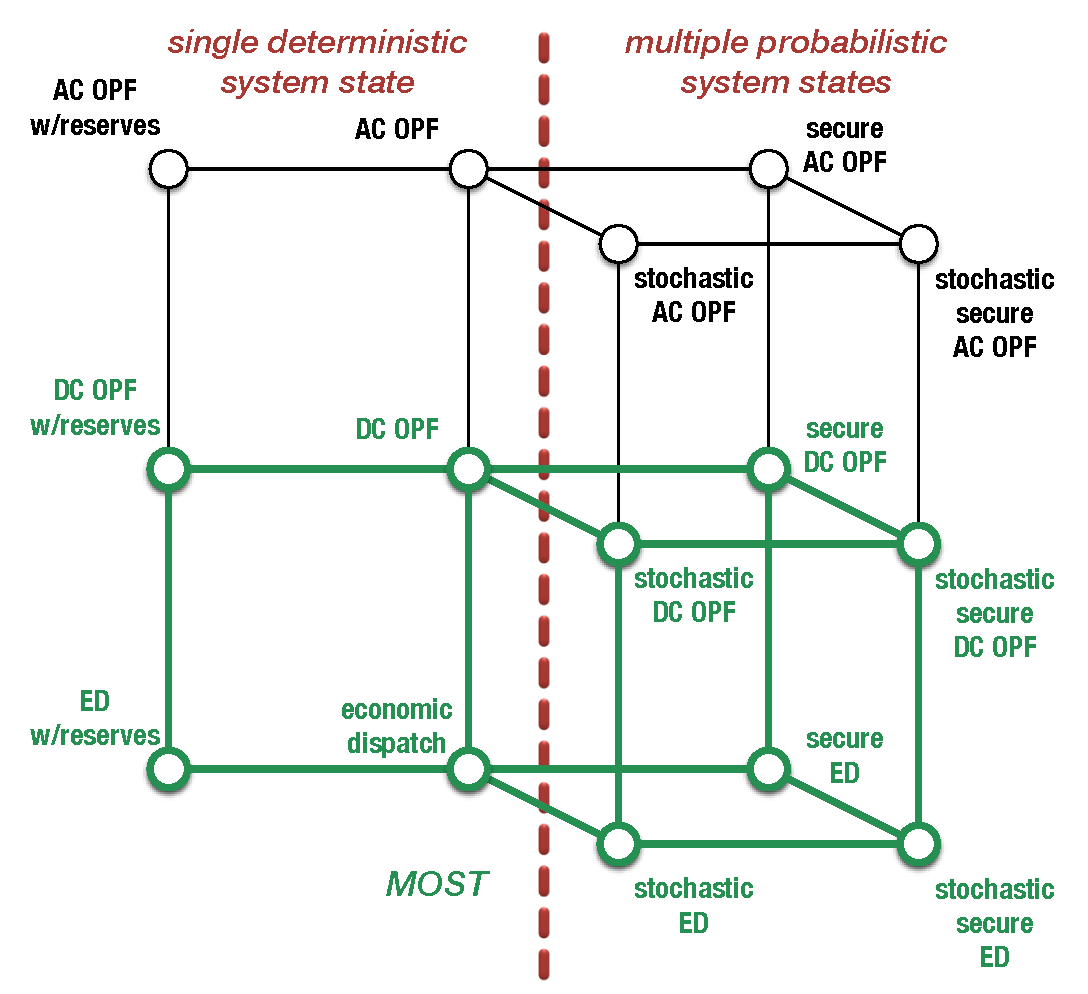
\includegraphics[width=0.8\textwidth]{./figures/most-single-period-problems-16}
  \caption{MOST Continuous Single-Period Problems}
  \label{fig:most_single_period}
\end{figure}

\subsection{Security}

Two options are included for addressing security in the single period problem, that is the need to find a dispatch that meets some criteria for withstanding disturbances or outages. The first is a deterministic approach that simply adds fixed zonal reserve requirements using the additional variables, constraints and costs described in Section~\ref{MUM-sec:reserves} in the \mum{}.

The second is a stochastic approach, based on explicitly modeling the post-contingency state for each of a set of credible contingencies. In this approach, the base case ED or OPF problem is fully duplicated (all variables, costs and constraints) for each of the contingency states and modified to reflect the outaged equipment.

The base and contingency states are then combined into one large problem, where they are treated as separate islands in a single network, with the cost of each state weighted by its probability of occurence. The base and contingency states are further tied together by ramp limits on the generators, ensuring that the contingency state dispatches can be reached from the base case while respecting ramp rate constraints.

Finally, associated with each generator is a variable representing a reference dispatch value (e.g. optimal contract value) from which dispatch deviations (incremental and decremental redispatches) are defined. The maximum upward and downward deviations from this reference dispatch across all (base and contingency) states are defined as the upward and downward contingency reserves, respectively, and these reserves can have costs associated with them. In addition, the state specific deviations from the reference quantity can have their own probability weighted redispatch costs.

This second approach to security yields security constrained dispatch (ED or OPF) problem with endogenously determined generator-specific locational reserve requirements, derived optimally as a function of the set of included credible contingencies. In this problem formulation, it is assumed that the decisions regarding a reference dispatch and the corresponding dispatch ranges that define the reserves are made before the uncertain outcome of the occurence or non-occurence of a contingency is revealed. The state specific dispatch decisions are recourse decisions contingent on the outcome of that uncertainty.

\begin{figure}[hbtp]
  \centering
  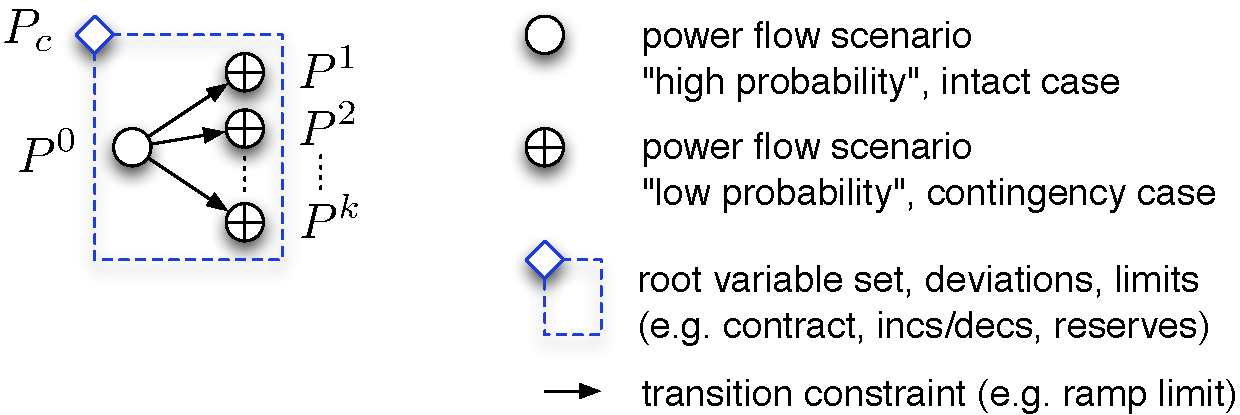
\includegraphics[width=0.8\textwidth]{./figures/structure}
  \caption{Secure Dispatch Problem Structure}
  \label{fig:secure_dispatch_structure}
\end{figure}

The structure of this problem is illustrated by the diagram in Figure~\ref{fig:secure_dispatch_structure}, where the circles represent the ED or OPF problems corresponding to the individual states, the dashed box denotes the reference dispatch, redispatches, reserves and associated costs and constraints, and the arrows illustrate the ramp limits constraining the deviations of contingency state dispatches from the base case dispatch.

\begin{figure}[hbtp]
  \centering
  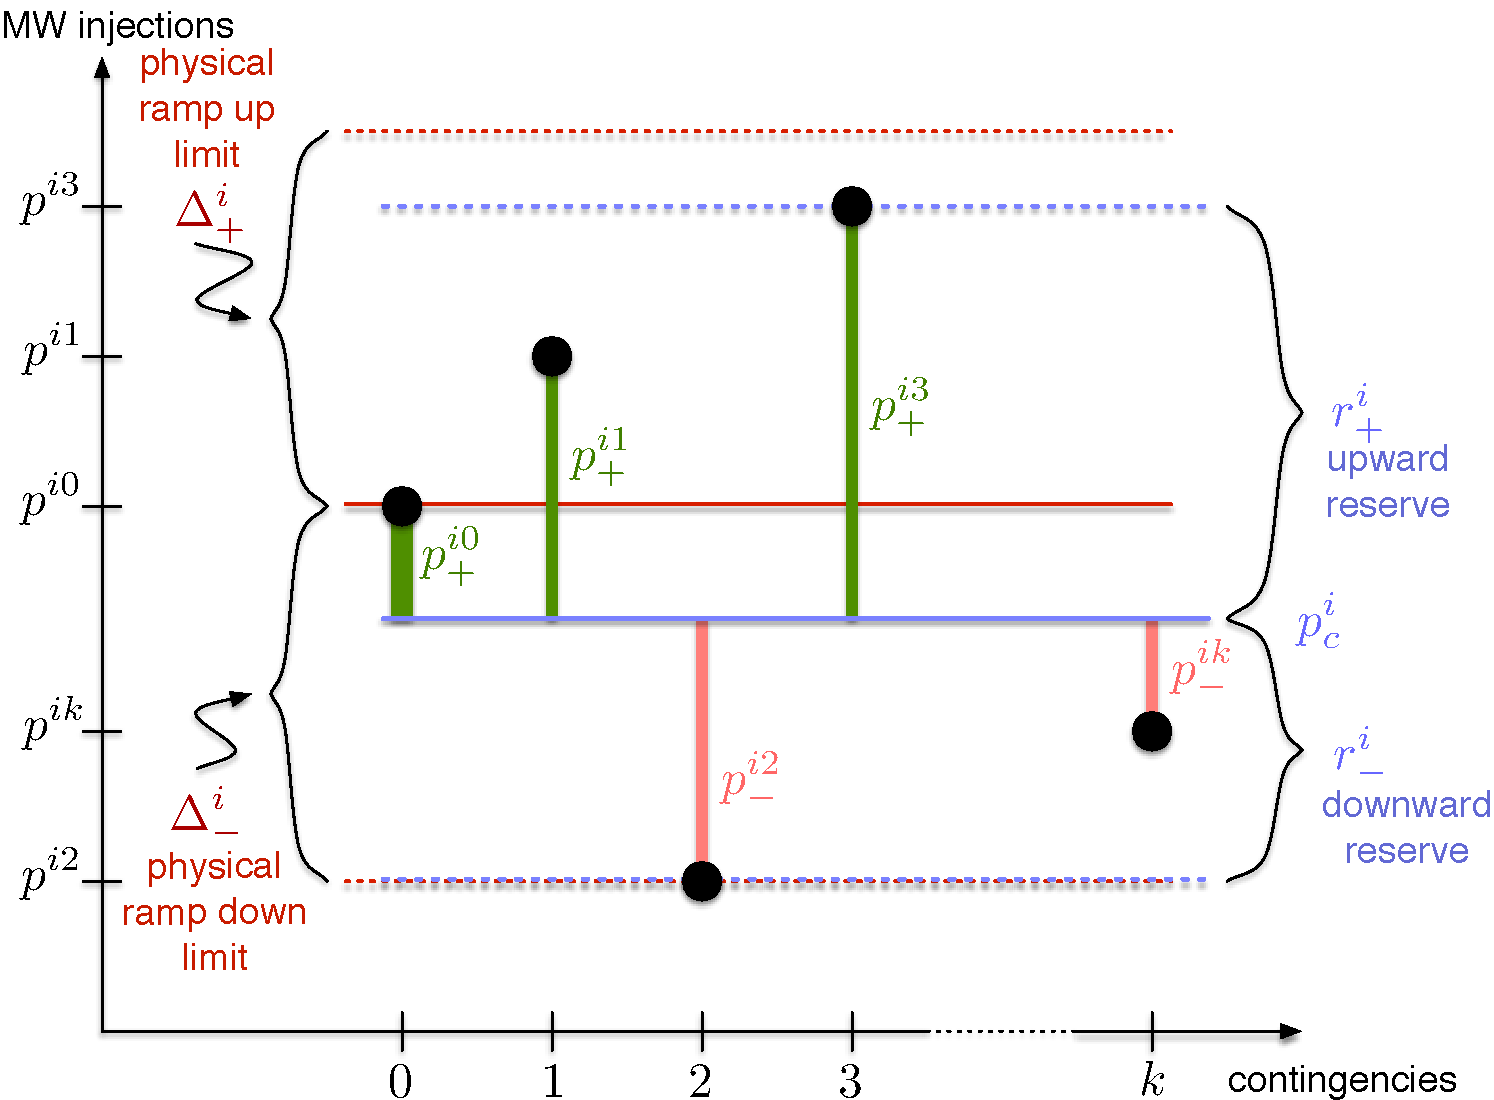
\includegraphics[width=0.8\textwidth]{./figures/reserves-single-base}
  \caption{Reserve Structure for Generator~$i$}
  \label{fig:reserves_single_base}
\end{figure}

Figure~\ref{fig:reserves_single_base} shows the reserve structure for generator~$i$. The green and pink bars show upward and downward redispatches from the reference dispatch $p_c^i$, where the maximums of these deviations define the corresponding reserve quantities. The physical ramp limit restrict deviations of contingency dispatches with respect to the base case dispatch $p^{i0}$.

\subsection{Uncertainty of Demand and Renewable Generation}

While contingencies refer to discrete low probability events, there is another kind of uncertainty introduced by errors in forecasting of demand and renewable sources of generation, such as wind and solar production. This type of uncertainty can be characterized by random system parameters with continuous probability distributions. \most{} can model this type of uncertainty by drawing scenarios from the joint distribution of uncertain parameters and including these scenarios as multiple probability-weighted base cases in a structure similar to that described above for the continencies. There are two primary differences. First, the probabilities of the scenarios used to represent this type of uncertainty need not be small and, second, the base scenarios are tied to each other by the inc/dec and reserve variables, but not by physical ramp limits. This results in a stochastic dispatch problem with endogenously determined generator-specific locational reserves.

To make this problem secure, outage scenarios can be added for each base case, in the same manner as they were added to the single base case problem described previously. For a case with two contingency states, representing uncertain forecasts with two base scenarios results in the problem structure shown in Figure~\ref{fig:structure_multi_scenario}. In this case the reserves are defined by the maximum redispatch deviations across all scenarios and contingencies and the physical ramp rates limit the deviations of contingecy cases from the base case within each scenario, as illustrated in Figure~\ref{fig:reserves}. In this figure the variables include a $t$ index as well, since the same structure is used at each period $t$ in the multiperiod problems discussed below.

\begin{figure}[hbtp]
  \centering
  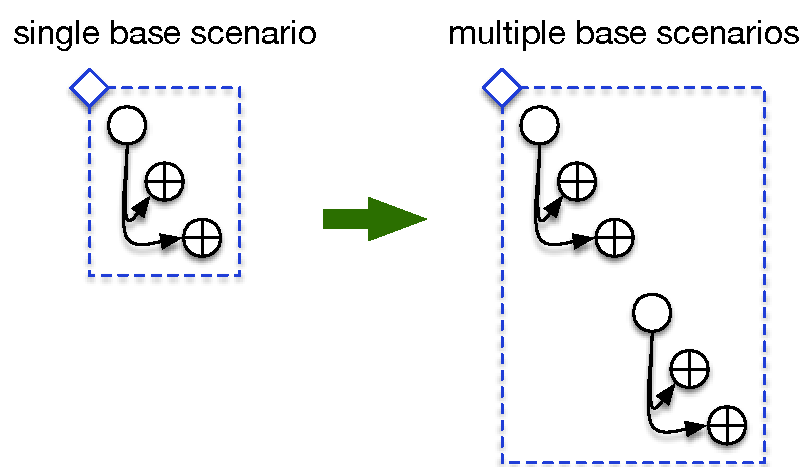
\includegraphics[width=0.5\textwidth]{./figures/structure-multi-scenario}
  \caption{Problem Structure with Multiple Base Scenarios}
  \label{fig:structure_multi_scenario}
\end{figure}

\begin{figure}[hbtp]
  \centering
  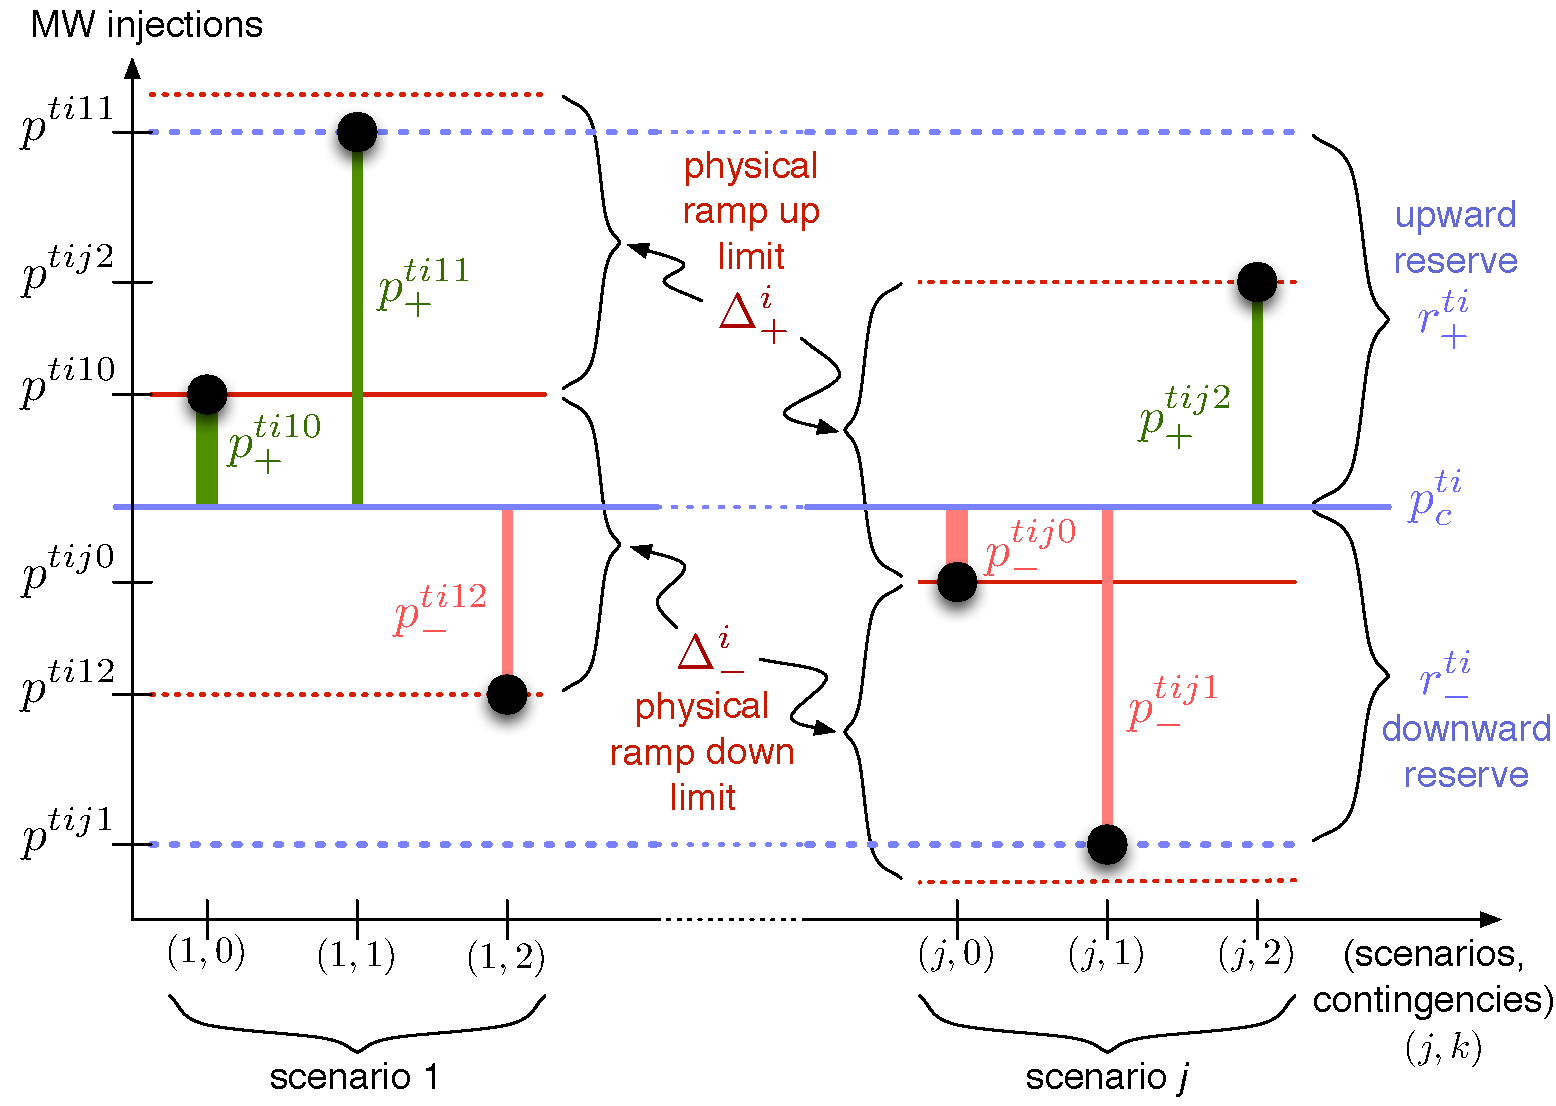
\includegraphics[width=0.8\textwidth]{./figures/reserves}
  \caption{Reserve Structure for Generator~$i$ in Period~$t$}
  \label{fig:reserves}
\end{figure}

Though there are now two types of uncertainty, contingencies and parameter uncertainty for demand and renewables, the reference dispatch and reserve decisions are made before the uncertainty is realized, with the state-specific dispatch decisions being recourse decisions contingent on the revealed outcome of both types of uncertainty.

\subsection{Multiple Periods}

For deterministic scheduling problems, the extension to multiple periods is straightforward. The single period problem is duplicated for each period in the planning horizon and combined into a single large problem which the individual periods appear as islands in a single network. Linking between adjacent periods is in the form of ramping costs and constraints involving the corresponding dispatch variables.

In the case of the stochastic problems with multiple probabilistic system states in each period, the extension to multiple periods is more complicated. One approach is to define each ``scenario'' as a particular realization of all uncertainties, defining a full trajectory through the entire planning horizon. The challenge here is in enforcing the non-anticipativity of the recourse decisions, since in reality the uncertainty is revealed period by period. On the other extreme, the option is to assume that from each scenario in period~$t$ the system might transition to any of a number of states in period~$t+1$. Clearly, the explosion of the number of states with the length of the planning horizon is the barrier to adopting this approach.

\most{} takes this multi-stage decision approach, but adds scenario recombination and scenario trimming to avoid the exploding number of scenarios. This is accomplished by assuming a Markovian structure for a high-probability central path where a transition probability matrix is used to describe the transitions from a limited set of base scenarios in one period to a limited set of base scenarios in the next period. States subsequent to contingency states are trimmed, on the assumption that they occur with low probability and likely require re-optimizing for the future following their occurence.

\subsection{Ramping and Load Following Ramp Reserves}

Ramping feasibility is only enforced on this high probability central path, in which all possible transitions are constrained to be feasible with respect to physical ramping capabilities as well as any load following reserve capacity offers. \most{} includes the facility to define a simple quadratic ``wear and tear'' cost on the difference in dispatch from one period to another, applied in as a probability-weighted cost to each possible transition, as well as up and down load-following ramping reserve costs. These reserve costs apply to maximum upward and downward transitions included in the central path scenarios, as illustrated in Figure~\ref{fig:ramping}.

\begin{figure}[hbt]
  \centering
  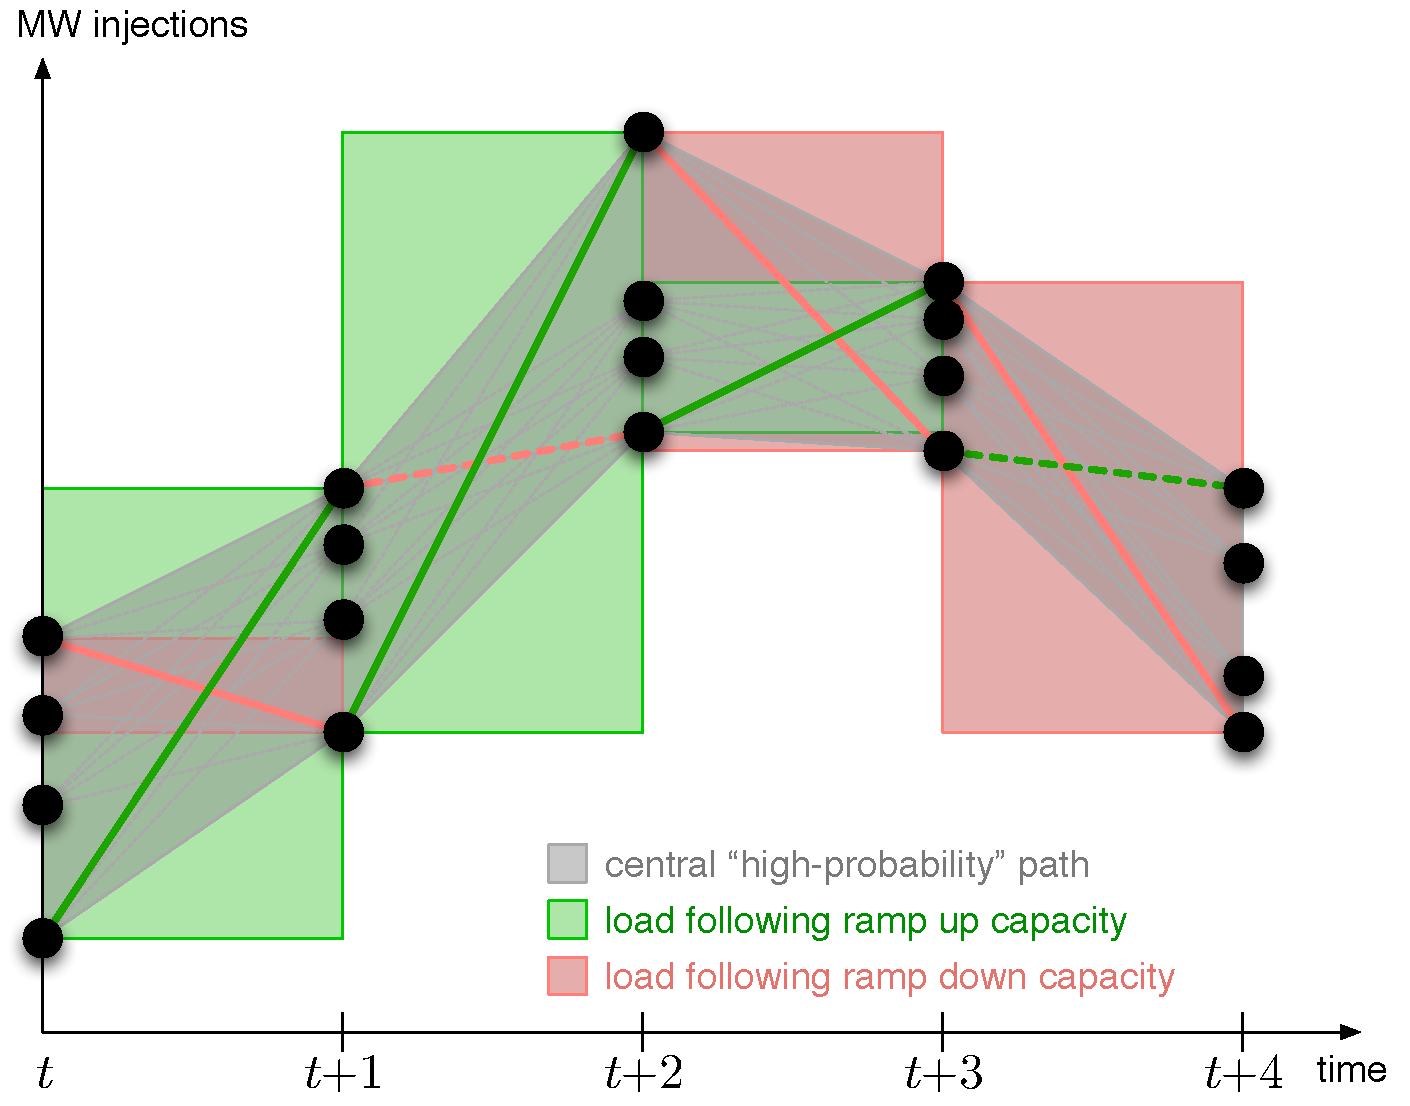
\includegraphics[width=0.8\textwidth]{./figures/ramping-9}
  \caption{Ramping and Load Following Ramp Reserves}
  \label{fig:ramping}
\end{figure}

\subsection{Storage and Deferrable Demand}

Including the time dimension in the problem also opens the door for centrally dispatching resources such as energy storage and deferrable demand technologies which inherently couple operations across time periods. Battery terminology, such as charging and discharging, will be used to describe the storage model implemented by \most{}, though the concepts and model are applicable to a range of storage and energy limited technologies, including batteries, pumped-storage units, combined space conditioning and thermal storage (e.g. ice batteries), and even dispatchable demands or generation with an energy quota over a given horizon.

A storage unit is implemented as a generator with an associated stored energy. The unit has upper and lower bounds on both power and energy, all of which can be either positive or negative. The power bounds define the maximum and minimum power injections, corresponding to the discharging and charging power limits for a traditional battery. The bounds on stored energy, which can vary over time, are used to specify the energy capacity (e.g. for a battery) or quota (e.g. time-flexible demand). The storage unit can also have non-unity charging and discharging efficiencies as well as a loss coefficient defining energy losses in each period as a linear function of the amount of stored energy.

For deterministic problems, as with ramping, enforcing the intertemporal constraints imposed by such an energy storage resource is straightforward. In this case, it is a simple set of conservation of energy constraints.

For the stochastic problems, on the other hand, it becomes more complicated. Since the quantity of stored energy available in any given scenario at time~$t$ is dependent on the dispatches in preceding periods, there is no uniquely defined quantity of stored energy for each scenario, so it is not possible to track actual stored energy values, only expected values and minimum and maximum values.

For this reason \most{} defines decision variables representing the upper and lower bounds on stored energy in each period and enforces feasibility with respect to these limits. Figure~\ref{fig:storage} shows how these limits spread out from period to period when the dispatch of the storage unit varies across scenarios. The only instance in which the limits do not spread out is if the unit adheres to the same dispatch schedule across all scenarios in a period. This formulation allows the optimization problem to make an optimal tradeoff between using the storage to arbitrage energy across time (same dispatch schedule across scenarios to avoid spreading of limits) and using it to mitigate uncertainty (vary the dispatch in response to the different scenarios, but at the expense of spreading limits).

\begin{figure}[tp]
  \centering
  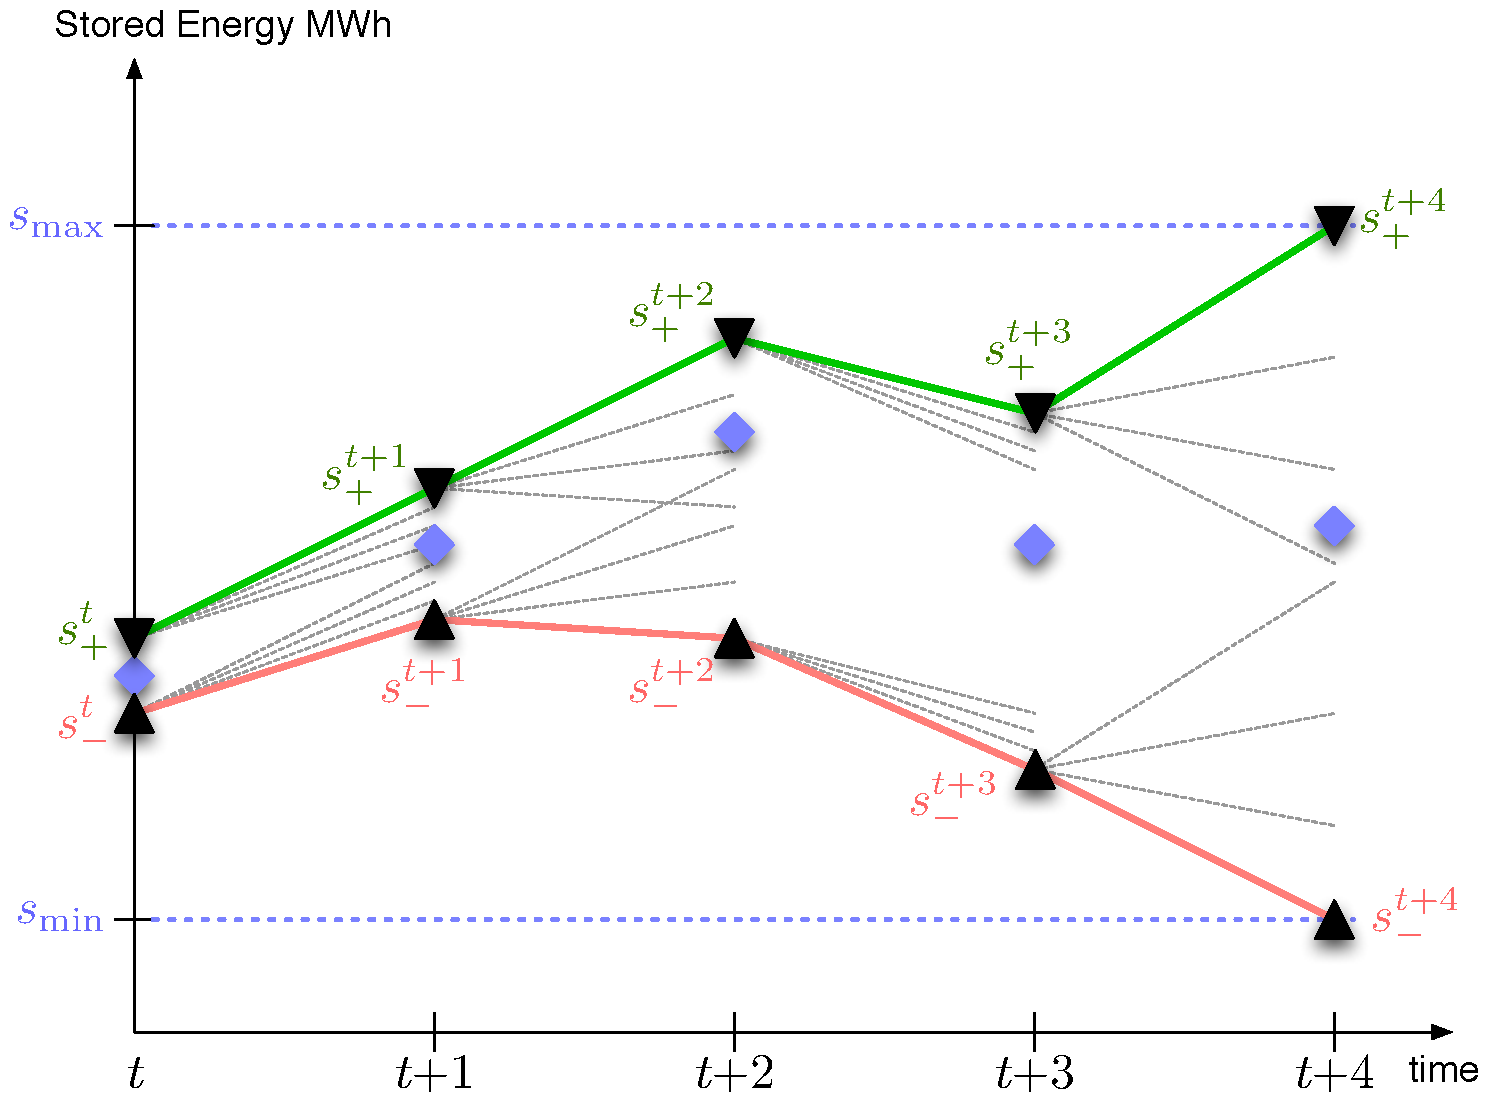
\includegraphics[width=0.8\textwidth]{./figures/storage-18}
  \caption{Storage}
  \label{fig:storage}
\end{figure}

The formulation also includes the option to relax the restrictions on the stored energy bounds in some or all periods to base them on the range of \emph{expected} stored energy quantities in the previous period, rather than on the worst case ranges.

An important aspect of modeling storage is to include some way of either valuing or constraining both the initial amount of stored energy in each unit and the amount of leftover storage in terminal states, both end-of-horizon states and contingency states. \most{} includes several options. First, for each unit there is a cost assigned to any initial stored energy at the beginning of the horizon. Similarly, there are a number of parameters used to specify the value of leftover stored energy in terminal states. Furthermore, the initial stored energy amount can be specified and the final expected stored energy amount can be constrained to equal a target quantity. Finally, there is also the option to simply constrain the initial amount and the final expected amount to be equal while letting that level be determined as an output of the optimization.
 
\subsection{Linear Time-Varying Dynamical System}

The main decision variables in the problem are the dispatches, and they in turn can affect subsequent systems of different kinds.
Specifically, the dispatch schedule can be restricted by putting constraints on the states of a linear time-varying system whose inputs are the expected dispatches at each time period.

One can think, for example, of a very simplified atmospheric diffusion model in which the amount of a greenhouse gas or pollutant released by a specific generation unit is proportional its dispatch.
Or, perhaps the water level at different locations of a river downstream from a hydro unit can be modeled using a linear time-varying system driven by the unit's dispatch history.
Flood levels or navigability might impose constraints on those levels.
While this modeling capability is not, by any means, for the casual user of \most{}, advanced users may find that it provides a flexible mechanism for customization that precludes the need for modifying the \most{} code directly to achieve purpose-specific ends.

\subsection{Unit Commitment}

So far, the discussion has been restricted to problems with continuous optimization variables, with an overall structure for the general case as illustrated in Figure~\ref{fig:structure}.\footnote{The linear dynamical system constraints and the unit commitment aspects of the problem are not included in this illustration.} The class of problems addressed by \most{} also includes those with discrete unit commitment decisions, with optional startup and shutdown costs associated with changes in online status from a prior commitment state. In multiperiod problems, these states are coupled through time, not only by the startup and shutdown costs, but also by minimum up and down time constraints.

\begin{figure}[hbtp]
  \centering
  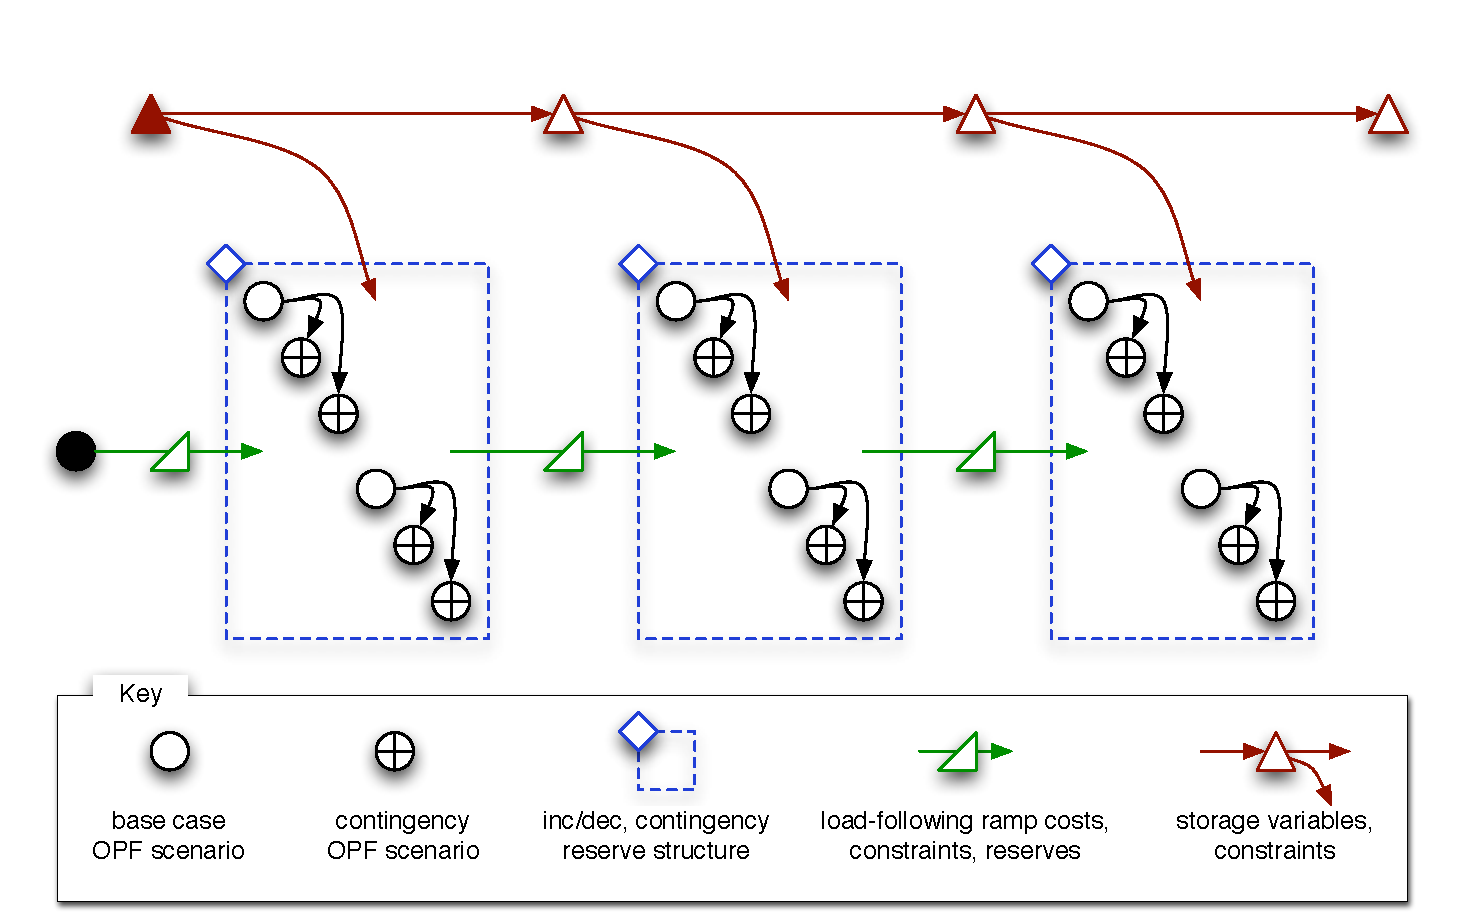
\includegraphics[width=\textwidth]{./figures/structure-multi-period}
  \caption{Overall Problem Structure}
  \label{fig:structure}
\end{figure}

For stochastic problems modeling multiple scenarios and/or contingency states there is a single commitment schedule shared by all states. That is, in the current formulation, a single binary variable is used to model the commitment for a given unit across all scenarios and contingencies in a given period.\footnote{To correctly model the commitment of fast start units with non-zero minimum generation constraints requires individual commitment variables for each scenario.}

Figure~\ref{fig:most_multi_period} illustrates the ways in which any one of the single period continuous variable problems of Figure~\ref{fig:most_single_period} can be extended to include combinations of multiple periods, ramping, storage, integer commitment, startup and shutdown costs and minimum up and down times. 

\begin{figure}[hbtp]
  \centering
  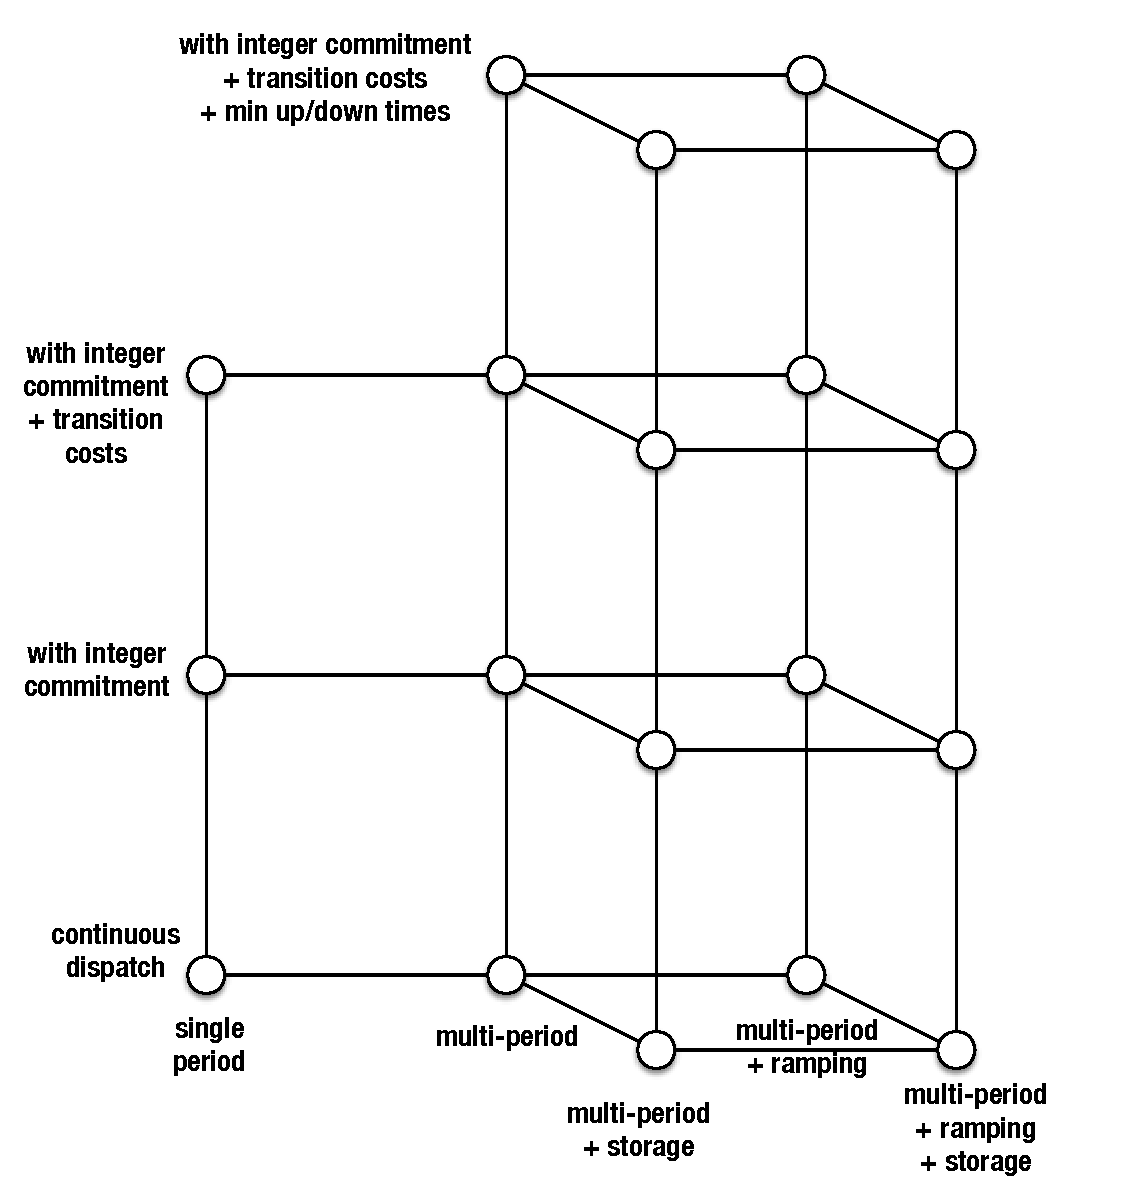
\includegraphics[width=0.8\textwidth]{./figures/most-multi-period-problems-14}
  \caption{MOST Mixed Integer and Multi-Period Problems}
  \label{fig:most_multi_period}
\end{figure}



%%------------------------------------------
\clearpage
\section{Problem Formulation}
\label{sec:probformulation}

%%------------------------------------------
% \clearpage
\subsection{Nomenclature}
\label{sec:nomenclature}

This section summarizes the nomenclature for the full multi-period mixed-integer nonlinear problem. In order to simplify the indexing notation, the index literals and their order are maintained wherever possible. Furthermore, no commas are used, so the superindex $tijk$ refers to time period~$t$, generator~$i$ (or dispatchable load or storage unit~$i$), base scenario~$j$ and contingency~$k$. A dispatchable or curtailable load is modeled as negative generation, as in Section~\ref{MUM-sec:dispatchable_loads} in the \mum{}, each wind farm as a generator whose maximum output varies by scenario according to the forecast distribution, and a storage unit as a device with a given loss factor, energy capacity, and ``charging'' and ``discharging'' power capacities and efficiencies.

\begin{namelist}{XXXXXXXXXX}
\item[]
\item[{\bf Variable and Parameter Indexing}]
\item[\emph{Symbol}] \emph{Meaning}
\item[$t$] Index over time periods.
\item[$T$] Set of indices of time periods in planning horizon, typically $\{ 1\ldots n_t\}$.
\item[$j$] Index over scenarios.
\item[$J^t$] Set of indices of all scenarios considered at time~$t$.
\item[$k$] Index over post-contingency cases ($k = 0$ for base case, i.e. no contingency occured).
\item[$K^{tj}$] Set of indices of contingencies considered in scenario~$j$ at time~$t$, including base case ($k=0$).
\item[$i$] Index over injections (generation units, storage units and dispatchable or curtailable loads).
\item[$I^t$] Indices of all units (generators, storage and dispatchable or curtailable loads) available for dispatch in \emph{any} contingency at time~$t$.
\item[$I^{tjk}$] Indices of all units available for dispatch in post-contingency state~$k$ of scenario~$j$ at time~$t$.
\item[$l$] Index over reserve zones.
\item[$L^{tjk}$] Indices of all reserve zones defined in post-contingency state~$k$ of scenario~$j$ at time~$t$.
\item[$Z_l^{tjk}$] Set of generators providing reserves in zone~$l$ in post-contingency state~$k$ of scenario~$j$ at time~$t$.
\item[$n_t^{\rm ds}$] Number of time periods in the horizon of the dynamical system model.

\item[]
\item[{\bf Optimization Variables}]
\item[\emph{Symbol}] \emph{Meaning}
\item[$p^{tijk}, q^{tijk}$] Active/reactive injection for unit~$i$ in post-contingency state~$k$ of scenario~$j$ at time~$t$.
\item[$p_c^{ti}$] Active power contract quantity for unit~$i$ at time~$t$.
\item[$p_+^{tijk}, p_-^{tijk}$] Upward/downward deviation from active power contract quantity for unit~$i$ in post-contingency state~$k$ of scenario~$j$ at time~$t$.
\item[$r_z^{tijk}$] Zonal reserve quantity provided by unit~$i$ in post-contingency state~$k$ of scenario~$j$ at time~$t$.
\item[$r_+^{ti}, r_-^{ti}$] Upward/downward active contingency reserve quantity provided by unit~$i$ at time~$t$.
\item[$\delta_+^{ti}, \delta_-^{ti}$] Upward/downward load-following ramping reserves needed from unit~$i$ at time $t$ for transition to time $t+1$.
\item[$\theta^{tjk}, V^{tjk}, p^{tjk}, q^{tjk}$] Voltage angles and magnitudes, active and reactive injections for power flow in post-contingency state~$k$ of scenario~$j$ at time~$t$.
\item[$p_{\rm sc}^{tijk}, p_{\rm sd}^{tijk}$] Charge/discharge power injections of storage unit~$i$ in post-contingency state~$k$ of scenario~$j$ at time~$t$.
\item[$s_+^{ti}, s_-^{ti}$] Endogenously computed upper/lower bounds on the energy stored in storage unit~$i$ at the end of period~$t$. For $t = 0$ this is a fixed input parameter representing the bounds at the beginning of the first period.
\item[$s_0^i$] Initial stored energy (expected) in storage unit~$i$.
\item[$u^{ti}$] Binary commitment state for unit~$i$ in period~$t$, 1 if unit is on-line, 0 otherwise.
\item[$v^{ti}, w^{ti}$] Binary startup and shutdown states for unit~$i$ in period~$t$, 1 if unit has a startup/shutdown event in period~$t$, 0 otherwise.
\item[$z^t$] Partition ($n_z^{\rm ds} \times 1$ vector) corresponding to period~$t$ of state variable $z$ of the dynamical system model.

\item[]
\item[{\bf Constraint Functions and Parameters}]
\item[\emph{Symbol}] \emph{Meaning}
\item[$g^{tjk}(\cdot)$] Nonlinear AC power flow equations in post-contingency state~$k$ of scenario~$j$ at time~$t$.
\item[$h^{tjk}(\cdot)$] Transmission, voltage and other limits in post-contingency state~$k$ of scenario~$j$ at time~$t$.
\item[$P_{\rm min}^{tijk}, P_{\rm max}^{tijk}$] Limits on active injection for unit~$i$ in post-contingency state~$k$ of scenario~$j$ at time~$t$.
\item[$Q_{\rm min}^{tijk}, Q_{\rm max}^{tijk}$] Limits on reactive injection for unit~$i$ in post-contingency state~$k$ of scenario~$j$ at time~$t$.
\item[$R_{\rm max+}^{ti}, R_{\rm max-}^{ti}$] Upward/downward contingency (or zonal) reserve capacity limits for unit~$i$ at time~$t$.
\item[$R_l^{tjk}$] MW reserve requirement for zone~$l$ in post-contingency state~$k$ of scenario~$j$ at time~$t$.
\item[$\delta^{ti}_{\rm max+}, \delta^{ti}_{\rm max-}$] Upward/downward load-following ramping reserve limits for unit~$i$ at time $t$ for transition to time $t+1$.
\item[$\Delta_+^i, \Delta_-^i$] Upward/downward physical ramping limits for unit~$i$ for transitions from base ($k=0$) to contingency cases.
\item[$\rho^{ti}$] Parameter for storage unit~$i$ at period $t$ that determines the weighting in storage constraints, where the storage dispatch bounds are computed relative to a weighted average of previous period endogenous bounds $s_+^{(t-1)i}$, $s_-^{(t-1)i}$ ($\rho^{ti} = 1$) and period- and scenario-specific initial expected stored energy ($\rho^{ti} = 0$).
\item[$S^{ti}_{\rm max},S^{ti}_{\rm min}$] Stored energy (in MWh) max/min limits for storage unit~$i$ at time~$t$.
\item[$S_{\rm min}^{0i}$, $S_{\rm max}^{0i}$] Lower/upper bounds on initial stored energy (expected) in storage unit~$i$.
\item[$S_{\rm min}^{n_ti}$, $S_{\rm max}^{n_ti}$] Lower/upper bounds on target stored energy (expected) in storage unit~$i$ at end of final period~$n_t$.
\item[$\tau_i^+, \tau_i^-$] Minimum up and down times for unit~$i$ in number of periods.
\item[$A_{\rm ds}^t, B_{\rm ds}^t, C_{\rm ds}^t, D_{\rm ds}^t$] Matrices used to define the state transitions and output constraints for the dynamical system model at time~$t$.
\item[$z_{\rm min}^t, z_{\rm max}^t$] Lower and upper bounds on dynamical system model state $z^t$ at time~$t$.
\item[$y_{\rm min}^t, y_{\rm max}^t$] Lower and upper bounds on dynamical system model output at time~$t$.

\item[]
\item[{\bf Cost Functions and Parameters}]
\item[\emph{Symbol}] \emph{Meaning}
\item[$C_P^{ti}(\cdot)$] Cost function for active injection~$i$ at time~$t$.
\item[$C_{P+}^{ti}(\cdot), C_{P-}^{ti}(\cdot)$] Cost for upward/downward deviation from active power contract quantity for unit~$i$ at time~$t$.
\item[$C_z^{ti}(\cdot)$] Cost function for zonal reserve purchased from unit~$i$ at time~$t$.
\item[$C_{R+}^{ti}(\cdot), C_{R-}^{ti}(\cdot)$] Cost function for upward/downward contingency reserve purchased from unit~$i$ at time~$t$.
\item[$C_{\delta+}^{ti}(\cdot),C_{\delta-}^{ti}(\cdot)$] Cost of upward/downward load-following ramp reserve for unit~$i$ at time~$t$ for transition to time $t+1$.
\item[$C_\delta^i(\cdot)$] Quadratic, symmetric ramping cost on the difference between the dispatches for unit~$i$ in adjacent periods.
\item[$C_{s0}$] Vector of costs by storage unit associated with starting out with a given level of stored energy $s_0$ in the storage units at time $t=0$.
\item[$C_{s}$] Vector of prices by storage unit for contributions to terminal storage\footnote{That is, expected leftover stored energy in terminal states.}  from charging or discharging in non-terminal states.
\item[$C_{\rm sc0}, C_{\rm sd0}$] Vector of prices by storage unit for contributions to terminal storage\footnotemark[\value{footnote}] from charging/discharging in terminal end-of-horizon base states.
\item[$C_{{\rm sc}k}, C_{{\rm sd}k}$] Vector of prices by storage unit for contributions to terminal storage\footnotemark[\value{footnote}] from charging/discharging in terminal contingency states.
\item[$C_v^{ti}, C_w^{ti}$] Startup and shutdown costs for unit~$i$ at time~$t$ in \$ per startup/shutdown.

\item[]
\item[{\bf Other Parameters}]
\item[\emph{Symbol}] \emph{Meaning}
\item[$\Delta$] Length of scheduling time slice in hours, typically 1~hour.
\item[$\eta^{ti}_{\rm in}, \eta^{ti}_{\rm out}$] Charging/discharging (or pumping/generating) efficiencies for storage unit~$i$ at time~$t$.
\item[$\eta^{ti}_{\rm loss}$] Fraction of stored energy lost per hour by storage unit~$i$ at time~$t$.
\item[$\alpha$] For contingency cases, the fraction of the time slice that is spent in the base case before the contingency occurs ($\alpha = 0$ means the entire period is spent in the contingency).
\item[$\psi_0^{tjk}$] Conditional probability of contingency~$k$ in scenario~$j$ at time~$t$, conditioned on making it to period~$t$ without branching off the central path in a contingency in periods $1\ldots t-1$ and on scenario~$j$ being realized in some form (base or contingency). $\psi_0^{tj0}$ is the conditional probability of no contingency, i.e. the base case.
\item[$\phi^{tj_2j_1}$] Probability of transitioning to scenario $j_2$ in period~$t$ given that scenario $j_1$ was realized in period $t-1$.
\item[$\zeta^{tj_2j_1}$] Binary valued mask indicating whether transition to scenario $j_2$ in period~$t$ from scenario $j_1$ in period $t-1$ should be included in load-following ramp requirements.

\item[]
\item[{\bf Derived Parameters}]
\item[\emph{Symbol}] \emph{Meaning}
\item[$\widetilde{C}_P^{ti}(\cdot)$] Modified cost function for active injection~$i$ at time~$t$ with the no load cost subtracted, $\widetilde{C}_P^{ti}(p) \equiv C_P^{ti}(p) - C_P^{ti}(0)$.
\item[$C_{\rm ts0}, C_{\rm tsc}, C_{\rm tsd}$] Weighted price vectors summarizing contributions to the value of terminal storage\footnotemark[\value{footnote}] from initial storage/charging/discharging, derived from $C_{s}$, $C_{\rm sc0}$, $C_{\rm sd0}$, $C_{{\rm sc}k}$, $C_{{\rm sd}k}$.\footnote{See Section~\ref{sec:residualstorage}, especially \eqref{eq:fs}--\eqref{eq:Ctsd}, for details.}
\item[$\psi^{tjk}$] Probability of contingency~$k$ in scenario~$j$ at time~$t$, derived from transition probabilities $\phi^{tj_2j_1}$ and conditional probabilities of contingencies $\psi_0^{tjk}$. $\psi^{tj0}$ is the probability of no contingency, i.e. the base case.
\item[$\psi_\alpha^{tjk}$] Probability $\psi^{tjk}$ of contingency~$k$ in scenario~$j$ at time~$t$ adjusted for $\alpha$. \\
                \begin{equation}
                    \psi_\alpha^{tjk} = \left\{\begin{aligned}
                        && \psi^{tj0} + \alpha \!\!\! \sum_{\kappa \in K^{tj} \ne 0} \psi^{tj\kappa}, &&& k = 0 \\
                        && (1-\alpha) \psi^{tjk}, &&& \forall k \in K^{tj} \ne 0
                    \end{aligned}\right.
                    \label{eq:psialpha}
                \end{equation}
\item[$\gamma^t$] Probability of making it to period~$t$ without branching off the central path in a contingency in periods $1\ldots t-1$.
\begin{equation}
\gamma^t \equiv \!\! \sum_{j \in J^{t-1}} \psi^{(t-1)j0} = \!\!\!\!\! \sum_{j \in J^t, k \in K^{tj}} \!\!\! \psi^{tjk}
\end{equation}
\item[$\beta_1^{ti}$ \dots $\beta_5^{ti}$] Storage parameters defined in \eqref{eq:beta1and2} and \eqref{eq:beta3}--\eqref{eq:beta5} in terms of $\Delta$, $\alpha$ and $\eta^{ti}_{\rm loss}$ to simplify storage constraint expression.


\item[]
\item[{\bf Derived Variables}]\footnote{All are linear functions of the optimization variables, used only to simplify the presentation.}
\item[\emph{Symbol}] \emph{Meaning}
\item[$s_\Delta^{tijk}$] Net increase in stored energy due to charging or discharging for unit~$i$ in post-contingency state~$k$ of scenario~$j$ at time~$t$.
\begin{equation}
s_\Delta^{tijk} \equiv - \Delta(\eta^{ti}_{\rm in} p^{tijk}_{\rm sc} + \frac{1}{\eta^{ti}_{\rm out}} p_{\rm sd}^{tijk}) \label{eq:sdelta}
\end{equation}
\item[$\bar{S}_I^{tj}$] Vector of expected stored energy for all storage units in base scenario~$j$ at the beginning of period~$t$, defined as a linear function of $s_0$, $p_{\rm sc}$ and $p_{\rm sd}$.\footnote{See Section~\ref{sec:residualstorage} for details.}
% , described in the paragraph preceding \eqref{eq:SFntj}
\item[$\bar{s}_I^{tij0}$] Expected stored energy in storage unit~$i$ in base scenario~$j$ at the beginning of period~$t$ ($i$-th element of $\bar{S}_I^{tj}$).
\item[$s_F^{n_ti}$] Expected stored energy in storage unit~$i$ at the end of period $n_t$, the final period.\footnotemark[\value{footnote}]
\item[$\bar{p}^t$] Vector of expected values of $p^{tijk}$ across $j$ and $k$ at time~$t$, conditional on making it to time~$t$.
\begin{equation}
 \bar{p}^t = \frac{1}{\gamma^t} \sum_{j \in J^t, k \in K^{tj}} \!\!\! \psi_\alpha^{tjk} p^{tjk} \label{eq:expected_dispatch}
\end{equation}


\end{namelist}
Individual variables can be grouped into vectors such as $p^{t}$ for all active injections considered across all scenarios and contingencies at hour $t$ and it will be consistent with the context. The subset referring to scenario~$j$ would be $p^{tj}$.
%Injections related to unit~$i$ for all time periods would be denoted by $p^{Ti}$, and the subset of these related only to all root cases would be $p^{TiJ0}$, since $k=0$ refers to a root case.

%%------------------------------------------
\clearpage
\subsection{Formulation}
\label{sec:formulation}

The problem formulation can be expressed as a mixed-integer nonlinear optimization problem, where the optimization variable $x$ is comprised of all the $\theta$, $V$, $p$, $q$, $p_c$, $p_+$, $p_-$, $r_z$, $r_+$, $r_-$, $\delta_+$, $\delta_-$, $p_{\rm sc}$, $p_{\rm sd}$, $s_0$, $s_+$, $s_-$, $u$, $v$, $w$, and $z$ variables, for all $t$, $j$, $k$, $i$ and $l$. The $u$ commitment variables are binary and the rest continuous. For simplicity, the formulation restricts the treatment of costs, deviations, ramping and reserves to consider only active power, but an extension to include reactive counterparts is straightforward.

\subsubsection{Objective Function}

The objective then is to
\begin{equation}
\min_x f(x)
\label{eq:objfcn1}
\end{equation}
where $f(x)$ is comprised of seven components.\footnote{A typical secure problem uses either zonal reserves or endogenous contingency reserves, but not both. Zonal reserves are typically used only for cases with a single base scenario with no contingencies, that is, when $J^t = \{1\}$ and $K^{tj} = \{0\}$.}
\begin{align}
f(x) = \;& f_p(p,p_+,p_-) + f_z(r_z) + f_r(r_+, r_-) + f_\delta(p) \nonumber \\
    &{} + f_{\rm lf}(\delta_+, \delta_-)
     + f_s(s_0, p_{\rm sc}, p_{\rm sd}) + f_{\rm uc}(u,v,w) \label{eq:mostobjective}
\end{align}
Each part is expressed in terms of the individual optimization variables as follows.
\begin{itemize}
\item[--] expected cost of active power dispatch and redispatch
\end{itemize}
\begin{align}
f_p(p,p_+,p_-) &= \sum_{t\in T} \sum_{j\in J^t} \sum_{k\in K^{tj}} \psi_\alpha^{tjk} \sum_{i\in I^{tjk}}
    \Bigl[\widetilde{C}_P^{ti}(p^{tijk}) + C_{P+}^{ti}(p_+^{tijk}) + C_{P-}^{ti}(p_-^{tijk}) \Bigr]
\label{eq:most_energy_cost}
\end{align}
\begin{itemize}
\item[--] cost of zonal reserves\footnotemark[\value{footnote}]
\begin{equation}
f_z(r_z) = \sum_{t\in T} \sum_{j\in J^t} \sum_{k\in K^{tj}} \psi_\alpha^{tjk} \sum_{i\in I^{tjk}} C_z^{ti}(r_z^{tijk})
\label{eq:most_zres_cost}
\end{equation}
\item[--] cost of endogenous contingency reserves\footnotemark[\value{footnote}]
\begin{equation}
f_r(r_+, r_-) = \sum_{t\in T}  \gamma^t  \sum_{i\in I^t} \left[C_{R+}^{ti}(r_+^{ti}) + C_{R-}^{ti}(r_-^{ti}) \right]
\label{eq:most_cres_cost}
\end{equation}
\item[--] expected cost of load-following ramping (wear and tear)
\begin{equation}
f_\delta(p) = \sum_{t\in T} \! \gamma^t \!\!\!\!\! \sum_{\begin{aligned}\scriptstyle j_1 &\scriptstyle \in J^{t-1}\\[-6pt] \scriptstyle j_2 &\scriptstyle \in J^t\end{aligned}} \!\!\!\!\!
        \phi^{t j_2 j_1} \!\!\!\! \sum_{i\in I^{tj_2 0}} \!\!\! C_\delta^i(p^{tij_20} - p^{(t-1)ij_10})
\label{eq:rampcost}
\end{equation}
\item[--] cost of load-following ramp reserves
\begin{equation}
f_{\rm lf}(\delta_+, \delta_-) = \sum_{t\in T}  \gamma^t  \sum_{i\in I^t} \left[C_{\delta+}^{ti}(\delta_+^{ti}) + C_{\delta-}^{ti}(\delta_-^{ti}) \right]
\label{eq:most_rampres_cost}
\end{equation}
\item[--] cost of initial stored energy and value (since it is negative) of expected leftover stored energy in terminal states
\begin{equation}
f_s(s_0, p_{\rm sc}, p_{\rm sd}) = \trans{C_{s0}} s_0 - (\trans{C_{\rm ts0}} s_0 + \trans{C_{\rm tsc}} p_{\rm sc} + \trans{C_{\rm tsd}} p_{\rm sd}) \label{eq:storagecost}
\end{equation}
\item[--] no load, startup and shutdown costs
\begin{equation}
f_{\rm uc}(u,v,w) = \sum_{t\in T} \gamma^t \sum_{i\in I^t} \Bigl( C_P^{ti}(0) u^{ti} + C_v^{ti} v^{ti} +  C_w^{ti} w^{ti} \Bigr)
\end{equation}
\end{itemize}

\subsubsection{Constraints}

This minimization is subject to the following constraints, for all $t \in T$, all $j \in J^t$, all $k \in K^{tj}$, all $i \in I^{tjk}$, and all $l \in L^{tjk}$, beginning with the constraints that are separable by period.

\subsubsection*{Standard OPF Constraints}

\begin{itemize}
\item[--] power balance equations\footnote{These can take the form of nonlinear AC power balance equations \emph{(not yet implemented)} \eqref{MUM-eq:acpf_p} and \eqref{MUM-eq:acpf_q}, linear DC power balance equations \eqref{MUM-eq:dcopf_eq}, or a simple equating of total demand and total supply, where the equation numbers referenced are from the \mum{}.}
\begin{equation}
  g^{tjk}(\theta^{tjk},V^{tjk},p^{tjk},q^{tjk}) = 0 \label{eq:firstopf}
\end{equation}
\item[--] transmission flow limits, voltage limits, any other OPF inequality constraints\footnote{These can also take the form of inequality constraints from a nonlinear AC OPF \emph{(not yet implemented)} including \eqref{MUM-eq:acopf_ieqf}, \eqref{MUM-eq:acopf_ieqt} and \eqref{MUM-eq:vlims}, a linear DC OPF including \eqref{MUM-eq:dcopf_ieqf} and \eqref{MUM-eq:dcopf_ieqt}, or a simple economic dispatch, where the equation numbers referenced are from the \mum{}.}
\begin{equation}
  h^{tjk}(\theta^{tjk},V^{tjk},p^{tjk},q^{tjk}) \leq 0
\end{equation}
% \item[--] injection and other limits (and perhaps more complex generator capability curves
%    or constant power factor constraints for dispatchable loads)
% \begin{eqnarray}
%  P_{\rm min}^{tijk}  & \leq p^{tijk} \leq & P_{\rm max}^{tijk} \label{eq:pbounds} \\
%  Q_{\rm min}^{tijk}  & \leq q^{tijk} \leq & Q_{\rm max}^{tijk} \label{eq:qbounds} \\
%  V_{\rm min}^i &  \leq V^{tijk} \leq  & V_{\rm max}^i   \label{eq:lastopf}
%  \end{eqnarray}
\end{itemize}

% Using \subsubsection*{} below causes problems for building MATPOWER-manual.tex with \externaldocument links to MOST-manual.aux
\noindent{\bf Security Constraints (Option 1): Zonal Reserve Requirements}\footnote{A typical secure problem uses either zonal reserves or endogenous contingency reserves, but not both. Zonal reserves are typically used only for cases with a single base scenario with no contingencies, that is, when $J^t = \{1\}$ and $K^{tj} = \{0\}$.}

\begin{itemize}
\item[--] fixed zonal reserve requirements
\begin{align}
0 \le r_z^{tijk} &\le \min(R_{\rm max+}^{ti}, \Delta_+^i) \label{eq:reserve_var2} \\
p^{tijk} + r_z^{tijk} &\le u^{ti} P_{\rm max}^{tijk} \label{eq:Pg_plus_R2} \\
\sum_{i \in Z_l^{tjk}} r_z^{tijk} &\ge R_l^{tjk} \label{eq:reserve_req2}
\end{align}
\end{itemize}

% Using \subsubsection*{} below causes problems for building MATPOWER-manual.tex with \externaldocument links to MOST-manual.aux
\noindent{\bf Security Constraints (Option 2): Contingency Constraints}\footnotemark[\value{footnote}]
\begin{itemize}
\item[--] reserve, redispatch and contract variables
\begin{eqnarray}
 & &  0 \leq p_+^{tijk} \leq r_+^{ti} \leq R_{\rm max+}^{ti} \label{eq:firstinterflow}\label{eq:maxresp} \\
 & &  0 \leq p_-^{tijk} \leq r_-^{ti} \leq R_{\rm max-}^{ti} \label{eq:maxresm} \\
 & &  p^{tijk} - p_c^{ti} = p_+^{tijk} - p_-^{tijk}
\end{eqnarray}
\item[--] ramping limits on transitions from base to contingency cases
\begin{equation}
   -\Delta_-^i \leq p^{tijk} -p^{tij0} \leq \Delta_+^i, \quad k \neq 0
   \label{eq:lastnonintertemp}
\end{equation}
\end{itemize}

% Let us denote the set of feasible $(p,p_+,p_-,r_+,r_-)$ at time~$t$, described by the previous constraints, as ${\cal S}^t$.
%, so that $(p^t,p_+^t,p_-^t,r_+^t,r_-^t) \in {\cal S}^t$ meets~\eqref{eq:firstnonintertemp}--\eqref{eq:lastnonintertemp}.

The remaining sets of constraints include intertemporal restrictions and typically include constraints from a known starting point at $t=0$ into the first period.

\subsubsection*{Load-following Ramping Limits and Reserves}
\begin{itemize}
\item[--]  variable limits
\begin{align}
0 \leq \delta_+^{ti} &\leq  \delta^{ti}_{\rm max+} \label{eq:deltapbounds} \\
0 \leq \delta_-^{ti} &\leq  \delta^{ti}_{\rm max-}  \label{eq:deltambounds}
\end{align}
\item[--] load-following ramp reserve definition
\begin{align}
\forall \{t \in T, i \in I^{tjk}, j_1 \in J^{t-1}, j_2 &\in J^t \mid \zeta^{tj_2j_1} = 1 \}: \label{eq:rampconstrdef} \\
p^{tij_20} - p^{(t-1)ij_10} &\leq \delta_+^{(t-1)i} \label{eq:inter1} \\
p^{(t-1)ij_10} - p^{tij_20} &\leq \delta_-^{(t-1)i} \label{eq:rampconstr}
\end{align}
\end{itemize}
%Here, the $j_1$ and $j_2$ indices address the need to limit the ramping rate, for example, from a high wind output base case at time~$t$ to a low wind output case at time $t+1$.

\subsubsection*{Storage Constraints}
\begin{itemize}
\item[--] storage dispatch definition and limits
\begin{align}
p^{tijk} &= p^{tijk}_{\rm sc} + p^{tijk}_{\rm sd} \\
p^{tijk}_{\rm sc} &\leq 0 \\
p^{tijk}_{\rm sd} &\geq 0
\end{align}

\item[--] energy bound limits
\begin{align}
s_-^{ti} &\geq S^{ti}_{\rm min} \\
s^{ti}_+ &\leq S^{ti}_{\rm max}
\end{align}

\item[--] storage dispatch vs. base scenario energy bounds
\begin{align}
s^{ti}_- &\leq \beta_1^{ti} \left[\rho^{ti} s^{(t-1)i}_- + \left(1-\rho^{ti}\right) \bar{s}_I^{tij0}\right] + \beta_2^{ti} s_\Delta^{tij0} \label{eq:storage1st} \\
s^{ti}_+ &\geq \beta_1^{ti} \left[\rho^{ti} s^{(t-1)i}_+ + \left(1-\rho^{ti}\right) \bar{s}_I^{tij0}\right] + \beta_2^{ti} s_\Delta^{tij0}
\end{align}

\item[--] storage dispatch vs. contingency scenario energy limits
\begin{align}
S^{ti}_{\rm min} &\leq \beta_5^{ti} \left[\rho^{ti} s^{(t-1)i}_- + \left(1-\rho^{ti}\right) \bar{s}_I^{tij0}\right] + \beta_4^{ti} s_\Delta^{tij0} + \beta_3^{ti} s_\Delta^{tijk}, \;\; k\neq 0 \\
S^{ti}_{\rm max} &\geq \beta_5^{ti} \left[\rho^{ti} s^{(t-1)i}_+ + \left(1-\rho^{ti}\right) \bar{s}_I^{tij0}\right] + \beta_4^{ti} s_\Delta^{tij0} + \beta_3^{ti} s_\Delta^{tijk}, \;\; k\neq 0
\label{eq:storagecontingencylast}
\end{align}

\item[--] optional storage constraints
\begin{itemize}

\item[--] Option 1 : Constrain the expected final stored energy in each unit at the end of the horizon\footnote{See \eqref{eq:sfend} in the Section~\ref{sec:residualstorage} for details on how $s_F^{n_ti}$ is computed as a linear function of $x$.} to equal some target value or lie in some target range.
\begin{equation}
S_{\rm min}^{n_ti} \le s_F^{n_ti} \le S_{\rm max}^{n_ti} \label{eq:sftarget}
\end{equation}
\item[--] Option 2 : Constrain the expected final stored energy at the end of the horizon\footnotemark[\value{footnote}] to equal the initial stored energy.
\begin{align}
s_F^{n_ti} &= s_0^i \label{eq:sfequals0} \\
S_{\rm min}^{0i} &\le s_0^i \le S_{\rm max}^{0i} \label{eq:s0bounds}
\end{align}
When using this option $s_0^i$ is an optimization variable that can take on any value between its bounds. When not using this option, it is simply a fixed parameter.
\end{itemize}

\end{itemize}

\subsubsection*{Unit Commitment}
\begin{itemize}
\item[--] injection limits and commitments
\begin{align}
 u^{ti} P_{\rm min}^{tijk} & \leq p^{tijk} \leq u^{ti} P_{\rm max}^{tijk} \\
 u^{ti} Q_{\rm min}^{tijk} & \leq q^{tijk}  \leq u^{ti} Q_{\rm max}^{tijk}
\end{align}
\item[--] startup and shutdown events
\begin{align}
 u^{ti} - u^{(t-1)i} &= v^{ti} - w^{ti} \\
 0 \le v^{ti} &\le 1 \\
 0 \le w^{ti} &\le 1
\end{align}
\item[--] minimum up and down times
\begin{align}
 \sum_{y=t-\tau_i^+ + 1}^t v^{yi} & \le u^{ti} \\
 \sum_{y=t-\tau_i^- + 1}^t w^{yi} & \le 1 - u^{ti}
\end{align}
Note: These summations can be made to ``wrap around'' to implement a cyclic commitment schedule where commitment transitions from the last period of the horizon back to the first are also constrained to be feasible.
\item[--] integrality constraints
\begin{equation}
u^{ti} \in \{0,1\}
\end{equation}
\end{itemize}

\subsubsection*{Linear Time-Varying Dynamical System}

The partition of the state variable corresponding to time~$t$ is denoted $z^t$, the corresponding output by $y^t$ (not an explicit optimization variable), and $\bar{p}^t$ represents the vector of expected values of $p^{tijk}$ across $j$ and $k$ at time~$t$, conditional on making it to time~$t$, as defined in \eqref{eq:expected_dispatch}. That is
\begin{equation}
 \bar{p}^t = \frac{1}{\gamma^t} \sum_{j \in J^t, k \in K^{tj}} \!\!\! \psi_\alpha^{tjk} p^{tjk}
\end{equation}
\begin{itemize}
\item[--] state bounds
\begin{align}
 z_{\rm min}^t & \leq z^t \leq  z_{\rm max}^t, & t &= 1 \dots n_t^{\rm ds} \label{eq:dynbounds}
\end{align}
\item[--] state update equations
\begin{align}
 z^{t+1} & = A_{\rm ds}^t z^t + B_{\rm ds}^t \bar{p}^t, & t &= 1 \dots n_t \label{eq:dynstate1} \\
 z^{t+1} & = A_{\rm ds}^t z^t, & t &= (n_t + 1) \dots (n_t^{\rm ds}-1) \label{eq:dynstate2}
\end{align}
\item[--] output equations
\begin{align}
 y_{\rm min}^t & \le C_{\rm ds}^t z^t + D_{\rm ds}^t \bar{p}^t \le y_{\rm max}^t, & t &= 1 \dots n_t \label{eq:dynout1} \\
 y_{\rm min}^t & \le C_{\rm ds}^t z^t \qquad\quad\; \le y_{\rm max}^t, & t &= (n_t + 1) \dots n_t^{\rm ds} \label{eq:dynout2}
\end{align}
\end{itemize}
The initial state $z^1$ is not a variable, but is assumed to be a given initial condition.

\subsection{Probability Weighting of Base and Contingency States}

This section describes the assumptions regarding the probabilistic weighting of each term in the cost function. A given initial state at time $t=0$, with known dispatches and energy storage states, is assumed to have probability 1. From this initial state, transitions, each with some known probability, are possible to any of the scenarios considered for period $t=1$. Hence the probabilities assigned to each of the states in period $t=1$ sum to 1.

Now, consider the transition into $t=2$. This transition is only possible provided the system did not branch off into any contingency at time $t=1$, that is, provided the realized state at $t=1$ is one of the base scenarios. However, given that at least one contingency has a non-zero probability of occurrence, the sum of the probabilities of these base cases for $t=1$ is less than 1. So the probability of actually making it to $t=2$ in the considered graph is equal to the sum of the probabilities of the base cases at $t=1$, which is less than 1. Generalizing for period~$t$, the probability of making it to period~$t$ is equal to the sum of the probabilities of the base cases at $t-1$, a value less than 1 except when $t=1$:

\begin{equation}
\gamma^t = \sum_{j \in J^t} \psi^{(t-1)j0} = \sum_{j \in J^t, k \in K^{tj}} \psi^{tjk} < 1,\;\; t>1
\end{equation}

While the fact that the probabilities in future periods do not sum to 1 may seem odd, this results from choosing, in an $N-1$ contingency fashion, to ignore the cost implications of resuming normal operations after branching off in a contingency, since that would involve exploration of a geometric number of possible paths. This implies, for the branches that have been trimmed, the existence of an unknown cost with respect to the decision variables. Since we do not have any information about the relationship of this unknown cost to our decisions, we explicitly ignore its impact by excluding it from the optimization.

The probability of transitioning to scenario $j_2$ in period~$t$ given that scenario $j_1$ was realized in period $t-1$ is assumed to be a known value $\phi^{tj_2j_1}$. These transition probabilities for each time step~$t$ can be arranged in a transition probability matrix.
\begin{equation}
\Phi^t = \left[ \begin{array}{cccc} \phi^{t11} & \phi^{t12} & \cdots & \phi^{t1n_{J^{t-1}}} \\
                                                         \phi^{t21} & \phi^{t22} & \cdots & \phi^{t2n_{J^{t-1}}} \\
                                                         \vdots       &   \vdots     & \ddots & \vdots \\
                                                   \phi^{tn_{J^t}1} &  \phi^{tn_{J^t}2} &  \cdots &  \phi^{tn_{J^t}n_{J^{t-1}}}
                       \end{array}
                  \right]
\label{eq:transmat}
\end{equation}
The columns of $\Phi^t$ sum to 1, and its coefficients are used to weight the wear and tear costs of ramping.

The individual state specific probabilities $\psi^{tjk}$ for period~$t$ can be derived from those in period~$t-1$ in two steps. First, the probability $\gamma^{tj}$ that scenario~$j$ or any of its associated contingencies will occur at time~$t$ is given by
\begin{equation}
   \left[\begin{array}{c}  \gamma^{t1}\\  \gamma^{t2} \\ \vdots \\  \gamma^{tn_{J^t}}
        \end{array} \right]
   =
   \Phi^t
   \left[\begin{array}{c} \psi^{(t-1)10} \\ \psi^{(t-1)20} \\ \vdots \\ \psi^{(t-1)n_{J^{t-1}}0}
       \end{array} \right]
\end{equation}
where
\begin{equation}
\gamma^{tj} = \sum_{k \in K^{tj}} \psi^{tjk}.
\end{equation}
Since the sum across $k$ of the conditional probabilities of contingencies $\psi_0^{tjk}$ is 1, we simply scale each by the corresponding $\gamma^{tj}$ to get the correct state specific probabilities
\begin{equation}
\psi^{tjk} = \gamma^{tj} \psi_0^{tjk}.
\end{equation}

\subsubsection*{Caveat Regarding Unit Commitment}

The derivation of scenario probabilities presented above is based on the assumption that the conditional probability of a contingency occuring in any given state $j$ is fixed and independent of any optimization variables. However, in the context of unit commitment, this is not a valid assumption for a generator outage contingency. In this case the probability of that contingency goes to zero if the generator is not committed. The current \most{} implementation uses the formulation described above and does not take into account this dependency of contingency probabilities on commitment status.

% \subsection{General Linear Restrictions}
% 
% Finally, it is useful to include general linear production constraints that can be imposed over specific sets of generator, time slice, scenario and contingency tetrads $(t,i,j,k)$ such as  ${\cal C}^l = \{(1,3,1,0), (2,3,1,0) \ldots (n_t,3,1,0)\}$, and which take the form
% \begin{equation}
%   b_L^l  \leq  \sum_{(t,i,j,k)\in {\cal C}^l} c^{tijkl} p^{tijk} \leq b_R^l,
% \label{eq:genlinconstr}
% \end{equation}
% each of which is completely defined by the index set ${\cal C}^l$, a linear coefficient vector $c^l$ and corresponding left and right hand sides $b_L^l$ and $b_R^l$.  More generally, with $x=(\theta,V,p,q,p_c,p_+,p_-,r_+,r_,\delta_+,\delta_-,s_+,s_-)$, these constraints can be written as
% \begin{equation}
% b_L \leq \sum_{t\in T} M^t x^t \leq b_R
% \label{eq:blkcol}
% \end{equation}
% which is of course a block-column representation of
% \begin{equation}
% b_L \leq M x \leq b_R,
% \end{equation}
% but we adopt the former because it is appropriate for explaining decomposition techniques.  In Figure~\ref{fig:structure}, a graphical representation of the problem is depicted.

%%------------------------------------------
\clearpage
\subsection{Value of Residual Storage}
\label{sec:residualstorage}

Given the complexity of the storage model, numerous derived parameters and variables were used in Section~\ref{sec:formulation} to simplify the presentation of the problem formulation. The specifics of these derivations are presented here. This includes details of the sixth term $f_s(\cdot)$ of the objective function \eqref{eq:mostobjective}, specifically the last three terms of \eqref{eq:storagecost} related to the expected residual value of stored energy in terminal states. It also includes details of the storage constraints \eqref{eq:storage1st}--\eqref{eq:sfequals0}.

First, for each storage resource~$i$, an efficient method is needed to compute the expected amount of stored energy at the beginning and end of each period~$t$ for each scenario~$j$. We will denote these by the $n_{J^t} \times 1$ vectors $S_I^{ti}$ and $S_F^{ti}$, respectively, where $n_{J^t}$ is the number of scenarios in period~$t$.

The stored energy $s_F^{tij0}$ in unit~$i$ at the end of period~$t$ in base state $j$ can be computed deterministically from the stored energy at the beginning $s_I^{tij0}$ and the injections in that state, where the losses are assumed to be proportional to the average stored energy during the period. Using the definition of $s_\Delta^{tijk}$ from \eqref{eq:sdelta}, this relationship can be expressed as follows
\begin{align}
s_F^{tij0} &= s_I^{tij0} + s_\Delta^{tij0} - \Delta \eta^{ti}_{\rm loss} \frac{s_I^{tij0}+ s_F^{tij0}}{2} \\
 &= \beta_1^{ti} s_I^{tij0} + \beta_2^{ti} s_\Delta^{tij0}, \label{eq:sf0}
\end{align}
where
\begin{equation}
\beta_1^{ti} \equiv \frac{1 - \Delta \frac{\eta^{ti}_{\rm loss}}{2}}{1 + \Delta \frac{\eta^{ti}_{\rm loss}}{2}}, \quad
\beta_2^{ti} \equiv \frac{1}{1 + \Delta \frac{\eta^{ti}_{\rm loss}}{2}}.
\label{eq:beta1and2} 
\end{equation}

For a period where a contingency occurs at a fraction $\alpha$ of the way through the period, the losses are more tricky to compute. Let us call the expected stored energy at the moment the contingency occurs $s_\alpha^{tijk}$, expressed as
\begin{equation}
s_\alpha^{tijk}  = s_I^{tijk} + \alpha (s_F^{tij0} - s_I^{tijk}). \label{eq:salpha}
\end{equation}
Then the losses are equal to
\begin{align}
s_{\rm loss}^{tijk} &= \Delta \eta^{ti}_{\rm loss} \left[ \alpha \frac{s_I^{tijk} + s_\alpha^{tijk}}{2} + (1-\alpha) \frac{s_\alpha^{tijk} + s_F^{tijk}}{2} \right] \label{eq:lossk1} \\
&= \Delta \eta^{ti}_{\rm loss} \left[ \alpha \frac{s_I^{tij0} + s_F^{tij0}}{2} + (1-\alpha) \frac{s_I^{tijk} + s_F^{tijk}}{2} \right] \label{eq:lossk}
\end{align}
where \eqref{eq:lossk} follows directly from \eqref{eq:salpha} and \eqref{eq:lossk1}, keeping in mind that $s_I^{tijk} = s_I^{tij0}$.

In this case, the stored energy in unit~$i$ at the end of period~$t$ in state $jk$ can be computed deterministically from the stored energy at the beginning and the injections in states $j0$ and $jk$ as follows.
\begin{align}
s_F^{tijk} &= s_I^{tijk} + \alpha s_\Delta^{tij0} + (1 - \alpha) s_\Delta^{tijk} - s_{\rm loss}^{tijk} \\
&= \alpha \left[ s_I^{tij0} + s_\Delta^{tij0} - \Delta \eta^{ti}_{\rm loss} \frac{s_I^{tij0}+ s_F^{tij0}}{2} \right] \nonumber \\
& \qquad {} + (1-\alpha) \left[ s_I^{tijk} + s_\Delta^{tijk} - \Delta \eta^{ti}_{\rm loss} \frac{s_I^{tijk}+ s_F^{tijk}}{2} \right] \\
&= \alpha \left[ \beta_1^{ti} s_I^{tij0} + \beta_2^{ti} s_\Delta^{tij0} \right] + (1-\alpha) \left[ s_I^{tijk} + s_\Delta^{tijk} - \Delta \eta^{ti}_{\rm loss} \frac{s_I^{tijk}+ s_F^{tijk}}{2} \right] \\
&= \beta_5^{ti} s_I^{tijk} + \beta_4^{ti} s_\Delta^{tij0} + \beta_3^{ti} s_\Delta^{tijk}
\end{align}
where
\begin{align}
\beta_3^{ti} &\equiv (\frac{1}{1-\alpha} + \Delta \frac{\eta^{ti}_{\rm loss}}{2})^{-1} \nonumber \\
&= \frac{1-\alpha}{1+(1-\alpha) \Delta \frac{\eta^{ti}_{\rm loss}}{2}} \label{eq:beta3} \\
\beta_4^{ti} &\equiv \frac{\alpha}{1-\alpha}\beta_2^{ti}\beta_3^{ti} \nonumber \\
&= \frac{\alpha}{(1 + \Delta \frac{\eta^{ti}_{\rm loss}}{2})(1+(1-\alpha) \Delta \frac{\eta^{ti}_{\rm loss}}{2})} \label{eq:beta4} \\
\beta_5^{ti} &\equiv \frac{\beta_1^{ti}}{\beta_2^{ti}} (\beta_3^{ti} + \beta_4^{ti}) \nonumber \\
&= \left(1 - \Delta \frac{\eta^{ti}_{\rm loss}}{2}\right) \frac{\alpha + (1-\alpha)(1 + \Delta \frac{\eta^{ti}_{\rm loss}}{2})}{(1 + \Delta \frac{\eta^{ti}_{\rm loss}}{2})(1+(1-\alpha) \Delta \frac{\eta^{ti}_{\rm loss}}{2})} \label{eq:beta5}
\end{align}

Let $G_k^{ti}$ and $H_k^{ti}$ be matrices containing appropriately placed efficiencies relating the charging and discharging injections, respectively, in state $jk$ of storage unit~$i$ in period~$t$ to the corresponding change in stored energy from the beginning to the end of the period. Specifically, the elements $g_{jl}^{ti}$ and  $h_{jl}^{ti}$ in row~$j$ and column~$l$ of $G_k^{ti}$ and $H_k^{ti}$ are set as follows
\begin{align}
g_{jl}^{ti} &= \left\{
\begin{aligned}
-\Delta \eta^{ti}_{\rm in}, \quad & \text{where column~} l \text{~corresponds to~} p_{\rm sc}^{tijk} \\
0, \quad & \text{otherwise}
\end{aligned}
\right. \\
h_{jl}^{ti} &= \left\{
\begin{aligned}
-\Delta \frac{1}{\eta^{ti}_{\rm out}}, \quad & \text{where column~} l \text{~corresponds to~} p_{\rm sd}^{tijk} \\
0, \quad & \text{otherwise}
\end{aligned}
\right.
\end{align}
The reason for keeping $G_k^{ti}$ and $H_k^{ti}$ separate is to make it possible to use different prices to represent the gain in value from increasing the amount of residual storage and the loss in value from reducing the amount of residual storage. The need to use different prices to value charging and discharging is supported by the intuition that stored energy should not be used in a given terminal state if there is a better time to use it (expect a higher price on the horizon), neither should we be storing additional energy in a given terminal state if there is a better time to store it (expect a lower price on the horizon).

Using these matrices, \eqref{eq:sf0} can be expressed for the vector $S_F^{ti}$ as a deterministic function of $S_I^{ti}$ and the injections as
\begin{equation}
S_F^{ti} = \beta_1^{ti} S_I^{ti} + \beta_2^{ti} (G_0^{ti} + H_0^{ti}) x \label{eq:sf}
\end{equation}

On the other hand, the expected stored energy in each scenario at the beginning of period~$t$ depends on the corresponding values at the end of period~$t-1$ and the transition probabilities. Let $\sigma^t$ equal the vector of probabilities of each of the base scenarios at the end of period~$t-1$, conditional on arriving at the end of that period without the occurence of a continency.
\begin{equation}
\sigma^t \equiv \frac{1}{\gamma^t} \psi^{(t-1)J0} = \frac{1}{\gamma^t}
    \left[\begin{array}{c}
        \psi^{(t-1)10} \\
        \psi^{(t-1)20} \\
        \vdots \\
        \psi^{(t-1)n_{J^{t-1}}0}
    \end{array}\right].
\end{equation}
If we also let $[a]$ denote a diagonal matrix with the vector $a$ on the main diagonal, then the relationship between $S_I^{ti}$ and $S_F^{(t-1)i}$ can be expressed as
\begin{equation}
\left[ \Phi^t \sigma^t \right] S_I^{ti} = \Phi^t \left[ \sigma^t \right] S_F^{(t-1)i}.
\end{equation}
In other words,
\begin{equation}
S_I^{ti} = D^{ti} S_F^{(t-1)i} \label{eq:si}
\end{equation}
where
\begin{equation}
D^{ti} \equiv  \left\{
\begin{aligned}
\mathbf{1}_{n_{J^t} \times 1}, \quad & t = 1 \\
\left[ \Phi^t \sigma^t \right]^{-1} \Phi^t \left[ \sigma^t \right], \quad & t \ne 1.
\end{aligned}
\right.
\end{equation}

Stacking the vectors $S_I^{ti}$ and $S_F^{ti}$ for all storage units ($i$ from 1 to $n_s$) allows the relationships above to be expressed in terms of matrices formed by stacking the $D^{ti}$ along the diagonals and the $G_k^{ti}$ and $H_k^{ti}$ vertically.
\begin{equation}
D^t = \left[ \begin{array}{cccc} D^{t1} & 0 & \cdots & 0 \\
 0 & D^{t2} & \cdots & 0 \\
 \vdots & \vdots & \ddots & \vdots \\
 0 &  0 & \cdots & D^{tn_s}
\end{array}
\right],
G_k^t = \left[ \begin{array}{c} G_k^{t1} \\
 G_k^{t2} \\
 \vdots \\
 G_k^{tn_s}
\end{array}
\right],
H_k^t = \left[ \begin{array}{c} H_k^{t1} \\
 H_k^{t2} \\
 \vdots \\
 H_k^{tn_s}
\end{array}
\right]
\end{equation}
Similarly, scalars $\beta_n^{ti}$ are converted to diagonal matrices $B_n^{ti} \equiv \beta_n^{ti} \cdot I_{n_{J^t} \times n_{J^t}}$ and stacked to form
\begin{equation}
B_n^t = \left[ \begin{array}{cccc} B_n^{t1} & 0 & \cdots & 0 \\
 0 & B_n^{t2} & \cdots & 0 \\
 \vdots & \vdots & \ddots & \vdots \\
 0 &  0 & \cdots & B_n^{tn_s}
\end{array}
\right].
\end{equation}
The full expression for all storage units in all scenarios in period $t$ can then be expressed as follows.
\begin{eqnarray}
S_I^t &=& D^t S_F^{(t-1)} \label{eq:siall} \\
S_F^t &=& B_1^t S_I^t + B_2^t (G_0^t + H_0^t) x \label{eq:sfall}
\end{eqnarray}

The relationships in \eqref{eq:siall} and \eqref{eq:sfall} imply that the expected stored energy at any point in the planning horizon can be expressed in the following form as a linear function of the expected initial stored energy $s_0$ and the active power injections in $x$, specifically the injections of the storage units.
\begin{eqnarray}
S_I^t &=& L_I^t s_0 + (M^t_g + M^t_h) x \label{eq:simnall} \\
S_F^t &=& L_F^t s_0 + (N^t_g + N^t_h) x \label{eq:sfmnall}
\end{eqnarray}
The following recursive expressions can be used for computing $L_I^t$, $L_F^t$, $M^t_g$, $M^t_h$, $N^t_g$ and $N^t_h$
\begin{eqnarray}
L_I^t &=& D^t L_F^{(t-1)} = D^t B_1^{(t-1)} L_I^{(t-1)} \label{eq:LIt}	\\
L_F^t &=& B_1^t L_I^t = B_1^t D^t L_F^{(t-1)} \label{eq:LFt}	\\
M^t_g &=& D^t N^{(t-1)}_g \label{eq:Mtg}	\\
M^t_h &=& D^t N^{(t-1)}_h \label{eq:Mth}	\\
N^t_g &=& B_1^t M^t_g + B_2^t G_0^t \label{eq:Ntg}	\\
N^t_h &=& B_1^t M^t_h + B_2^t H_0^t, \label{eq:Nth}
\end{eqnarray}
where $L_I^1 = D^1$ and $M^1_g = M^1_h = \mathbf{0}$.

If the rows of each of these vectors and matrices are sorted and partitioned by scenario (as opposed to by storage unit), we can denote the resulting $j$-th components, whose $i$-th row corresponds to storage unit~$i$, with a bar, for example $\bar{S}_F^{tj}$, $\bar{S}_I^{tj}$, $\bar{G}_k^{tj}$, $\bar{H}_k^{tj}$, $\bar{L}_I^{tj}$, $\bar{L}_F^{tj}$, $\bar{M}_g^{tj}$, $\bar{M}_h^{tj}$, $\bar{N}_g^{tj}$ and $\bar{N}_h^{tj}$. It should be noted that for the $B$ matrices, the corresponding $\bar{B}_n^{tj}$ is just the diagonal matrix $[\beta_n^t]$, with the individual $\beta_n^{ti}$ on the diagonal.
Using this notation, the expected residual stored energy for all units in a base scenario~$j$ at the end of the last period~$n_t$ of the horizon, the vector $\bar{S}_F^{n_tj}$ can be written as a function of these matrices
\begin{align}
\bar{S}_F^{n_tj} &= [\beta_1^t] \bar{S}_I^{n_tj} + [\beta_2^t] (\bar{G}_0^{n_tj} + \bar{H}_0^{n_tj}) x \nonumber \\
&= [\beta_1^t] \left(\bar{L}_I^{n_tj} s_0 + (\bar{M}^{n_tj}_g + \bar{M}^{n_tj}_h) x \right) + [\beta_2^t] (\bar{G}_0^{n_tj} + \bar{H}_0^{n_tj}) x \nonumber \\
&= [\beta_1^t] \bar{L}_I^{n_tj} s_0 + \left( [\beta_1^t] \bar{M}^{n_tj}_g + [\beta_2^t] \bar{G}_0^{n_tj} + [\beta_1^t] \bar{M}^{n_tj}_h + [\beta_2^t] \bar{H}_0^{n_tj} \right) x.
\label{eq:SFntj}
\end{align}
Likewise, the expected residual stored energy at the end of period~$t$ for any scenario~$j$ and contingency~$k$ is expressed as follows,
\begin{align}
\bar{S}_F^{tjk} &= [\beta_5^t] \bar{S}_I^{tj} + [\beta_4^t] \bar{S}_\Delta^{tj0} + [\beta_3^t] \bar{S}_\Delta^{tjk} \nonumber \\
&= [\beta_5^t] \bar{S}_I^{tj} + \left( [\beta_4^t] (\bar{G}_0^{tj} + \bar{H}_0^{tj}) + [\beta_3^t] (\bar{G}_k^{tj} +\bar{H}_k^{tj}) \right) x \nonumber \\
&= [\beta_5^t] \left(\bar{L}_I^{tj} s_0 + (\bar{M}^{tj}_g + \bar{M}^{tj}_h) x \right) + \left( [\beta_4^t] (\bar{G}_0^{tj} + \bar{H}_0^{tj}) + [\beta_3^t] (\bar{G}_k^{tj} +\bar{H}_k^{tj}) \right) x \nonumber \\
&= [\beta_5^t] \bar{L}_I^{tj} s_0 + \left( [\beta_5^t] \bar{M}^{tj}_g + [\beta_4^t] \bar{G}_0^{tj} + [\beta_3^t] \bar{G}_k^{tj} \right. \nonumber \\
& \left. \qquad \qquad \;\;\, {} + [\beta_5^t] \bar{M}^{tj}_h + [\beta_4^t] \bar{H}_0^{tj} + [\beta_3^t] \bar{H}_k^{tj} \right) x.
\label{eq:SFtjk}
\end{align}

The overall expected quantity of stored energy across all non-contingency states at the end of the horizon is given by
\begin{equation}
s_F^{n_t} = \frac{1}{\gamma^{(n_t+1)}} \sum_{j \in J^{n_t}} \psi^{n_tj0} \bar{S}_F^{n_tj} \label{eq:sfend}
\end{equation}
where $\gamma^{(n_t+1)} = \sum_j \psi^{n_tj0}$. This expression can be used in contraints, such as \eqref{eq:sftarget} or \eqref{eq:sfequals0} or in constructing terms of the objective function.

Finally, we return to the value, call it $v_S(x)$, of the expected stored energy leftover in terminal states, expressed in the last three terms of $f_s$ in \eqref{eq:storagecost}.
\begin{equation}
v_S(x) = \trans{C_{\rm ts0}} s_0 + \trans{C_{\rm tsc}} p_{\rm sc} + \trans{C_{\rm tsd}} p_{\rm sd}
\end{equation}
If we were to use a single price for each storage unit~$i$ to value all contributions to that expected leftover energy, regardless of the state in which they occur, then the value $v_S(x)$ would be that price times a simple probability-weighted sum of the energy in each state, modified by the output efficiency. To be more precise, the price relates to the value of each MW of \emph{recoverable} energy\footnote{It is not the amount of energy stored that is of interest, but rather the amount which can be recovered after output efficiency losses $\eta^{ti}_{\rm out}$.} as opposed to \emph{stored} energy.
\begin{align}
v_S(x) = \trans{C_s} \left( [\eta^{n_t}_{\rm out}] \sum_{j \in J^{n_t}} \psi^{n_tj0} \bar{S}_F^{n_tj} + \sum_{t \in T} [\eta^{t}_{\rm out}] \sum_{j \in J^t} \sum_{k \in K^{tj} \ne 0} \psi^{tjk}  \bar{S}_F^{tjk} \right) \label{eq:singleprice}
\end{align}

However, it may be useful to classify the system states into three categories: terminal contingency states, terminal end-of-horizon base states, and non-terminal states (base states preceding the last period). This allows for the possibility of valuing differently the contributions made to the expected terminal stored energy in each of these categories of states. It may also be useful to differentiate between the value gained by increasing the expected terminal stored energy and the value lost by decreasing it.

\begin{table}[!ht]
%\renewcommand{\arraystretch}{1.2}
\centering
\begin{threeparttable}
\caption{Five Price Model}
\label{tab:fivepricemodel}
\footnotesize
\begin{tabular}{cl}
\toprule
price & applies to contributions from \dots \\
\midrule
$C_{s}$	& charging and discharging in non-terminal states	\\
$C_{\rm sc0}$	& charging in terminal end-of-horizon base states	\\
$C_{\rm sd0}$	& discharging in terminal end-of-horizon base states	\\
$C_{{\rm sc}k}$	& charging in terminal contingency states	\\
$C_{{\rm sd}k}$	& discharging in terminal contingency states	\\
\bottomrule
%\hline
\end{tabular}
% \begin{tablenotes}
%  \scriptsize
%  \item [*] {}
% \end{tablenotes}
\end{threeparttable}
\end{table}

This leads to the current design based on the five price model summarized in Table~\ref{tab:fivepricemodel}. Expressing \eqref{eq:singleprice} in terms of \eqref{eq:SFntj} and \eqref{eq:SFtjk}, splitting up the terms and applying different prices to the five different types of contributions to the expected terminal storage quantities, yields the following.

\begin{align}
v_S(x) &= \trans{C_s} (A_1 s_0 + A_2 x + A_3 x) + \trans{C_{\rm sc0}} A_4 x + \trans{C_{\rm sd0}} A_5 x \nonumber \\
&\qquad\qquad\qquad\qquad\qquad\quad\:\, {} + \trans{C_{{\rm sc}k}} A_6 x + \trans{C_{{\rm sd}k}} A_7 x \label{eq:vs}
\end{align}
where
\begin{align}
A_1 &= [\eta^{n_t}_{\rm out}] [\beta_1^{n_t}] \sum_{j \in J^{n_t}} \psi^{n_tj0} \bar{L}_I^{n_tj} + \sum_{t \in T} [\eta^{t}_{\rm out}] [\beta_5^t] \sum_{j \in J^t} \left( \sum_{k \in K^{tj} \ne 0} \psi^{tjk} \right) \bar{L}_I^{tj} \\
A_2 &= [\eta^{n_t}_{\rm out}] [\beta_1^{n_t}] \sum_{j \in J^{n_t}} \psi^{n_tj0} \bar{M}^{n_tj}_g + \sum_{t \in T} [\eta^{t}_{\rm out}] \sum_{j \in J^t} \left(\sum_{k \in K^{tj} \ne 0} \psi^{tjk}\right) \left( [\beta_5^t] \bar{M}^{tj}_g + [\beta_4^t] \bar{G}_0^{tj} \right) \\
A_3 &= [\eta^{n_t}_{\rm out}] [\beta_1^{n_t}] \sum_{j \in J^{n_t}} \psi^{n_tj0} \bar{M}^{n_tj}_h + \sum_{t \in T} [\eta^{t}_{\rm out}] \sum_{j \in J^t} \left(\sum_{k \in K^{tj} \ne 0} \psi^{tjk} \right) \left( [\beta_5^t] \bar{M}^{tj}_h + [\beta_4^t] \bar{H}_0^{tj} \right) \\
A_4 &= [\eta^{n_t}_{\rm out}] [\beta_2^{n_t}] \sum_{j \in J^{n_t}} \psi^{n_tj0} \bar{G}_0^{n_tj} \\
A_5 &= [\eta^{n_t}_{\rm out}] [\beta_2^{n_t}] \sum_{j \in J^{n_t}} \psi^{n_tj0} \bar{H}_0^{n_tj} \\
A_6 &= \sum_{t \in T} [\eta^{t}_{\rm out}] [\beta_3^t] \sum_{j \in J^t} \sum_{k \in K^{tj} \ne 0} \psi^{tjk} \bar{G}_k^{tj} \\
A_7 &= \sum_{t \in T} [\eta^{t}_{\rm out}] [\beta_3^t] \sum_{j \in J^t} \sum_{k \in K^{tj} \ne 0} \psi^{tjk} \bar{H}_k^{tj}
\end{align}

If we use $\bar{A}_n$ to represent the version of $A_n$ with all columns removed except for those corresponding to the relevant charging and discharging injections ($p_{\rm sc}$ for $n = 2,4,6$ and $p_{\rm sd}$ for $n = 3,5,7$), then we can express the cost of initial and terminal stored energy $f_s$ from \eqref{eq:storagecost} as
\begin{align}
f_s(s_0, p_{\rm sc}, p_{\rm sd}) &= \trans{C_{s0}} s_0 - v_S(x) \nonumber \\
&= \trans{C_{s0}} s_0 - (\trans{C_{\rm ts0}} s_0 + \trans{C_{\rm tsc}} p_{\rm sc} + \trans{C_{\rm tsd}} p_{\rm sd})
\label{eq:fs}
\end{align}
where
\begin{align}
C_{\rm ts0} &= \trans{A_1} C_s \\
C_{\rm tsc} &= \trans{\bar{A}_2} C_s + \trans{\bar{A}_4} C_{\rm sc0} + \trans{\bar{A}_6} C_{{\rm sc}k} \\
C_{\rm tsd} &= \trans{\bar{A}_3} C_s + \trans{\bar{A}_5} C_{\rm sd0} + \trans{\bar{A}_7} C_{{\rm sd}k}. \label{eq:Ctsd}
\end{align}


%%------------------------------------------
\clearpage
\section{{\tt most}}
\label{sec:mostfcn}

In \matpower{}, a \most{} optimization problem is executed by calling \code{most} with a \emph{\md{}} as the first argument (\code{mdi}).
The results are returned in an updated \md{} (\code{mdo}).
An additional optional input argument can be used to set options (\code{mpopt}).

The following sections describe the input data, the \most{} options, the \md{} itself, including the results, and some additional considerations.

\subsection{Input Data}
\label{sec:inputdata}

The \md{}, containing all of the data needed for the problem, is sufficiently complex that it is not typically created directly, but rather is assembled from numerous other files or data structures by the \code{loadmd} function as illustrated in Figure~\ref{fig:loadmd}. 
\begin{Code}
mdi = loadmd(mpc, transmat, xgd, sd, contab, profiles);
\end{Code}

\begin{figure}[hbtp]
  \centering
  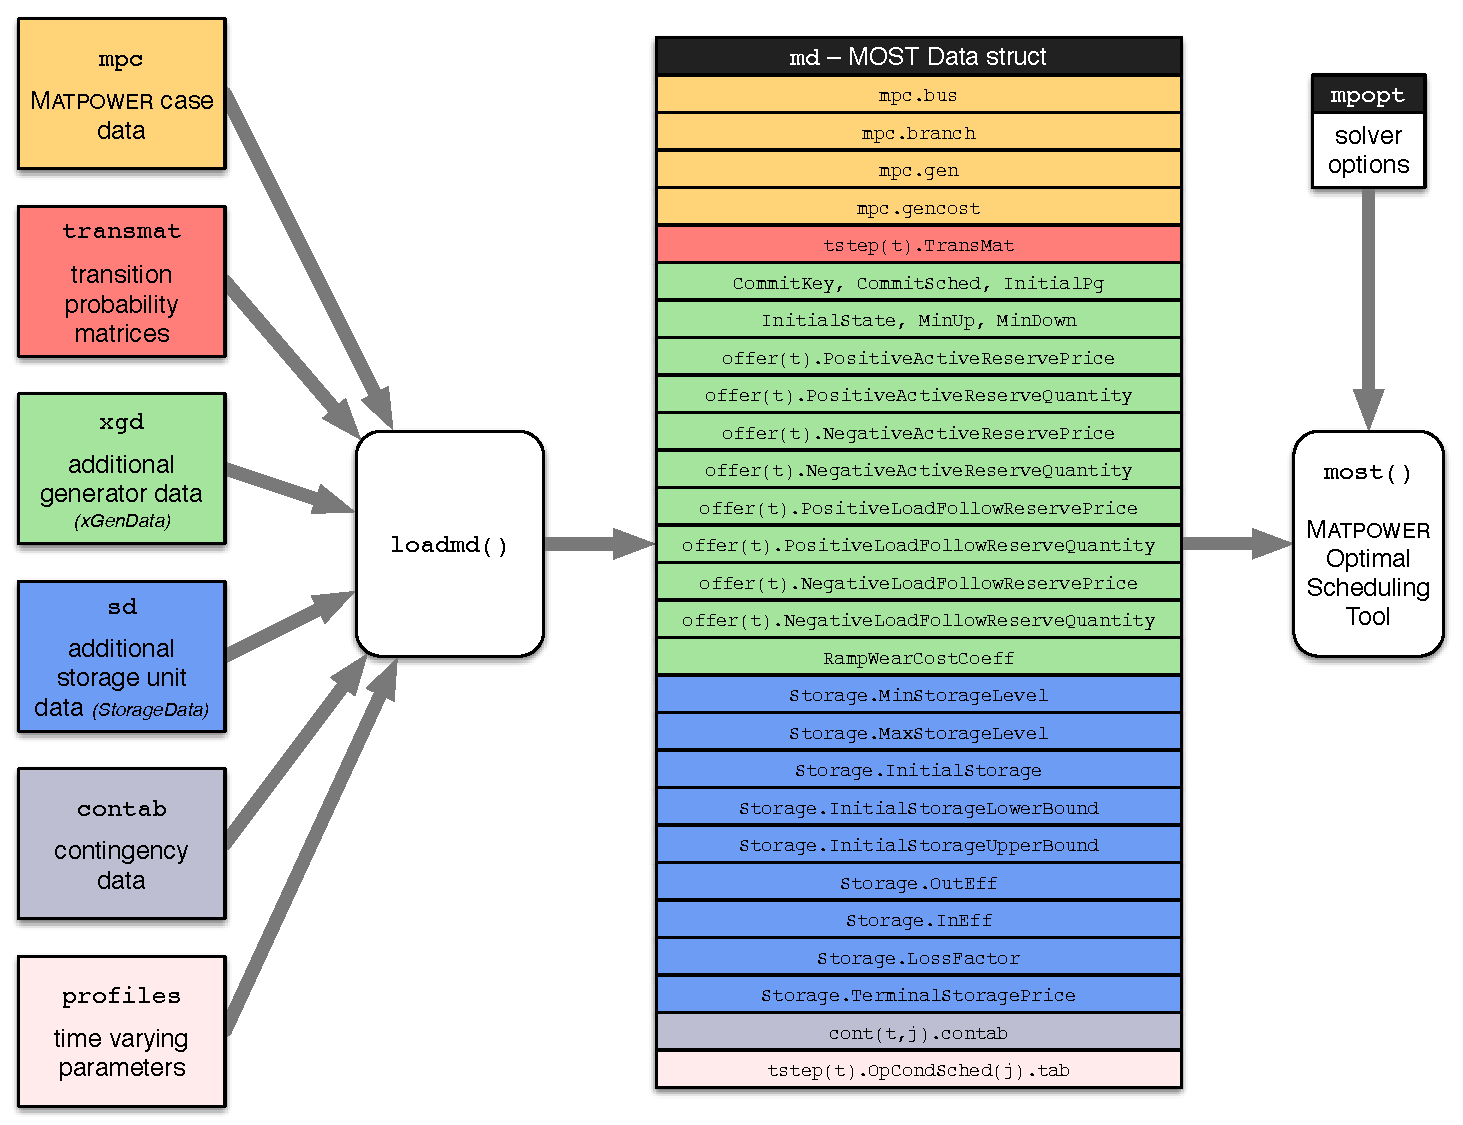
\includegraphics[width=\textwidth]{./figures/loadmd}
  \caption{Assembling the \md{}}
  \label{fig:loadmd}
\end{figure}

The following sections describe the input arguments to \code{loadmd} and the way they are normally constructed.
Except for the transition probability matrices, all parameters which vary from period to period are specified via \code{profiles}, as per-period changes applied to a set of base values provided in the other input arguments.

Since the input arguments to \code{loadmd} are handled by \code{loadgenericdata} (see Section~\ref{sec:loadgenericdata} for details), they can either take the form of the data structure described in each section below, or a string containing the name of an M-file or MAT-file that returns the required data structure.

\subsubsection{{\tt mpc} -- \matpower{} Case}
\label{sec:mpc}

The \mpc{} argument is a \matpower{} case,\footnote{It is important that this case have consecutively numbered buses starting at 1 (i.e. internal ordering). See \matpower{}'s \code{ext2int} function in Section~\ref{MUM-sec:ext2int} of the \mum{} for converting a case to internal ordering.} specified either as a file name or a struct, to be passed by \code{loadmd} as an input to \code{loadcase} from Section~\ref{MUM-sec:loadcase} in the \mum{}.
This case corresponds to the base case from which all other cases, corresponding to different time periods, scenarios and contingency states, are built using change tables and the \code{apply\_changes} function described in Section~\ref{MUM-sec:apply_changes} in the \mum{}.

If the problem you are setting up includes storage resources or wind generators, it may be simpler to exclude these from the \gen{} matrix in \mpc{} and add them later using the \code{addstorage} and \code{addwind} functions described below in Sections~\ref{sec:addstorage} and \ref{sec:addwind}.

\subsubsection{{\tt transmat} -- Transition Probability Matrices}
\label{sec:transmat}

In the general case of a stochastic model with multiple base scenarios per period, \code{transmat} is a cell array of length~$n_t$ containing the transition probability matrices $\Phi^t$ of \eqref{eq:transmat}.
That is, \code{transmat\{t\}} contains the $n_{J^t} \times n_{J^{(t-1)}}$ matrix of transition probabilities from period~$t-1$ to period~$t$.
The first element \code{transmat\{1\}} is a column vector of transition probabilities from period~0 ($n_{J^t} = 1$) to period~1.

For deterministic models or secure models with contingencies but only a single base scenario per period, \code{transmat} can simply be an integer $n_t$ specifying the number of periods in the planning horizon and it will be expanded internally to a cell array of 1's with the appropriate length.
If the problem is also single period, \code{transmat} is optional, with a default value of~1.

\subsubsection{{\tt xgd} -- Extra Generator Data ({\tt xGenData})}
\label{sec:xgd}

The optional \code{xgd} argument is an \code{xGenData} struct containing base values for all of the per-generator data required for the problem that are not included in \mpc{}, that is, in the standard \matpower{} case data.
This includes unit commitment (UC) data, reserve offer data, ramping costs, and more.
Table~\ref{tab:xgd} presents the details of the \code{xGenData} struct, whose fields are all $n_g \times 1$ vectors of per generator values.

An \code{xGenData} struct is typically created from a data file or struct in the \code{xGenDataTable} format via the \code{loadxgendata} function described in Section~\ref{sec:loadxgendata}.
In this context, all fields are optional and \code{loadxgendata} will provide defaults for anything not explicitly specified. The \code{addstorage} and \code{addwind} functions described in Sections~\ref{sec:addstorage} and \ref{sec:addwind} also return \code{xGenData} by calling the \code{loadxgendata} function internally.

\begin{table}[!ht]
%\renewcommand{\arraystretch}{1.2}
\centering
\begin{threeparttable}
\caption{Fields\tnote{*} of \code{xGenData} struct (\code{xgd})}
\label{tab:xgd}
\footnotesize
\begin{tabular}{lcp{0.43\textwidth}}
\toprule
name & default\tnote{\dag} & description \\
\midrule
\code{CommitSched}	&	\code{C} &  0 or 1, UC status to use for non-UC runs	\\
\code{InitialPg}	&	\code{P} &  active power dispatch at time~$t=0$	\\
\code{TerminalPg}	&	&  active power dispatch at time~$t=n_t+1$ \emph{(only included if explicitly specified)}	\\
\code{RampWearCostCoeff}	&	0 &  quadratic coefficient for $C_\delta^i(\cdot)$\tnote{\ddag}~ in \eqref{eq:rampcost} 	\\
\code{PositiveActiveReservePrice}	&	0 & linear coefficient for $C_{R+}^{ti}(\cdot)$\tnote{\ddag}~ in \eqref{eq:most_cres_cost} 	\\
\code{PositiveActiveReserveQuantity}	&	\code{R} & max upward reserve quantity $R_{{\rm max}+}^{ti}$ in \eqref{eq:maxresp}	\\
\code{NegativeActiveReservePrice}	&	0 & linear coefficient for $C_{R-}^{ti}(\cdot)$\tnote{\ddag}~ in \eqref{eq:most_cres_cost}	\\
\code{NegativeActiveReserveQuantity}	&	\code{R} & max downward reserve quantity $R_{{\rm max}-}^{ti}$ in \eqref{eq:maxresm}	\\
\code{PositiveActiveDeltaPrice}	&	0 & linear coefficient for $C_{P+}^{ti}(\cdot)$\tnote{\ddag}~ in \eqref{eq:most_energy_cost}	\\
\code{NegativeActiveDeltaPrice}	&	0 & linear coefficient for $C_{P-}^{ti}(\cdot)$\tnote{\ddag}~ in \eqref{eq:most_energy_cost}	\\
\code{PositiveLoadFollowReservePrice}	&	0 & linear coefficient for $C_{\delta+}^{ti}(\cdot)$\tnote{\ddag}~ in \eqref{eq:most_rampres_cost}	\\
\code{PositiveLoadFollowReserveQuantity}	&	\code{R} & max upward ramp reserve $\delta^{ti}_{\rm max+}$ in \eqref{eq:deltapbounds}	\\
\code{NegativeLoadFollowReservePrice}	&	0 & linear coefficient for $C_{\delta-}^{ti}(\cdot)$\tnote{\ddag}~ in \eqref{eq:most_rampres_cost}	\\
\code{NegativeLoadFollowReserveQuantity}	&	\code{R} & max downward ramp reserve $\delta^{ti}_{\rm max-}$ in \eqref{eq:deltambounds}	\\
\code{CommitKey}	&	&  required for problems with UC	\\
&& \begin{tabular}{r @{ -- } p{0.35\textwidth}}
-1 & offline, unit forced \emph{off} \\
0 or 1 & available for UC decisions \\
2 & must run, unit forced \emph{on} \\
\end{tabular}	\\
\code{InitialState}\tnote{\S}	&	$\pm\infty$\tnote{\P}&  if positive (negative), number of uptime (downtime) periods at time $t = 0$	\\
\code{MinUp}\tnote{\S}	&	1 &  minimum up time in number of periods	\\
\code{MinDown}\tnote{\S}	&	1 &  minimum down time in number of periods	\\
\bottomrule
\end{tabular}
\begin{tablenotes}
 \scriptsize
 \item [*] {All fields are $n_g \times 1$ vectors of per-generator values.}
 \item [\dag] {These are defaults provided by \code{loadxgendata}. If \code{gen} is provided, either directly or as the \code{gen} field of \mpc{}, then \code{P = gen(:, PG)}, \code{C = gen(:, GEN\_STATUS)} and \code{R = 2*(gen(:, PMAX) - MIN(0, gen(:, PMIN)))}, otherwise $\code{C}~=~1$, $\code{R}~=~0$ and no default is provided for \code{P} (corresponding field is not optional).}
 \item [\ddag] {Each of these costs $C(\cdot)$ is presented in the formulation as a general function, but is implmented as a simple linear function of the form $C(x) = a x$, where the linear coefficient being supplied is $a$. The only exception is the ramping cost, which has the quadratic form $C_\delta^i(x) = a x^2$.}
 \item [\S] {Requires that \code{CommitKey} be present and non-empty.}
 \item [\P] {Sign is based on \code{C}\tnote{\dag}, i.e. $+\infty$ for \code{C} = 1, $-\infty$ for \code{C} = 0.}
\end{tablenotes}
\end{threeparttable}
\end{table}

\clearpage
\subsubsection{{\tt sd} -- Storage Data ({\tt StorageData})}
\label{sec:sd}

The optional \code{sd} argument is a \code{StorageData} struct containing base values for all of the storage unit data required for the problem that are not included in the standard \matpower{} case \mpc{} or in the \code{xGenData}.

This includes bounds on stored energy (capacities), efficiencies, loss factors, initial and terminal values, prices used to value leftover storage, and more. Table~\ref{tab:sd} presents the details of the \code{StorageData} struct, whose fields are all $n_s \times 1$ vectors of per storage unit values, except where indicated otherwise.

A \code{StorageData} struct is typically created from data files or structs in \code{StorageDataTable} format via the \code{loadstoragedata} function described in Section~\ref{sec:loadstoragedata}. The \code{addstorage} function from Section~\ref{sec:addstorage} also returns \code{StorageData} by calling the \code{loadstoragedata} function internally.

\begin{table}[!ht]
%\renewcommand{\arraystretch}{1.2}
\centering
\begin{threeparttable}
\caption{Fields\tnote{*} of \code{StorageData} struct (\code{sd})}
\label{tab:sd}
\footnotesize
\begin{tabular}{lcp{0.52\textwidth}}
\toprule
name & default & description \\
\midrule
\code{UnitIdx}	&	\emph{none} &  corresponding row index into \gen{} matrix	\\
\code{ExpectedTerminalStorageAim}	& \emph{none}\tnote{\dag}	 &  target value for expected final stored energy at end of last period, overrides any values provided for both \code{ExpectedTerminalStorageMin} and \code{ExpectedTerminalStorageMax}	\\
\code{ExpectedTerminalStorageMax}	& \emph{none}\tnote{\dag}	 &  upper bound $S_{\rm max}^{n_ti}$ on expected final stored energy at end of last period in \eqref{eq:sftarget}	\\
\code{ExpectedTerminalStorageMin}	& \emph{none}\tnote{\dag}	 &  lower bound $S_{\rm min}^{n_ti}$ on expected final stored energy at end of last period in \eqref{eq:sftarget}	\\
\code{InitialStorage}	&	\emph{none} &  value for initial (expected) stored energy $s_0$	\\
\code{InitialStorageCost}	&	\emph{none}\tnote{\ddag} &  cost $C_{s0}$ associated with starting with amount $s_0$ at time~$t=0$	\\
\code{InitialStorageLowerBound}	&	\emph{none}\tnote{\ddag} &  lower bound $S_{\rm min}^{0i}$ on inital (expected) stored energy $s_0$ in \eqref{eq:s0bounds}	\\
\code{InitialStorageUpperBound}	&	\emph{none}\tnote{\ddag} &  upper bound $S_{\rm max}^{0i}$ on inital (expected) stored energy $s_0$ in \eqref{eq:s0bounds}	\\
\code{InEff}\tnote{\P}	&	1 & input efficiency $\eta^{ti}_{\rm in}$	\\
\code{OutEff}\tnote{\P}	&	1 & output efficiency $\eta^{ti}_{\rm out}$	\\
\code{LossFactor}\tnote{\P}	&	0 & fraction of stored energy lost per hour $\eta^{ti}_{\rm loss}$	\\
\code{MaxStorageLevel}\tnote{\P}	&	\emph{none} & stored energy maximum limit $S^{ti}_{\rm max}$	\\
\code{MinStorageLevel}\tnote{\P}	&	\emph{none} & stored energy minimum limit $S^{ti}_{\rm min}$	\\
\code{rho}\tnote{\P}	&	1 &  $\rho^{ti}$ parameter controlling weighting of worst case ($\rho^{ti} = 1$) and expected values ($\rho^{ti} = 0$) for defining storage constraints in \eqref{eq:storage1st}--\eqref{eq:storagecontingencylast}	\\
\code{TerminalStoragePrice}	&	 &  prices $C_s$ for contributions to terminal storage from charging/discharging in non-terminal states	\\
\code{TerminalChargingPrice0}	&	$C_s$\tnote{\S} &  prices $C_{\rm sc0}$ for contributions to terminal storage from charging in terminal end-of-horizon base states	\\
\code{TerminalDischargingPrice0}	&	$C_s$\tnote{\S} & prices $C_{\rm sd0}$  for contributions to terminal storage from discharging in terminal end-of-horizon base states	\\
\code{TerminalChargingPriceK}	&	$C_s$\tnote{\S} & prices $C_{{\rm sc}k}$ for contributions to terminal storage from charging in terminal contingency states	\\
\code{TerminalDischargingPriceK}	&	$C_s$\tnote{\S} & prices $C_{{\rm sd}k}$ for contributions to terminal storage from discharging in terminal contingency states	\\
\bottomrule
\end{tabular}
\begin{tablenotes}
 \scriptsize
 \item [*] {All fields are $n_s \times 1$ vectors of per storage unit values, except where indicated otherwise. If no default is specified, it means the field is required.}
 \item [\dag] {If the \code{most.storage.terminal\_target} option is set to 0, the \code{ExpectedTerminalStorage*} parameters are optional and ignored; if set to 1, at least one of them is required; if set to $-1$, the presence of any of the optional \code{ExpectedTerminalStorage*} parameters will turn the \code{most.storage.terminal\_target} option on.}
 \item [\ddag] {If the \code{most.storage.cyclic} option is set to 1, \code{InitialStorageCost} is required and the default values of the initial storage bounds \code{InitialStorageLowerBound} and \code{InitialStorageUpperBound} are taken from \code{MinStorageLevel(:, 1)} and \code{MaxStorageLevel(:, 1)}, respectively, otherwise \code{InitialStorageCost} is optional and both initial storage bounds default to \code{InitialStorage}.}
 \item [\P] {Can also be a scalar, in which case the value will be used for all storage units.}
 \item [\S] {That is, the default is taken from \code{TerminalStoragePrice}.}
 \end{tablenotes}
\end{threeparttable}
\end{table}

\subsubsection{{\tt contab} -- Contingency Table}
\label{sec:contab}

The optional \code{contab} argument is a contingency table with a master set of contingencies used for security throughout entire horizon. It is a matrix in the form of a \emph{change table} recognized by \code{apply\_changes}, described in Section~\ref{MUM-sec:apply_changes} in the \mum{}. The probabilities defined in this contingency table correspond to the conditional probabilities $\psi_0^{tjk}$ of contingency~$k$ occuring conditioned on being in base scenario~$j$. While the \md{} (\code{md}) itself allows for contingencies to be defined independently for all scenarios and time periods, \code{loadmd} applies a single set of contingencies and conditional probabilities (single \code{contab}) to all.

\clearpage

\subsubsection{{\tt profiles} -- Profiles for Time-Varying Parameters}
\label{sec:profiles}

Profiles are used to specify how parameters vary from period to period and are defined in terms of changes to a base value. There are currently three different types of data that can be changed by a profile, corresponding to the base values provided by the \mpc{}, \code{xgd} and \code{sd} arguments to \code{loadmd}.

A profile is a struct that specifies, for a given set of changes to be applied across time periods and scenarios, the type of data, the table or field, the elements in that table or field, the method of modification and the values to be applied. Table~\ref{tab:profile} summarizes the structure of the \code{profile} struct.

\begin{table}[!ht]
%\renewcommand{\arraystretch}{1.2}
\centering
\begin{threeparttable}
\caption{Fields of Profle Struct (\code{profile})}
\label{tab:profile}
\footnotesize
\begin{tabular}{lp{0.85\textwidth}}
\toprule
name & description \\
\midrule
\code{type}	&	string defining type of target data structure modified by the profile \\
& \begin{tabular}{l @{ -- } p{0.65\textwidth}}
\codeq{mpcData} & parameters in fields of \mpc{}, e.g. \bus{}, \gen{}, \gencost{}, etc.\tnote{*}  \\
\codeq{xGenData} & parameters in fields of \code{xGenData}, e.g. reserve offers, commitment parameters, etc. \\
\codeq{StorageData} & parameters in fields of \code{StorageData}, e.g. storage capacities, efficiencies, etc. \\
\end{tabular}	\\
\code{table}	&	numeric scalar or string identifying the table or field; valid values depend on \code{type} \\
& \begin{tabular}{l @{ -- } p{0.55\textwidth}}
\code{type} = \codeq{mpcData} &  numeric values defined in Table~\ref{MUM-tab:cttable} in the \mum{} \\
\code{type} = \codeq{xGenData} & string-valued field names defined in Table~\ref{tab:xgd} \\
\code{type} = \codeq{StorageData} & string-valued field names defined in Table~\ref{tab:sd} \\
\end{tabular}	\\
\code{rows}	&	vector of indices of rows (first dimension) of array to be modified, or area indices for area-wide modifications; 0 means ``apply to all'' \\
\code{col}	&	column index or other ID of parameter to modify as defined in Table~\ref{MUM-tab:ctcol} in the \mum{}; ignored unless \code{type} = \codeq{mpcData} \\
\code{chgtype}	&	method of modification, see Table~\ref{MUM-tab:ctchgtype} in the \mum{} \\
\code{values}	&	$n_1 \times n_2 \times n_3$ numeric array containing the new values or scale/shift factors \\
& \begin{tabular}{l @{ -- } p{0.55\textwidth}}
$n_1$ &  corresponds to number of time periods $n_t$ \\
$n_2$ & corresponds to number of scenarios $n_j^{\rm max}$ \\
$n_3$ & corresponds to number of elements indicated by \code{rows} \\
\end{tabular}	\\
& A singleton dimension in \code{values} not matching with $n_t = 1$ or $n_j^{\rm max} = 1$ or \code{length(profile.rows)} = 1 is interpreted as ``apply to all'' whenever the parameter being modified allows such an expansion. \\
\bottomrule
\end{tabular}
\begin{tablenotes}
 \scriptsize
 \item [*] {Possible modifications are as implemented by \matpower{}'s \code{apply\_changes} function. See Section~\ref{MUM-sec:apply_changes} in the \mum{}.}
 \end{tablenotes}
\end{threeparttable}
\end{table}

Section~\ref{sec:idx_profile} describes \code{idx\_profile} which defines a number of constants that are useful for specifying profiles. The \code{apply\_profile} function from Section~\ref{sec:apply_profile} is used internally by \code{loadmd} to apply the profiles. And \code{getprofiles} from Section~\ref{sec:getprofiles} is used to load a profile or set of profiles from a struct, MAT-file or M-file function.


% \subsubsection{{\tt trajdata} -- Trajectory Data}
% \label{sec:trajdata}

\clearpage
\subsection{\most{} Options}
\label{sec:mostoptions}

In addition to making use of the \code{verbose} option and the solver-specific options, such as those under the fields \code{cplex}, \code{glpk}, \code{gurobi}, etc. as documented in Appendix~\ref{MUM-app:options} in the \mum{}, there are also a number of options specific to \most{} that appear under a \code{most} field in the standard \matpower{} options struct. These can be classified into two main categories and are described in Tables~\ref{tab:mostrunoptions} and \ref{tab:mostmodeloptions}. The first consists of options related to how \code{most} is run, such as the solver to use and the phases of the problem building and solving to be included. The second is all of the options controlling various details of the model to be built and solved.

\begin{table}[!ht]
%\renewcommand{\arraystretch}{1.2}
\centering
\begin{threeparttable}
\caption{\most{} Run Options}
\label{tab:mostrunoptions}
\footnotesize
\begin{tabular}{lcp{0.55\textwidth}}
\toprule
name & default & description \\
\midrule
\code{most.solver}	& \codeq{DEFAULT}	& solver option passed in \code{opt.alg} to \code{miqps\_matpower} or \code{qps\_matpower}, see \code{miqps\_matpower} or \code{qps\_matpower} for details	\\
\code{most.skip\_prices}	& 0	& skip price computation stage for mixed integer problems, see \code{miqps\_matpower} for details	\\
\code{most.price\_stage\_warn\_tol}	& $10^{-7}$	& tolerance on the objective function value and primal variable relative match required to avoid mis-match warning message, see \code{miqps\_matpower} for details	\\
\code{most.build\_model}	&  1	& toggle building of MIQP model \\
&& \begin{tabular}{r @{ -- } p{0.5\textwidth}}
0 & do \emph{not} build MIQP, assume it has already been built \\
1 & build MIQP, both constraints and standard costs (not coordination cost\tnote{\dag}~) and store in \code{mdo.QP} \\
\end{tabular}	\\
\code{most.solve\_model}	& 1	& toggle solving of MIQP model	\\
&& \begin{tabular}{r @{ -- } p{0.5\textwidth}}
0 & do \emph{not} solve MIQP, assume it is just being built; requires \codeq{most.build\_model} set to 1 \\
1 & solve MIQP; if coordination cost\tnote{\dag}~ exists, update it; requires either \codeq{most.build\_model} set to 1 or \code{mdi.QP} must contain previously built model \\
\end{tabular}	\\
\code{most.resolve\_new\_cost}	& 0	& toggle solving pre-built MIQP with updated coordination cost\tnote{\ddag}	\\
&& \begin{tabular}{r @{ -- } p{0.5\textwidth}}
0 & build full MIQP from scratch, then solve \\
1 & solve pre-built MIQP with updated coordination cost\tnote{\dag} \\
\end{tabular}	\\
\bottomrule
\end{tabular}
\begin{tablenotes}
 \scriptsize
 \item [\dag] {Coordination costs are related to a price coordination scheme employed in a decomposition used for solving the non-linear AC formulation \emph{(not yet implemented)}.}
 \item [\ddag] {Requires \codeq{most.solve\_model} set to 1.}
\end{tablenotes}
\end{threeparttable}
\end{table}


\begin{table}[!ht]
%\renewcommand{\arraystretch}{1.2}
\centering
\begin{threeparttable}
\caption{\most{} Model Options}
\label{tab:mostmodeloptions}
\footnotesize
\begin{tabular}{lcp{0.5\textwidth}}
\toprule
name & default & description \\
\midrule
\code{most.dc\_model}	& 1	& power balance model	\\
&& \begin{tabular}{r @{ -- } p{0.43\textwidth}}
0 & use simple total power balance constraint
$\sum {\rm generation} = \sum {\rm demand}$ \\
1 & use DC power flow network model \\
\end{tabular}	\\
\code{most.q\_coordination}	& 0	& create $q^{tijk}$ variables for reactive power coordination (0 or 1)	\\
\code{most.fixed\_res}	& $-1$	& include fixed zonal reserve constraints \eqref{eq:most_zres_cost}, \eqref{eq:reserve_var2}--\eqref{eq:reserve_req2} for security	\\
&& \begin{tabular}{r @{ -- } p{0.43\textwidth}}
$-1$ & if fixed zonal reserves specified \\
0 & never \\
1 & always \\
\end{tabular}	\\
\code{most.security\_constraints}	& $-1$	& include contingency constraints for security	\\
&& \begin{tabular}{r @{ -- } p{0.43\textwidth}}
$-1$ & if contingencies specified \\
0 & never \\
1 & always \\
\end{tabular}	\\
\code{most.storage.terminal\_target}	& $-1$	& constrain expected terminal storage to a target range\tnote{\dag}	\\
&& \begin{tabular}{r @{ -- } p{0.43\textwidth}}
$-1$ & if target range specified \\
0 & never \\
1 & always \\
\end{tabular}	\\
\code{most.storage.cyclic}	& 0	& use cyclic storage constraints \eqref{eq:sfequals0}\tnote{\dag}	\\
&& \begin{tabular}{r @{ -- } p{0.43\textwidth}}
0 & \emph{off}, initial storage $s_0^i$ is a fixed parameter, no constraint on final expected storage $s_F^{n_ti}$\\
1 & \emph{on}, initial storage $s_0^i$ is an optimization variable constrained to equal final expected storage $s_F^{n_ti}$ \\
\end{tabular}	\\
\code{most.uc.run}	& $-1$	& flag to indicate whether to perform unit commitment	\\
&& \begin{tabular}{r @{ -- } p{0.43\textwidth}}
-1 & perform unit commitment if and only if \code{mdi.UC.CommitKey} is present and non-empty \\
0 & do \emph{not} perform unit commitment \\
1 & \emph{do} perform unit commitment \\
\end{tabular}	\\
\code{most.uc.cyclic}	& 0	& commitment restrictions (e.g. min up and down times) roll over from end of horizon back to beginning (0 or 1)	\\
\code{most.alpha}	& 0	& $\alpha$, for contingency states, fraction of period spent in base state before contingency occurs (0--1)	\\
\bottomrule
\end{tabular}
\begin{tablenotes}
 \scriptsize
 \item [\dag] {The \code{most.storage.terminal\_target} and \code{most.storage.cyclic} options cannot be used simultaneously (i.e. at least one of them must be set to 0).}
\end{tablenotes}
\end{threeparttable}
\end{table}

\clearpage
\subsection{\md{}}
\label{sec:md}

\subsubsection{Input Data}
\label{sec:mdinputdata}

The input to the \code{most} function takes the form of a \md{}, a single \matlab{} struct \code{md}, with the primary input fields described in Tables~\ref{tab:md_inputs} through \ref{tab:md_inputstorage}. As described previously in Section~\ref{sec:inputdata}, a \md{} is typically not constructed directly, but rather assembled from various other inputs by the \code{loadmd} function. However, some of the features, such as fixed zonal reserve requirements, binary transition masks for load-following ramp, or linear dynamical system constraints, are only available by modifying portions of the \md{} directly.

\begin{table}[!ht]
%\renewcommand{\arraystretch}{1.2}
\centering
\begin{threeparttable}
\caption{Input Data Fields of \code{md}}
\label{tab:md_inputs}
\footnotesize
\begin{tabular}{lccp{0.5\textwidth}}
\toprule
name & type\tnote{*} & default & description \\
\midrule
\code{cont(t,j).contab}	& I	 & \emph{empty}	 & changes table\tnote{\dag}~ defining contingencies for period~$t$, scenario~$j$ \\
\code{Delta\_T}	& I	 & 1	 & length of time step in hours \\
\code{idx.nt}	& I	 & 	 & number of periods in scheduling horizon \\
\code{InitialPg(i)}	& I	 & 	 & $n_g \times 1$, injection of generator~$i$ at $t = 0$ \\
\code{mpc}	& I	 & 	 & base system data, standard \matpower{} case struct\tnote{\ddag}, with \baseMVA{}, \bus{}, \gen{}, \branch{} and \gencost{} fields \\
\code{offer(t)}	& I	 & 	 & struct with offer data for period~$t$, see Table~\ref{tab:md_inputoffer} for details of sub-fields \\
\code{OpenEnded}	& I	 & 1	 & ignore terminal dispatch ramp constraints, \emph{deprecated} \\
\code{RampWearCostCoeff(i,t)}	& I	 & 0	 & $n_g \times n_t$, cost of ramping of generator~$i$ from period~$t-1$ to $t$, coefficient $C_\delta^i$ for square of dispatch difference in \eqref{eq:rampcost} \\
\code{Storage}	& B	 & 	 & struct with parameters for storage units, see Table~\ref{tab:md_inputstorage} for the input fields \\
\code{TerminalPg(i)}	& I	 & 	 & $n_g \times 1$, injection of generator~$i$ at $t = n_t$, \emph{deprecated, untested} \\
\code{tstep(t)}	& B	 & 	 &  $n_t \times 1$ struct of parameters related to period~$t$ \\
\code{~~~.OpCondSched(j).tab}	& I	 & 	 & changes table defining modifications from \mpc{} for each base scenario~$j$ in period~$t$	\\
\code{~~~.TransMask}	& I	 & 	 & an $n_{j(t)} \times n_{j(t-1)}$ matrix of binary transition masks $\zeta^{tj_2j_1}$ from scenario~$j_1$ in period~$t-1$ to $j_2$ in period $t$, see Section~\ref{sec:filter_ramp_transitions}	\\
\code{~~~.TransMat}	& I	 & 	 & $\Phi^t$, an $n_{j(t)} \times n_{j(t-1)}$ matrix of transition probabilities $\phi^{tj_2j_1}$ from scenario~$j_1$ in period~$t-1$ to $j_2$ in period $t$, see Section~\ref{sec:transmat}	\\
\bottomrule
\end{tabular}
\begin{tablenotes}
 \scriptsize
 \item [*] {I = input, O = output, B = both, opt = taken from \matpower{} options.}
 \item [\dag] {See Section~\ref{sec:contab} for details. Note that, while \code{loadmd} assigns the same \code{contab} to all $t$ and $j$, it is possible to set different \code{contab} values manually and they will be respected by \code{most}.}
 \item [\ddag] {See Appendix~\ref{MUM-app:caseformat} in the \mum{} for details.}
\end{tablenotes}
\end{threeparttable}
\end{table}

\begin{table}[!ht]
%\renewcommand{\arraystretch}{1.2}
\centering
\begin{threeparttable}
\caption{Additional Input Data Fields of \code{md}}
\label{tab:md_inputs2}
\footnotesize
\begin{tabular}{lccp{0.5\textwidth}}
\toprule
name & type\tnote{*} & default & description \\
\midrule
\code{CoordCost}	& I	 & \emph{empty}	 & user supplied coordination costs for AC version \\
\code{~~~.Huser}	& I	 & 	 & sparse matrix of quadratic coefficients \\
\code{~~~.Cuser}	& I	 & 	 & vector of linear coefficients \\
\code{~~~.cuser}	& I	 & 	 & scalar constant term \\
\code{dstep(t)}	& I	 & \emph{empty}	 & $n_t^{\rm ds} \times 1$ struct with parameters for optional dynamical system model, \eqref{eq:dynbounds}--\eqref{eq:dynout2}  \\
\code{~~~.A}	& I	 & 	 & $A_{\rm ds}^t$, from \eqref{eq:dynstate1}--\eqref{eq:dynstate2} \\
\code{~~~.B}	& I	 & 	 & $B_{\rm ds}^t$, from \eqref{eq:dynstate1} \\
\code{~~~.C}	& I	 & 	 & $C_{\rm ds}^t$, from \eqref{eq:dynout1}--\eqref{eq:dynout2} \\
\code{~~~.D}	& I	 & 	 & $D_{\rm ds}^t$, from \eqref{eq:dynout1} \\
\code{~~~.ymin}	& I	 & 	 & $y_{\rm min}^t$, lower bound on output from \eqref{eq:dynout1}--\eqref{eq:dynout2} \\
\code{~~~.ymax}	& I	 & 	 & $y_{\rm max}^t$, upper bound on output from \eqref{eq:dynout1}--\eqref{eq:dynout2} \\
\code{~~~.zmin}	& I	 & 	 & $z_{\rm min}^t$, lower bound on $z^t$ from \eqref{eq:dynbounds} \\
\code{~~~.zmax}	& I	 & 	 & $z_{\rm max}^t$, upper bound on $z^t$ from \eqref{eq:dynbounds} \\
\code{FixedReserves(t,j,k)}	& I	 & \emph{empty}	 & zonal reserve input parameters for  period~$t$, scenario~$j$, contingency~$k$, in form of \code{reserves} field of \mpc{} from Table~\ref{MUM-tab:reserves} in the \mum{}, with \code{cost}, \code{qty}, \code{zones}, \code{req} sub-fields. \\
\code{UC}	& B	 & 	 & struct with unit commitment parameters \\
\code{~~~.CommitKey(i,t)}	& I	 & \emph{empty}	 & optional $n_g \times n_t$ vector specifying availability of unit~$i$ for commitment at time~$t$ \\
&&& \begin{tabular}{r @{ -- } p{0.35\textwidth}}
-1 & offline, unit forced \emph{off} \\
0 or 1 & available for UC decisions \\
2 & must run, unit forced \emph{on} \\
\end{tabular}	\\
\code{~~~.CommitSched(i,t)}	& B	 & 	 & $n_g \times n_t$ matrix UC status (0 or 1) of unit~$i$ at time~$t$, input for non-UC runs, result for UC runs \\
\code{~~~.InitialState(i)}\tnote{\dag}	& I	 & \emph{empty}	 & $n_g \times 1$ vector of initial states,
if positive (negative), number of uptime (downtime) periods at time t = 0 \\
\code{~~~.MinUp(i)}\tnote{\dag}	& I	 & \emph{empty}	 & $n_g \times 1$ vector, minimum up time in number of periods \\
\code{~~~.MinDown(i)}\tnote{\dag}	& I	 & \emph{empty}	 & $n_g \times 1$ vector, minimum down time in number of periods \\
\code{z1}	& I	 & \emph{empty}	 & initial state $z^1$ of optional dynamical system model \\
\bottomrule
\end{tabular}
\begin{tablenotes}
 \scriptsize
 \item [*] {I = input, O = output, B = both, opt = taken from \matpower{} options.}
 \item [\dag] {Requires that \code{CommitKey} be present and non-empty.}
\end{tablenotes}
\end{threeparttable}
\end{table}


\begin{table}[!ht]
%\renewcommand{\arraystretch}{1.2}
\centering
\begin{threeparttable}
\caption{Fields of Offer struct \code{md.offer(t)}}
\label{tab:md_inputoffer}
\footnotesize
\begin{tabular}{lp{0.55\textwidth}}
\toprule
name & description \\
\midrule
\code{PositiveActiveReservePrice}\tnote{\dag}	& linear coefficient of $C_{RP+}^{ti}(\cdot)$ in \eqref{eq:mostobjective} 	\\
\code{PositiveActiveReserveQuantity}\tnote{\dag}	& max upward reserve quantity $R_{P{\rm max}+}^{ti}$ in \eqref{eq:maxresp}	\\
\code{NegativeActiveReservePrice}\tnote{\dag}	& linear coefficient of $C_{RP-}^{ti}(\cdot)$ in \eqref{eq:mostobjective}	\\
\code{NegativeActiveReserveQuantity}\tnote{\dag}	& max downward reserve quantity $R_{P{\rm max}-}^{ti}$ in \eqref{eq:maxresm}	\\
\code{PositiveActiveDeltaPrice}\tnote{\dag}	& linear coefficient of $C_{P+}^{ti}(\cdot)$ in \eqref{eq:mostobjective}	\\
\code{NegativeActiveDeltaPrice}\tnote{\dag}	& linear coefficient of $C_{P-}^{ti}(\cdot)$ in \eqref{eq:mostobjective}	\\
\code{PositiveLoadFollowReservePrice}\tnote{\dag}	& linear coefficient of $C_{\delta+}^{ti}(\cdot)$ in \eqref{eq:mostobjective}	\\
\code{PositiveLoadFollowReserveQuantity}\tnote{\dag}	& max upward ramp reserve $\delta^{ti}_{\rm max+}$ in \eqref{eq:deltapbounds}	\\
\code{NegativeLoadFollowReservePrice}\tnote{\dag}	& linear coefficient of $C_{\delta-}^{ti}(\cdot)$ in \eqref{eq:mostobjective}	\\
\code{NegativeLoadFollowReserveQuantity}\tnote{\dag}	& max downward ramp reserve $\delta^{ti}_{\rm max-}$ in \eqref{eq:deltambounds}	\\
\code{gencost}\tnote{\ddag}	& energy offers in the form of generator cost functions	\\
\bottomrule
\end{tabular}
\begin{tablenotes}
 \scriptsize
 \item [\dag] {$n_g \times 1$ vector of values for each generator at time~$t$.}
 \item [\ddag] {Deprecated. Use profiles instead.}
\end{tablenotes}
\end{threeparttable}
\end{table}


\begin{table}[!ht]
%\renewcommand{\arraystretch}{1.2}
\centering
\begin{threeparttable}
\caption{Input Fields of \code{md.Storage}}
\label{tab:md_inputstorage}
\footnotesize
\begin{tabular}{lccp{0.43\textwidth}}
\toprule
name & type\tnote{*} & default & description\tnote{\dag} \\
\midrule
\code{UnitIdx(i)}	& I 	& 	& corresponding \gen{} matrix row index	\\
\code{ExpectedTerminalStorageAim(i)}	& I 	& 	& target value for expected final stored energy at end of last period for storage unit~$i$, overrides any values provided for both \code{ExpectedTerminalStorageMin} and \code{ExpectedTerminalStorageMax} 	\\
\code{ExpectedTerminalStorageMax(i)}	& I 	& 	& upper bound $S_{\rm min}^{n_ti}$ on expected final stored energy in \eqref{eq:sftarget} 	\\
\code{ExpectedTerminalStorageMin(i)}	& I 	& 	& lower bound $S_{\rm max}^{n_ti}$ on expected final stored energy in \eqref{eq:sftarget} 	\\
\code{InitialStorage(i)}	& B 	& 	& initial (expected) stored energy $s_0$ in MWh	\\
\code{InitialStorageCost(i)}	& I 	& 	& cost $C_{s0}$ associated with starting with amount $s_0$ at time~$t=0$ 	\\
\code{InitialStorageLowerBound(i)}	& I 	& 	& lower bound $S_{\rm min}^{0i}$ on inital (expected) stored energy $s_0$ in \eqref{eq:s0bounds} 	\\
\code{InitialStorageUpperBound(i)}	& I 	& 	& upper bound $S_{\rm max}^{0i}$ on inital (expected) stored energy $s_0$ in \eqref{eq:s0bounds} 	\\
\code{InEff(i,t)}\tnote{\ddag}	& I 	& 1	& input efficiency $\eta^{ti}_{\rm in}$ 	\\
\code{OutEff(i,t)}\tnote{\ddag}	& I 	& 1	& output efficiency $\eta^{ti}_{\rm out}$ 	\\
\code{LossFactor(i,t)}\tnote{\ddag}	& I 	& 0	& fraction of stored energy lost per hour $\eta^{ti}_{\rm loss}$	\\
\code{MaxStorageLevel(i,t)}\tnote{\ddag}	& I 	& 	& stored energy maximum limit $S^{ti}_{\rm max}$ 	\\
\code{MinStorageLevel(i,t)}\tnote{\ddag}	& I 	& 	& stored energy minimum limit $S^{ti}_{\rm min}$ 	\\
\code{rho(i,t)}	& I 	& 	& $\rho^{ti}$ parameter controlling weighting of worst case ($\rho^{ti} = 1$) and expected values ($\rho^{ti} = 0$) for defining storage constraints in \eqref{eq:storage1st}--\eqref{eq:storagecontingencylast}	\\
\code{TerminalStoragePrice(i)}	& I 	& 	& prices $C_s$ for contributions to terminal storage from charging/discharging in non-terminal states	\\
\code{TerminalChargingPrice0(i)}	& I 	& $C_s$\tnote{\S}	& prices $C_{\rm sc0}$ for \dots charging in terminal end-of-horizon base states	\\
\code{TerminalChargingPriceK(i)}	& I 	& $C_s$\tnote{\S}	& prices $C_{{\rm sc}k}$ for \dots charging in terminal contingency states	\\
\code{TerminalDischargingPrice0(i)}	& I 	& $C_s$\tnote{\S}	& prices $C_{\rm sd0}$  for \dots discharging in terminal end-of-horizon base states	\\
\code{TerminalDischargingPriceK(i)}	& I 	& $C_s$\tnote{\S}	& prices $C_{{\rm sd}k}$ for \dots discharging in terminal contingency states	\\
\bottomrule
\end{tabular}
\begin{tablenotes}
 \scriptsize
 \item [*] {I = input, O = output, B = both, opt = taken from \matpower{} options.}
 \item [\dag] {All fields have $n_s$ rows, where row~$i$ refers to storage unit~$i$. See also Table~\ref{tab:sd}.}
 \item [\ddag] {Automatically expanded from scalar, $n_s \times 1$ or $1 \times n_t$ vector to a full $n_s \times n_t$ matrix.}
 \item [\S] {That is, the default is taken from \code{TerminalStoragePrice}.}
\end{tablenotes}
\end{threeparttable}
\end{table}

\clearpage
\subsubsection{Output Data}
\label{sec:mdoutputdata}

Additional fields are initialized or added to the \md{} by \code{most} and returned in the updated output struct. Some simply record the values of corresponding options found in the \matpower{} options struct passed in, while others contain computed results. The output fields added or updated by \code{most} are summarized in Tables~\ref{tab:md_outputs} through \ref{tab:md_results}.

\begin{table}[!ht]
%\renewcommand{\arraystretch}{1.2}
\centering
\begin{threeparttable}
\caption{Output Data Fields of \code{md}}
\label{tab:md_outputs}
\footnotesize
\begin{tabular}{lcp{0.5\textwidth}}
\toprule
name & type\tnote{*} & description \\
\midrule
\code{alpha}	& opt	 & $\alpha$, copy of  \code{most.alpha} option \\
\code{CostWeights(k,j,t)}\tnote{\dag}	& O	 & $\psi^{tjk}$, probability of contingency~$k$ in scenario~$j$ at time~$t$ \\
\code{CostWeightsAdj(k,j,t)}\tnote{\dag}	& O	 & $\psi_\alpha^{tjk}$, same as $\psi^{tjk}$, but adjusted for $\alpha$ as in \eqref{eq:psialpha} \\
\code{DCMODEL}	& opt	 & copy of \code{most.dc\_model} option \\
\code{flow(t,j,k)}	& O	 & case data for period~$t$, scenario~$j$, contingency~$k$ \\
\code{~~~.mpc}	&	& \matpower{} case struct,\tnote{\ddag}~ prices and gen costs are probability-weighted	\\
\code{~~~.PLsh}	&	& vector needed to compute branch flow results \\
\code{idx}	& B	 & various problem dimensions, see Table~\ref{tab:md_inputidx}	\\
\code{IncludeFixedReserves}	& opt	 & copy of \code{most.fixed\_res} option \\
\code{QCoordination}	& opt	 & copy of \code{most.q\_coordination} option \\
\code{QP}	& B\tnote{\P}	 & (MI)QP/LP problem setup and results, see Table~\ref{tab:md_qp} \\
\code{results}	& O	 & results, see Table~\ref{tab:md_results} \\
\code{SecurityConstrained}	& opt	 & copy of \code{most.security\_constraints} option \\
\code{StepProb(t)}	& O	 & $\gamma^t$, probability of making it to period~$t$ \\
\code{Storage}	& B	 & $\gamma^t$, probability of making it to period~$t$ \\
\code{~~~.ExpectedStorageDispatch(i,t)}	& O 	& $n_s \times n_t$, expected dispatch of storage unit~$i$	\\
\code{~~~.ExpectedStorageState(i,t)}	& O 	& $n_s \times n_t$, expected stored energy in storage unit~$i$ at end period~$t$	\\
\code{~~~.ForceCyclicStorage}	& opt 	& copy of \code{most.storage.cyclic} option	\\
\code{~~~.ForceExpectedTerminalStorage}	& opt 	& copy of \code{most.storage.terminal\_target} option	\\
\code{~~~.InitialStorage(i)}	& B 	& $n_s \times 1$, initial (expected) stored energy $s_0$ in MWh, computed as output when \code{most.storage.cyclic} option is on	\\
\code{tstep(t)}	& B	 & $n_t \times 1$ struct of parameters related to period~$t$ \\
\code{~~~.E}\tnote{\S}	& O	 & $E^t$, used to compute expected injections in period~$t$	\\
\code{~~~.G}\tnote{\S}	& O	 & $G^t$	\\
\code{~~~.H}\tnote{\S}	& O	 & $H^t$	\\
\code{~~~.Li}\tnote{\S}	& O	 & $L_I^t$	\\
\code{~~~.Lf}\tnote{\S}	& O	 & $L_F^t$	\\
\code{~~~.Mg}\tnote{\S}	& O	 & $M^t_g$	\\
\code{~~~.Mh}\tnote{\S}	& O	 & $M^t_h$	\\
\code{~~~.Ng}\tnote{\S}	& O	 & $N^t_g$	\\
\code{~~~.Nh}\tnote{\S}	& O	 & $N^t_h$	\\
\code{UC.CommitSched(i,t)}	& B	 & $n_g \times n_t$ matrix UC status (0 or 1) of unit~$i$ at time~$t$, input for non-UC runs, result for UC runs \\
\bottomrule
\end{tabular}
\begin{tablenotes}
 \scriptsize
 \item [*] {I = input, O = output, B = both, opt = taken from \matpower{} options.}
 \item [\dag] Note index order -- \code{(:,:,t)} refers to period~$t$.
 \item [\ddag] {See Appendix~\ref{MUM-app:caseformat} in the \mum{} for details.}
 \item [\P] {The \code{QP} field is either contructed by \code{most} or taken as an input, based on the value of the \code{most.build\_model} option described in Table~\ref{tab:mostrunoptions}.}
 \item [\S] {Used to compute expected inital and final storage amounts for period~$t$. See \eqref{eq:simnall}--\eqref{eq:Nth} for details.}
\end{tablenotes}
\end{threeparttable}
\end{table}

\begin{table}[!ht]
%\renewcommand{\arraystretch}{1.2}
\centering
\begin{threeparttable}
\caption{Fields of Index struct \code{md.idx}}
\label{tab:md_inputidx}
\footnotesize
\begin{tabular}{lcp{0.7\textwidth}}
\toprule
name & type\tnote{*} & description \\
\midrule
\code{nt}	& I	 & number of periods in scheduling horizon \\
\code{nj(t)}	& O	 & number of base scenarios for period~$t$, computed from length of \code{tstep(t).OpCondSched(j)}	\\
\code{nc(t,j)}	& O	 & number of contingencies in period~$t$, scenario~$j$	\\
\code{nb(t,j,k)}	& O	 & number of buses in period~$t$, scenario~$j$, contingency~$k$	\\
\code{nb\_total}	& O	 & total number of buses summed over all flows	\\
\code{ng}	& O	 & number of gens in \code{mpc.gen}	\\
\code{ny(t,j,k)}	& O	 & number of gens with piecewise linear costs in period~$t$, scenario~$j$, contingency~$k$	\\
\code{nf\_total}	& O	 & total number of flows (periods~$t$ $\times$ scenarios~$j$ $\times$ contingencies~$k$)	\\
\code{ns}	& O	 & number of storage units	\\
\code{ns\_total}	& O	 &\code{ns} $\times$ \code{nf\_total}	\\
\code{ntramp}	& O	 & number of periods of load-following reserves, always equal to \code{nt - 1} since \code{OpenEnded} has been deprecated	\\
\code{ntds}	& O	 & $n_t^{\rm ds}$, number of time periods in the horizon of the dynamical system model	\\
\code{nzds}	& O	 & $n_z^{\rm ds}$, size of state vector for dynamical system model \eqref{eq:dynstate1}-\eqref{eq:dynstate2}	\\
\code{nyds}	& O	 & $n_y^{\rm ds}$, number of outputs of dynamical system model \eqref{eq:dynout1}-\eqref{eq:dynout2}	\\
\code{nvars}	& O	 & total number of variables	\\
\bottomrule
\end{tabular}
\begin{tablenotes}
 \scriptsize
 \item [*] {I = input, O = output, B = both, opt = taken from \matpower{} options.}
 \item [\dag] {Used to compute expected inital and final storage amounts for period~$t$. See \eqref{eq:simnall}--\eqref{eq:Nth} for details.}
\end{tablenotes}
\end{threeparttable}
\end{table}


\begin{table}[!ht]
%\renewcommand{\arraystretch}{1.2}
\centering
\begin{threeparttable}
\caption{Fields of QP struct \code{md.QP}}
\label{tab:md_qp}
\footnotesize
\begin{tabular}{lcp{0.7\textwidth}}
\toprule
name & type\tnote{*} & description \\
\midrule
\code{A}\tnote{\S}	& B	 & linear constraint matrix	\\
\code{l}\tnote{\S}	& B	 & linear constraint lower bound	\\
\code{u}\tnote{\S}	& B	 & linear constraint upper bound	\\
\code{x}\tnote{\S}	& O	 & full optimization variable $x$	\\
\code{f}\tnote{\S}	& O	 & value of objective function at solution (same as \code{md.results.f})	\\
\code{vtype}\tnote{\S}	& B	 & string containing variable types	\\
\code{x0}\tnote{\S}	& B	 & variable initial value	\\
\code{xmin}\tnote{\S}	& B	 & variable lower bound	\\
\code{xmax}\tnote{\S}	& B	 & variable upper bound	\\
\code{H}\tnote{\S}	& B	 & quadratic cost coefficient matrix\tnote{\dag}	\\
\code{C}\tnote{\S}	& B	 & linear cost coefficient vector\tnote{\dag}	\\
\code{c}	& B	 & constant cost term\tnote{\dag}	\\
\code{H1}	& B	 & quadratic cost coefficient matrix\tnote{\ddag}	\\
\code{C1}	& B	 & linear cost coefficient vector\tnote{\ddag}	\\
\code{c1}	& B	 & constant cost term\tnote{\ddag}	\\
\code{Cfstor}	& B	 & linear cost coefficients of full $x$ to reflect expected value of storage in terminal states	\\
\code{opt}\tnote{\S}	& B	 & options struct for \code{qps\_matpower} or \code{miqps\_matpower}, set by \most{} run options and solver-specific \matpower{} options via \code{mpopt2qpopt}	\\
\code{exitflag}\tnote{\S}	& O	 & 1 = converged successfully, 0 or negative value = solver specific failure code	\\
\code{output}\tnote{\S}	& O	 & struct with solver-specific fields and \code{alg} field specifying solver that was used	\\
\code{lambda}\tnote{\S}	& O	 & Lagrange and Kuhn-Tucker multipliers on constraints \\
\code{~~~.mu\_l}\tnote{\S}	& O	 & lower (left-hand) limit on linear constraints \\
\code{~~~.mu\_u}\tnote{\S}	& O	 & upper (right-hand) limit on linear constraints \\
\code{~~~.lower}\tnote{\S}	& O	 & lower bound on optimization variables \\
\code{~~~.upper}\tnote{\S}	& O	 & upper bound on optimization variables \\
\bottomrule
\end{tabular}
\begin{tablenotes}
 \scriptsize
 \item [*] {I = input, O = output, B = both, opt = taken from \matpower{} options. The \code{QP} struct and its fields are either contructed by \code{most} or taken as an input, based on the value of the \code{most.build\_model} option described in Table~\ref{tab:mostrunoptions}.}
 \item [\dag] {Including user defined coordination costs from \code{md.CoordCost}.}
 \item [\ddag] {Excluding user defined coordination costs from \code{md.CoordCost}.}
 \item [\S] {See input and output arguments for \code{qps\_matpower} or \code{miqps\_matpower} for details.}
\end{tablenotes}
\end{threeparttable}
\end{table}


\begin{table}[!ht]
%\renewcommand{\arraystretch}{1.2}
\centering
\begin{threeparttable}
\caption{Fields of Results struct \code{md.results}}
\label{tab:md_results}
\footnotesize
\begin{tabular}{lcp{0.7\textwidth}}
\toprule
name & type\tnote{*} & description \\
\midrule
\code{f}	& O	& value of objective function $f(x)$ in \eqref{eq:mostobjective} at solution (same as \code{md.QP.f})	\\
\code{success}	& O	& optimization success flag, 1 = succeeded, 0 = failed	\\
\code{Pc(i,t)}	& O	& $n_g \times n_t$, active power contract quantity, $p_c^{ti}$	\\
\code{Rpp(i,t)}	& O	& $n_g \times n_t$, upward active contingency reserve quantity $r_+^{ti}$	\\
\code{Rpm(i,t)}	& O	& $n_g \times n_t$, downward active contingency reserve quantity $r_-^{ti}$	\\
\code{Rrp(i,t)}	& O	& $n_g \times n_t$, upward load-following ramping reserve quantity $\delta_+^{ti}$	\\
\code{Rrm(i,t)}	& O	& $n_g \times n_t$, downward load-following ramping reserve quantity $\delta_-^{ti}$	\\
\code{Sp}	& O	& $n_s \times n_t$, endogenously computed upper stored energy bounds $s_+^{ti}$	\\
\code{Sm}	& O	& $n_s \times n_t$, endogenously computed lower stored energy bounds $s_-^{ti}$	\\
\code{GenPrices(i,t)}	& O	& $n_g \times n_t$, expected energy price	\\
\code{CondGenPrices(i,t)}	& O	& $n_g \times n_t$, expected energy price, conditional on making it to time~$t$	\\
\code{RppPrices(i,t)}	& O	& $n_g \times n_t$, price on upward active contingency reserve	\\
\code{RpmPrices(i,t)}	& O	& $n_g \times n_t$, price on downward active contingency reserve	\\
\code{RrpPrices(i,t)}	& O	& $n_g \times n_t$, price on upward load-following ramping reserve	\\
\code{RrmPrices(i,t)}	& O	& $n_g \times n_t$, price on downward load-following ramping reserve	\\
\code{ExpectedRampCost(i,t)}	& O	& $n_g \times n_t$, expected ramping cost (wear and tear)	\\
\code{ExpectedDispatch(i,t)}	& O	& $n_g \times n_t$, expected generator dispatch across base cases	\\
\code{Z}	& O	& $n_z^{\rm ds} \times n_t^{\rm ds}$, dynamical system model state $z$	\\
\code{Y}	& O	& $n_y^{\rm ds} \times n_t^{\rm ds}$, dynamical system model output	\\
\code{SetupTime}	& O	& time to construct model in seconds	\\
\code{SolveTime}	& O	& time to solve model in seconds	\\
\bottomrule
\end{tabular}
\begin{tablenotes}
 \scriptsize
 \item [*] {I = input, O = output, B = both, opt = taken from \matpower{} options.}
\end{tablenotes}
\end{threeparttable}
\end{table}

\clearpage
\subsection{Additional Considerations}
\label{sec:mostmisc}

The current version of \most{} has a number of modeling limitations relative to \matpower{}. The following is a list of \matpower{} features that are not yet supported by \most{}:
\begin{itemize}
\item branch angle difference limits
\item branch flow soft limits
\item DC transmission lines
\item full non-linear AC network modeling
\item interface flow limits
\end{itemize}

%%------------------------------------------
\clearpage
\section{Additional Functions}

\subsection{\tt addgen2mpc}
\label{sec:addgen2mpc}

\begin{Code}
  [new_mpc, idx] = addgen2mpc(mpc, gen, gencost, gen_type)
\end{Code}

Appends a set of generators to those contained in an existing \matpower{} case struct.
The existing case in \mpc{} is a standard \matpower{} case with additional fields, \code{genfuel} containing a cell array of string-valued fuel types (one for each generator), and \code{i<type>} containing (for each fuel type) a vector of indices of the generators of type \code{<type>}.
The \gen{} and \gencost{} inputs are the standard \matpower{} generator and generator cost matrices and \code{gen\_type} is a string or cell array of strings of fuel types for the generators to be appended.

It returns the updated case struct in \code{new\_mpc}, with the new generators appended to the \gen{}, \gencost{} and \code{genfuel} fields and updated \code{i<type>} fields, along with a vector \code{idx} of indices of the newly added generators.

While there are no canonical definitions for generator types, Table~\ref{tab:gen_types} contains some strings that have been used by convention, where \codeq{ess} and \codeq{wind} are used explicitly by some functions in \most{}.

\begin{table}[!ht]
%\renewcommand{\arraystretch}{1.2}
\centering
\begin{threeparttable}
\caption{Typical Generator Types}
\label{tab:gen_types}
\footnotesize
\begin{tabular}{ll}
\toprule
type string & description \\
\midrule
\codeq{biomass}	&	biomass	\\
\codeq{coal}	&	coal	\\
\codeq{dl}	&	dispatchable load	\\
\codeq{ess}	&	energy storage system	\\
\codeq{hydro}	&	hydro	\\
\codeq{ng}	&	natural gas, combustion turbine	\\
\codeq{ngcc}	&	natural gas, combined cycle	\\
\codeq{nuclear}	&	nuclear	\\
\codeq{oil}	&	oil	\\
\codeq{refuse}	&	refuse	\\
\codeq{solar}	&	solar PV	\\
\codeq{syncgen}	&	synchronous condensor	\\
\codeq{wind}	&	wind	\\
\codeq{na}	&	\emph{none}	\\
\codeq{unknown}	&	\emph{unknown}	\\
\bottomrule
\end{tabular}
\end{threeparttable}
\end{table}


\subsection{\tt addstorage}
\label{sec:addstorage}

\begin{Code}
  [idx, new_mpc] = addstorage(storage, mpc)
  [idx, new_mpc, new_xgd, new_sd] = addstorage(storage, mpc)
  [idx, new_mpc, new_xgd, new_sd] = addstorage(storage, mpc, xgd)
  [idx, new_mpc, new_xgd, new_sd] = addstorage(storage, mpc, xgd, sd)
\end{Code}

Given a \code{StorageUnitData} struct (\code{storage}), or the name of a function or MAT-file containing such a struct, this function adds the specified storage units, modeled as additional special generators, to the existing \gen{} and \gencost{} matrices of the \matpower{} case (\mpc{}) and to the existing \code{xGen} and \code{StorageData} structs, providing a convenient way to specify in one place all of the parameters for a set of storage units.

The parameters for the storage units to be added are specified in a \code{StorageUnitData} struct, which is a single struct with the four fields described in Table~\ref{tab:storage_unit_data}.
Return values include a vector \code{idx} of generator indices for the newly added storage units, along with updated versions of the \mpc{}, \code{xgd} and \code{sd} structs specified by the inputs..

\begin{table}[!ht]
%\renewcommand{\arraystretch}{1.2}
\centering
\begin{threeparttable}
\caption{Fields of \code{StorageUnitData} struct (\code{storage})}
\label{tab:storage_unit_data}
\footnotesize
\begin{tabular}{lcp{0.65\textwidth}}
\toprule
name & default & description \\
\midrule
\gen{}	&	\emph{none} &	rows to be appended to the \gen{} matrix\tnote{*}~ in \mpc{} \\
\gencost{}	&	\emph{zero cost} &	rows to be appended to the \gencost{} matrix\tnote{*}~ in \mpc{} \\
\code{xgd\_table}	&	\emph{none} &	\code{xGenDataTable} struct\tnote{\dag}~ corresponding to units to be added \\
\code{sd\_table}	&	\emph{none} &	\code{StorageDataTable} struct\tnote{\ddag}~ corresponding to units to be added \\
\bottomrule
\end{tabular}
\begin{tablenotes}
 \scriptsize
 \item [*] {See Tables~\ref{MUM-tab:gendata} and \ref{MUM-tab:gencostdata} in Appendix~\ref{MUM-app:caseformat} of the \mum{} for details on the format.}
 \item [\dag] {See \code{loadxgendata} in Section~\ref{sec:loadxgendata} and Table~\ref{tab:xgd_table} for details of the \code{xGenDataTable} struct.}
 \item [\ddag] {See \code{loadstoragedata} in Section~\ref{sec:loadstoragedata} and Table~\ref{tab:sd_table} for details of the \code{StorageDataTable} struct.}
 \end{tablenotes}
\end{threeparttable}
\end{table}


\subsection{\tt addwind}
\label{sec:addwind}

\begin{Code}
  [idx, new_mpc] = addwind(wind, mpc)
  [idx, new_mpc, new_xgd] = addwind(wind, mpc)
  [idx, new_mpc, new_xgd] = addwind(wind, mpc, xgd)
\end{Code}

Given a \code{WindUnitData} struct (\code{wind}), or the name of a function or MAT-file containing such a struct, this function adds the specified wind generators to the existing \gen{} and \gencost{} matrices of the \matpower{} case (\mpc{}) and to the existing \code{xGen} struct, providing a convenient way to specify in one place all of the parameters for a set of wind generators.

The parameters for the wind generators to be added are specified in a \code{WindUnitData} struct, which is a single struct with the four fields described in Table~\ref{tab:wind_unit_data}.
Return values include a vector \code{idx} of generator indices for the newly added wind generators, along with updated versions of the \mpc{} and \code{xgd} structs specified by the inputs.

\begin{table}[!ht]
%\renewcommand{\arraystretch}{1.2}
\centering
\begin{threeparttable}
\caption{Fields of \code{WindUnitData} struct (\code{wind})}
\label{tab:wind_unit_data}
\footnotesize
\begin{tabular}{lcp{0.65\textwidth}}
\toprule
name & default & description \\
\midrule
\gen{}	&	\emph{none} &	rows to be appended to the \gen{} matrix\tnote{*}~ in \mpc{} \\
\gencost{}	&	\emph{zero cost} &	rows to be appended to the \gencost{} matrix\tnote{*}~ in \mpc{} \\
\code{xgd\_table}	&	\emph{none} &	\code{xGenDataTable} struct\tnote{\dag}~ corresponding to units to be added \\
\bottomrule
\end{tabular}
\begin{tablenotes}
 \scriptsize
 \item [*] {See Tables~\ref{MUM-tab:gendata} and \ref{MUM-tab:gencostdata} in Appendix~\ref{MUM-app:caseformat} of the \mum{} for details on the format.}
 \item [\dag] {See \code{loadxgendata} in Section~\ref{sec:loadxgendata} and Table~\ref{tab:xgd_table} for details of the \code{xGenDataTable} struct.}
 \end{tablenotes}
\end{threeparttable}
\end{table}

\subsection{\tt apply\_profile}
\label{sec:apply_profile}

\begin{Code}
  chgtabs = apply_profile( profile, chgtabsi )
  xgd     = apply_profile( profile, xgdi, dim )
  sd      = apply_profile( profile, sdi, dim )
\end{Code}

The \code{apply\_profile} function applies a single profile of a given type to the provided input. See Section~\ref{sec:profiles} and Table~\ref{tab:profile} for details on the profile struct.

For profiles of type \codeq{mpcData}, the output is an $n_t \times n_j^{\rm max}$ cell array of \emph{change tables} in the format expected by \matpower{}'s \code{apply\_changes} function.\footnote{See Section~\ref{MUM-sec:apply_changes} in the \mum{}.} The second input is also $n_t \times n_j^{\rm max}$ cell array. Each element can be either empty or contain a change table to which the new changes are appended.

For profiles of type \codeq{xGenData} the second argument is the \code{xGenData}  struct to be modified (\code{xgdi}) and the output \code{xgd} is a modified version of the same struct.
The the third argument \code{dim} is a positive integer indicating the number of elements corresponding to the third dimension of \code{profile.values}. This allows this dimension to be expanded to the appropriate size if it is specified as a singleton dimension in \code{profile.values}.

Profiles of type \codeq{StorageData} are completely analogous, taking a \code{StorageData} struct (\code{sdi}) as the second input and returning a modified version of it in \code{sd}.

\subsection{\tt filter\_ramp\_transitions}
\label{sec:filter_ramp_transitions}

\begin{Code}
  md = filter_ramp_transitions(md0, threshold)
\end{Code}

The \code{filter\_ramp\_transitions} function creates a binary valued transition mask $\zeta^{tj_2j_1}$ for ramping reserves based on a given probability \code{threshold}. Only transitions with probabilities greater than or equal to a given \code{threshold} value are included, where the probability of the transition from state~$j_1$ to $j_2$ is taken to be the conditional probability $\Phi^t$ from \eqref{eq:transmat}, specified in the \code{transmat} argument to \code{loadmd}, multiplied by the conditional probability of being in state~$j_1$, given that you've made it to period~$t$.

\subsection{\tt getprofiles}
\label{sec:getprofiles}

\begin{Code}
  profiles = getprofiles(profilesi);
  profiles = getprofiles(profilesi, profiles0);
  profiles = getprofiles(profilesi, idx);
  profiles = getprofiles(profilesi, profiles0, idx);
\end{Code}

Loads a profile or set of profiles from a struct, MAT-file or M-file (\code{profilei}),
optionally using the $n$-dimensional index vector \code{idx} to modify any non-zero values in the \code{rows} fields so that the corresponding \code{rows} field in the returned \code{profiles} is equal to \code{idx(rows)}.
This makes it easy to use profiles defined for a particular set of generators, such as those added to a case as a group by \code{addwind} or \code{addstorage}.

The optional \code{profiles0} argument allows the user to provide an existing profile struct to which the new profiles are appended.

\subsection{\tt idx\_profile}
\label{sec:idx_profile}

\begin{Code}
  [PR_REP, PR_REL, PR_ADD, PR_TCONT, PR_TYPES, PR_TMPCD,...
      PR_TXGD, PR_TCTD, PR_TSTGD, PR_CHGTYPES] = idx_profile;
\end{Code}

This function defines constants that are useful in defining profiles.

\begin{table}[!ht]
%\renewcommand{\arraystretch}{1.2}
\centering
\begin{threeparttable}
\caption{Constants Defined by \code{idx\_profile}}
\label{tab:idx_profile}
\footnotesize
\begin{tabular}{lcl}
\toprule
name & value & description \\
\midrule
\code{PR\_REP}	& 1 	& replace old values with new ones \\
\code{PR\_REL}	& 2 	& multiply old values by scale factors \\
\code{PR\_ADD}	& 3 	& add shift factor to old values \\
\code{PR\_TCONT}\tnote{*}	& 1 	&  \\
\code{PR\_TYPES}	& \emph{list} 	& list of profile types \\
\code{PR\_TMPCD}	& \emph{list} 	& vector of valid table types for \codeq{mpcData} \\
\code{PR\_TXGD}	& \emph{list} 	& list of valid table types for \codeq{xGenData} \\
\code{PR\_TCTD}\tnote{*}	& \emph{list} 	& list of valid table types for \codeq{ContingencyData} \\
\code{PR\_TSTGD}	& \emph{list} 	& list of valid table types for \codeq{StorageData} \\
\code{PR\_CHGTYPES}	& \emph{list} 	& list of valid change types \\
\bottomrule
\end{tabular}
\begin{tablenotes}
 \scriptsize
 \item [*] {Related to functionality not yet implemented.}
 \end{tablenotes}
\end{threeparttable}
\end{table}


\subsection{\tt loadgenericdata}
\label{sec:loadgenericdata}

\begin{Code}
  var = loadgenericdata(varfile, vartype)
  var = loadgenericdata(varfile, vartype, fields)
  var = loadgenericdata(varfile, vartype, fields, varname)
  var = loadgenericdata(varfile, vartype, fields, varname, args)
\end{Code}

The \code{loadgenericdata} function loads data from a variable, M-file or MAT-file and checks that it matches a specified type.
The first argument, \code{varfile}, is a variable containing the data structure or a string containing the name of a function M-file or a MAT-file on the \matlab{} path.
If no file extension is provided, it will attempt to load a MAT-file with the specified name and, if not found, will call a function by that name to get the data.
The function M-file should return a single argument containing the data.
A MAT-file should either contain a single variable with the desired data or provide the variable name in \code{varname}.

The second argument, \code{vartype}, is a string or cell array of strings with, in order of priority, the data structure type to be returned.
Valid values are \codeq{struct}, \codeq{cell} and \codeq{array}.

The third argument, \code{fields}, is optional and contains a string or cell array of strings containing a list of required fields in case the \code{vartype} is \codeq{struct}.
If a required field is missing it will throw an error.

The \code{varname} and \code{args} arguments are also optional.
\code{varname} is a string containing the name of the variable to extract when loading a MAT-file.
If not provided, the default is to extract the first variable, regardless of name.
And \code{args} is a scalar or cell array of values that are passed as input arguments to the function, in the case where \code{varfile} is a function name.

\subsection{\tt loadmd}
\label{sec:loadmd}

\begin{Code}
  md = loadmd(mpc, transmat, xgd, sd, contab, profiles)
\end{Code}

The \code{loadmd} function provides the canonical way of loading a \md{}. For details please see Sections~\ref{sec:mpc}--\ref{sec:profiles}.

\subsection{\tt loadstoragedata}
\label{sec:loadstoragedata}

\begin{Code}
  sd = loadstoragedata(sd_table)
  sd = loadstoragedata(sd_table, gen)
  sd = loadstoragedata(sd_table, mpc)
\end{Code}

The \code{loadstoragedata} function provides the canonical way of loading additional parameters for storage resources into a \code{StorageData} struct, described in Section~\ref{sec:sd} and summarized in Table~\ref{tab:sd}.
It takes a \code{StorageDataTable} struct as input,
either directly or as the name of a function or MAT-file that returns such a struct.
If the optional second argument is provided, either a \matpower{} \gen{} matrix or a \matpower{} case file \mpc{}, the number of storage units is checked for consistency.

The \code{StorageDataTable} struct is used as a convenient way to define the \code{StorageData} struct using a table format for the data and is summarized in Table~\ref{tab:sd_table}.
It has two mandatory fields, \code{colnames} and \code{data}.
The \code{data} field is a $n_s \times N$ matrix, where $n_s$ is the number of storage units and $N$ is the number of fields in the \code{StorageData} being defined.
The \code{colnames} field is an $N$ dimensional cell array of strings with field names corresponding to the columns in \code{data}.
The number of columns in the table and their order are determined by the user, depending on the fields for which they want to specify non-default values.

\begin{table}[!ht]
%\renewcommand{\arraystretch}{1.2}
\centering
\begin{threeparttable}
\caption{Fields of \code{StorageDataTable} struct (\code{sd\_table})}
\label{tab:sd_table}
\footnotesize
\begin{tabular}{lcp{0.65\textwidth}}
\toprule
name & default & description \\
\midrule
\code{colnames}	&	\emph{none} &  $N$ element cell array of \code{StorageData} field names\tnote{*}~ corresponding to the columns of the \code{data} field\tnote{\dag}	\\
\code{data}	&	\emph{none} & $n_s \times N$ matrix of storage parameters\tnote{\dag}	\\
\code{MinStorageLevel}\tnote{\ddag}	&	\emph{none} & stored energy minimum limit $S^{ti}_{\rm min}$	\\
\code{MaxStorageLevel}\tnote{\ddag}	&	\emph{none} & stored energy maximum limit $S^{ti}_{\rm max}$	\\
\code{OutEff}\tnote{\ddag}	&	1 & output efficiency $\eta^{ti}_{\rm out}$	\\
\code{InEff}\tnote{\ddag}	&	1 & input efficiency $\eta^{ti}_{\rm in}$	\\
\code{LossFactor}\tnote{\ddag}	&	0 & fraction of stored energy lost per hour $\eta^{ti}_{\rm loss}$	\\
\code{rho}\tnote{\ddag}	&	1 &  $\rho^{ti}$ parameter controlling weighting of worst case ($\rho^{ti} = 1$) and expected values ($\rho^{ti} = 0$) for defining storage constraints in \eqref{eq:storage1st}--\eqref{eq:storagecontingencylast}	\\
\bottomrule
\end{tabular}
\begin{tablenotes}
 \scriptsize
 \item [*] {See Table~\ref{tab:sd} for a list of valid field names.}
 \item [\dag] {$n_s$ is the number of storage units and $N$ is the number of fields in the \code{StorageData} being defined by the given \code{StorageDataTable}.}
 \item [\ddag] {Values in these scalar fields are overridden by any corresponding values in the \code{data} table.}
 \end{tablenotes}
\end{threeparttable}
\end{table}

There are six additional optional scalar fields that can be used instead of the \code{data} table if a single value is to be assigned uniformly to all of the storage units. An example \code{StorageDataTable} struct is created by the following code.

\begin{Code}
storage.sd_table.OutEff     = 0.9;
storage.sd_table.InEff      = 0.9;
storage.sd_table.LossFactor = 0.02;
storage.sd_table.rho        = 0;
storage.sd_table.colnames = {  % indented to align with data cols
    'InitialStorage', ...
        'InitialStorageLowerBound', ...
            'InitialStorageUpperBound', ...
                'InitialStorageCost', ...
                    'TerminalStoragePrice', ...
                        'MinStorageLevel', ...
                            'MaxStorageLevel', ...
};
storage.sd_table.data = [
    40  0   80  45  43  0   40;
    30  0   60  47  45  0   30;
    50  0   100 46  44  0   50;
];
\end{Code}

See also the \code{addstorage} function in Section~\ref{sec:addstorage} for a potentially more convenient way to specify all of the parameters for your storage resources in a single file or struct.

\subsection{\tt loadxgendata}
\label{sec:loadxgendata}

\begin{Code}
  xgd = loadxgendata(xgd_table)
  xgd = loadxgendata(xgd_table, gen)
  xgd = loadxgendata(xgd_table, mpc)
\end{Code}

The \code{loadxgendata} function provides the canonical way of loading extra generator data into an \code{xGenData} struct
described in Section~\ref{sec:xgd} and summarized Table~\ref{tab:xgd}.
It takes an \code{xGenDataTable} struct as input,
either directly or as the name of a function or MAT-file that returns such a struct.
If the optional second argument is provided, either a \matpower{} \gen{} matrix or a \matpower{} case file \mpc{}, the generator status and limits are used to set certain default values as indicated in Table~\ref{tab:xgd}.

The \code{xGenDataTable} struct is used as a convenient way to define the \code{xGenData} struct using a table format for the data and is summarized in Table~\ref{tab:xgd_table}.
It has two fields, \code{colnames} and \code{data}.
The \code{data} field is a $n_g \times N$ matrix, where $n_g$ is the number of generators and $N$ is the number of fields in the \code{xGenData} being defined.
Those that are not defined in the \code{xGenDataTable} struct are assigned default values by \code{loadxgendata}.
The \code{colnames} field is an $N$ dimensional cell array of strings with field names corresponding to the columns in \code{data}.
The number of columns in the table and their order are determined by the user, depending on the fields for which they want to specify non-default values.

\begin{table}[!ht]
%\renewcommand{\arraystretch}{1.2}
\centering
\begin{threeparttable}
\caption{Fields of \code{xGenDataTable} struct (\code{xgd\_table})}
\label{tab:xgd_table}
\footnotesize
\begin{tabular}{lcp{0.75\textwidth}}
\toprule
name & default & description \\
\midrule
\code{colnames}	&	\emph{none} &  $N$ element cell array of \code{xGenData} field names\tnote{*}~ corresponding to the columns of the \code{data} field\tnote{\dag}	\\
\code{data}	&	\emph{none} & $n_g \times N$ matrix of extra generator parameters\tnote{\dag}	\\
\bottomrule
\end{tabular}
\begin{tablenotes}
 \scriptsize
 \item [*] {See Table~\ref{tab:xgd} for a list of valid field names.}
 \item [\dag] {$n_g$ is the number of generators and $N$ is the number of fields in the \code{xGenData} being defined by the given \code{xGenDataTable}.}
 \end{tablenotes}
\end{threeparttable}
\end{table}

 An example \code{xGenDataTable} struct is created by the following code.
 
\begin{Code}
xgd_table.colnames = {  % indented to align with data cols
    'CommitSched', ...
        'PositiveActiveReservePrice', ...
            'PositiveActiveReserveQuantity' };
xgd_table.data = [
    1   5   25;
    1   8   200;
    1   20  60;
    1   2   100;
];
\end{Code}

\clearpage
\subsection{\tt most\_summary}
\label{sec:most_summary}

\begin{Code}
  most_summary(mdo)
  ms = most_summary(mdo)
\end{Code}

\emph{This function should be considered experimental.
It is included because it is often better than nothing, though it is very incomplete.}

Given a \md{} returned by \code{most}, this function returns a struct with the fields listed in Table~\ref{tab:most_summary}.
Printing to the console is currently controlled by the \code{mdo.QP.verbose} flag.

\begin{table}[!ht]
%\renewcommand{\arraystretch}{1.2}
\centering
\begin{threeparttable}
\caption{Fields of \code{most\_summary} struct (\code{ms})}
\label{tab:most_summary}
\footnotesize
\begin{tabular}{lp{0.75\textwidth}}
\toprule
name & description \\
\midrule
\code{f}	& objective function value	\\
\code{nb}	& $n_b$, number of buses	\\
\code{ng}	& $n_g$, number of generators (incl. storage, disp. load, etc.)	\\
\code{nl}	& $n_l$, number of branches	\\
\code{ns}	& $n_s$, number of storage units	\\
\code{nt}	& $n_t$, number of periods in planning horizon	\\
\code{nj\_max}	& $n_j^{\rm max}$, max number of scenarios per period	\\
\code{nc\_max}	& $n_c^{\rm max}$, max number of contingencies per scenario in any period	\\
\code{psi}	& $n_t \times n_j^{\rm max} \times (n_c^{\rm max}+1)$, adjusted cost weights, $\psi_\alpha^{tjk}$, see \eqref{eq:psialpha}	\\
\code{Pg}	& $n_g \times n_t \times n_j^{\rm max} \times (n_c^{\rm max}+1)$, real power generation	\\
\code{Pd}	& $n_b \times n_t \times n_j^{\rm max} \times (n_c^{\rm max}+1)$, fixed real power demand	\\
\code{Rup}	& $n_g \times n_t$, upward ramping reserve quantities	\\
\code{Rdn}	& $n_g \times n_t$, downward ramping reserve quantities	\\
\code{SoC}	& $n_s \times n_t$, expected stored energy (state-of-charge)	\\
\code{Pf}	& $n_g \times n_t \times n_j^{\rm max} \times (n_c^{\rm max}+1)$, real power generation	\\
\code{u}	& $n_g \times n_t \times n_j^{\rm max} \times (n_c^{\rm max}+1)$, generator commitment status	\\
\code{lamP}	& $n_b \times n_t \times n_j^{\rm max} \times (n_c^{\rm max}+1)$, shadow price on power balance	\\
\code{muF}	& $n_l \times n_t \times n_j^{\rm max} \times (n_c^{\rm max}+1)$, shadow price on flow limits	\\
\bottomrule
\end{tabular}
\end{threeparttable}
\end{table}

\clearpage
\subsection{\tt mostver}
\label{sec:mostver}

\begin{Code}
  mostver
  vnum = mostver
  v = mostver('all')
\end{Code}

Called with no output arguments, \code{mostver} prints the version number and release date of the current \most{} installation. Otherwise, if called with no input arguments, it returns the current version as a string and with any true input argument, such as the string \codeq{all}, it returns a struct with the fields \code{Name}, \code{Version}, \code{Release} and \code{Date} (all strings).


%%------------------------------------------
\clearpage
\section{Tutorial Examples}
\label{sec:tutorial}

The examples in this section are based on the simple three bus model summarized in Table~\ref{tab:threebus} and illustrated in Figure~\ref{fig:threebus}. The case data can be found in the \code{ex\_case3a} and \code{ex\_case3b} files. Not all examples include every part of the model. For example, the single-period deterministic examples do not have the wind generator at bus~2, none of the deterministic cases include the contingencies and the stochastic cases do not include the fixed reserve requirement. The storage unit is only included where specifically mentioned.

\begin{table}[!ht]
%\renewcommand{\arraystretch}{1.2}
\centering
\begin{threeparttable}
\caption{Summary of Tutorial Example System Data}
\label{tab:threebus}
\footnotesize
\begin{tabular}{ll}
\toprule
\bf{topology}	& 3-bus triangle network	\\
\midrule
	& 2 identical 200 MW gens at bus 1, different reserve cost	\\
\bf{generators}	& 500 MW gen at bus 2	\\
	& all 3 have identical quadratic generation costs\tnote{*}	\\
\midrule
\bf{load}	& 450 MW at bus 3	\\
	& curtailable at \$1000/MWh	\\
\midrule
	& 300 MW limit, line 1--2	\\
\bf{branches}	& 240 MW limit, line 1--3	\\
	& 300 MW limit, line 2--3	\\
\midrule
\bf{adequacy requirement}	& option 1: 150 MW system requirement	\\
	& option 2: contingencies: \begin{tabular}{l}
- generator 2 at bus 1 \\
- line 1--3 \\
\end{tabular}	\\
\midrule
\bf{wind}	& unit at bus 2 with 100 MW output in nominal case	\\
	& stochastic cases use 3 samples of normal distribution	\\
\midrule
\bf{storage}	& 200 MWh unit at bus 3	\\
	& 80 MW max charge/discharge rate	\\
\bottomrule
\end{tabular}
\begin{tablenotes}
 \scriptsize
 \item [*] {Linear costs of \$25, \$30, and \$40/WMh are used for some examples.}
\end{tablenotes}
\end{threeparttable}
\end{table}

\begin{figure}[hbt]
  \centering
  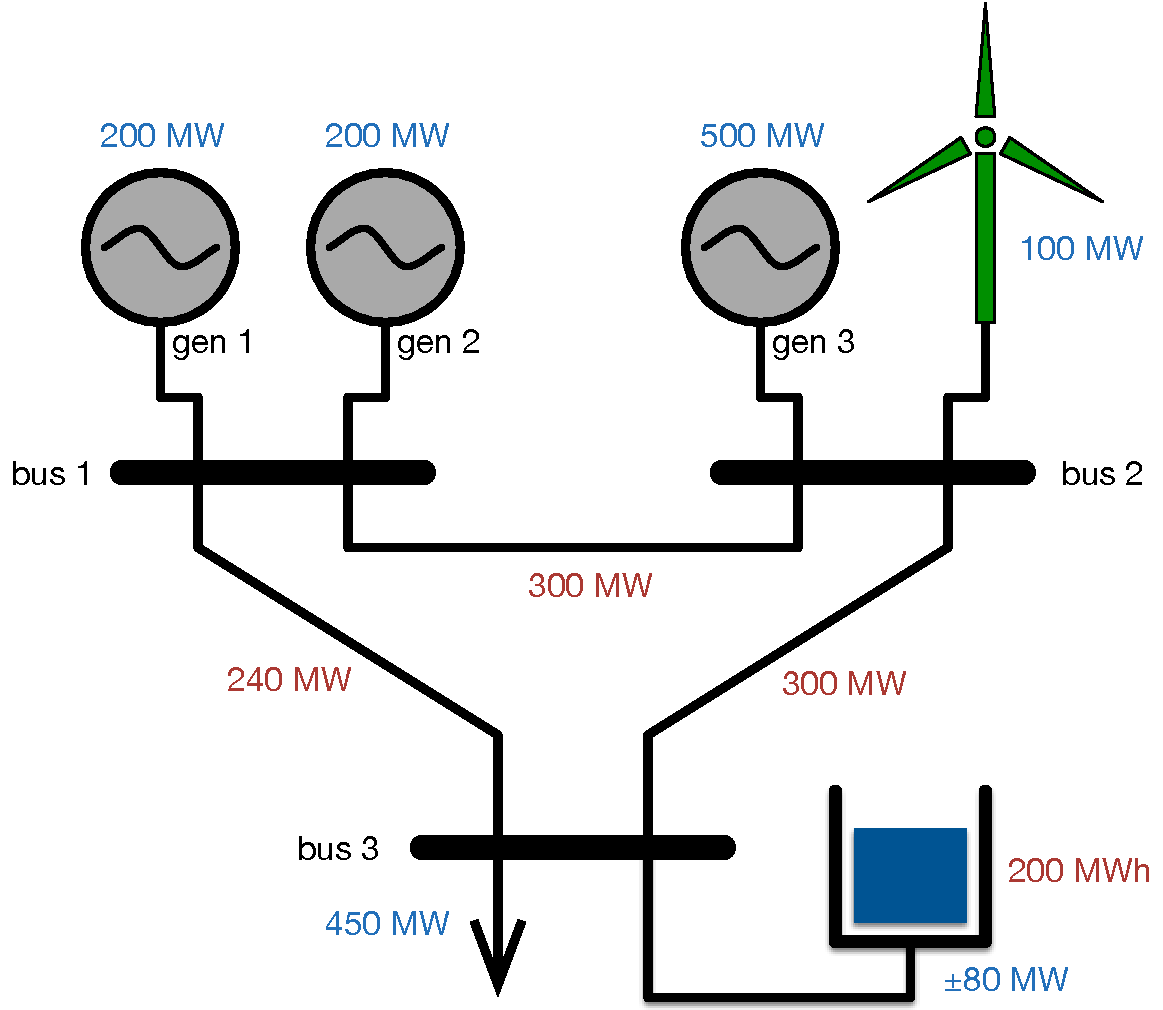
\includegraphics[width=0.75\textwidth]{./figures/3-bus-ex}
  \caption{Tutorial Example System}
  \label{fig:threebus}
\end{figure}

The code for the following examples can be found in \mostpath{/lib/t} in the files whose names begin with \code{most\_ex}, such as \code{most\_ex1\_ed.m}.
For all of the following examples, assume that \code{mpopt} is a \matpower{} options struct and that \code{define\_constants} has already been executed.

\begin{Code}
define_constants
mpopt = mpoption('verbose', 0);
\end{Code}

\subsection{Single Period Problems}

Even without \most{}, \matpower{} can solve the deterministic single period problems since they are just special cases of the optimal power flow problem. Where applicable, both methods will be shown for comparison.

\subsubsection{Example 1 -- Deterministic Economic Dispatch}
\label{sec:tutex1}

The single period deterministic economic dispatch problem minimizes the cost of generation subject to generator limits, so the solution is identical to that given by a DC OPF problem when the branch flow limits are eliminated.\footnote{The deterministic economic dispatch examples can be found in \code{most\_ex1\_ed.m}.} Of course, this can be solved without \most{} by using \code{rundcopf}, as shown in the example below, where the results are returned in the variable \code{r1}, a standard \matpower{} OPF results struct with \bus{}, \branch{}, \gen{} fields, etc.
\begin{Code}
mpc = loadcase('ex_case3a');
mpc.branch(:, RATE_A) = 0;  % disable line flow limits (mimic no network case)
r1 = rundcopf(mpc, mpopt);
Pg1 = r1.gen(:, PG);        % active generation
lam1 = r1.bus(:, LAM_P);    % nodal energy price
\end{Code}
The equivalent ``no network'' economic dispatch problem can be solved by \most{} as follows. In this case, the variable \code{r2} with many of the results can be extracted from the \mpc{} field of the first (and, in this case, only) element of \code{mdo.flow}. As described in Table~\ref{tab:md_outputs}, this is also a standard \matpower{} case struct containing the expected results.
\begin{Code}
mpc = loadcase('ex_case3a');
mpopt = mpoption(mpopt, 'most.dc_model', 0);    % use model with no network
mdi = loadmd(mpc);
mdo = most(mdi, mpopt);
r2 = mdo.flow.mpc;
Pg2 = r2.gen(:, PG);        % active generation
lam2 = r2.bus(:, LAM_P);    % nodal energy price
\end{Code}

Zonal reserve requirements can be added and the problem solved by \code{runopf\_w\_res} as described in Section~\ref{MUM-sec:reserves} in the \mum{}. The solved reserve quantities and prices are returned in \code{r1.reserves}, as summarized in Table~\ref{MUM-tab:reservesoutputs} in the same section.
\begin{Code}
mpc = loadcase('ex_case3a');
mpc.branch(:, RATE_A) = 0;  % disable line flow limits (mimic no network case)
mpopt = mpoption(mpopt, 'model', 'DC');
r1 = runopf_w_res(mpc, mpopt);
Pg1 = r1.gen(:, PG);        % active generation
lam1 = r1.bus(:, LAM_P);    % nodal energy price
R1 = r1.reserves.R;         % reserve quantity
prc1 = r1.reserves.prc;     % reserve price
\end{Code}
The equivalent problem, solved by \most{} is the following, where the inputs must be specified in \code{mdi.FixedReserves} and the solved reserve quantities and prices are found in \code{r2.reserves}.
\begin{Code}
mpc = loadcase('ex_case3a');
mpopt = mpoption(mpopt, 'most.dc_model', 0);    % use model with no network
mdi = loadmd(mpc);
mdi.FixedReserves = mpc.reserves;   % include fixed zonal reserves
mdo = most(mdi, mpopt);
r2 = mdo.flow.mpc;
Pg2 = r2.gen(:, PG);        % active generation
lam2 = r2.bus(:, LAM_P);    % nodal energy price
R2 = r2.reserves.R;         % reserve quantity
prc2 = r2.reserves.prc;     % reserve price
\end{Code}

\subsubsection{Example 2 -- Deterministic DC OPF}
\label{sec:tutex2}

The deterministic optimal power flow problem simply adds a DC power flow network model, including branch flow limits.\footnote{The deterministic DC OPF examples can be found in \code{most\_ex2\_dcopf.m}.} Once again, this problem can be solved with \code{rundcopf}, now without disabling branch flow limits.
\begin{Code}
mpc = loadcase('ex_case3a');
r1 = rundcopf(mpc, mpopt);
Pg1 = r1.gen(:, PG);        % active generation
lam1 = r1.bus(:, LAM_P);    % nodal energy price
\end{Code}
And it can be solved with \most{}, by turning the DC network model back on (the default).
\begin{Code}
mpc = loadcase('ex_case3a');
mpopt = mpoption(mpopt, 'most.dc_model', 1);    % use DC network model (default)
mdi = loadmd(mpc);
mdo = most(mdi, mpopt);
r2 = mdo.flow.mpc;
Pg2 = r2.gen(:, PG);        % active generation
lam2 = r2.bus(:, LAM_P);    % nodal energy price
\end{Code}

Similarly, zonal reserve requirements can be included as above in the economic dispatch problem, and solved via \code{runopf\_w\_res}.
\begin{Code}
mpc = loadcase('ex_case3a');
mpopt = mpoption(mpopt, 'model', 'DC');
r1 = runopf_w_res(mpc, mpopt);
Pg1 = r1.gen(:, PG);        % active generation
lam1 = r1.bus(:, LAM_P);    % nodal energy price
R1 = r1.reserves.R;         % reserve quantity
prc1 = r1.reserves.prc;     % reserve price
\end{Code}
And the \most{} equivalent, in this case, looks like the following.
\begin{Code}
mpc = loadcase('ex_case3a');
mpopt = mpoption(mpopt, 'most.dc_model', 1);    % use DC network model (default)
mdi = loadmd(mpc);
mdi.FixedReserves = mpc.reserves;   % include fixed zonal reserves
mdo = most(mdi, mpopt);
r2 = mdo.flow.mpc;
Pg2 = r2.gen(:, PG);        % active generation
lam2 = r2.bus(:, LAM_P);    % nodal energy price
R2 = r2.reserves.R;         % reserve quantity
prc2 = r2.reserves.prc;     % reserve price
\end{Code}

\subsubsection{Example 3 -- Deterministic DC OPF with Binary Commitment}
\label{sec:tutex3}

The option of binary commitment decisions can be added to the deterministic economic dispatch and DC OPF problems\footnote{The deterministic DC OPF examples with binary commitment can be found in \code{most\_ex3\_dcopf\_w\_uc.m}.} above by specifying a \codeq{CommitKey} value for each generator in the corresponding \code{xGenData}.\footnote{See Section~\ref{sec:loadxgendata}.}

In this example, \code{ex\_case3b} is modified by adding a wind generator at bus~2, with available generation capacity of 100~MW, and scaling the load to 499~MW. Startup and shutdown costs are also ignored. The \code{xGenData} in this example indicates that the three conventional generators are available for commitment (\code{CommitKey} = 1) and the dispatchable load is always on (\code{CommitKey} = 2).\footnote{The \code{xGenData} specified in \code{ex\_wind\_uc.m} for the wind unit also indicates that it is always on (\code{CommitKey} = 2).}

\begin{Code}
casefile = 'ex_case3b';
mpc = loadcase(casefile);
xgd_table.colnames = { 'CommitKey' };
xgd_table.data = [ 1; 1; 1; 2];
xgd = loadxgendata(xgd_table, mpc);
[iwind, mpc, xgd] = addwind('ex_wind_uc', mpc, xgd);
mpc = scale_load(499, mpc, [], struct('scale', 'QUANTITY'));
mpc.gencost(:, STARTUP) = 0;    % ignore STARTUP and SHUTDOWN
mpc.gencost(:, SHUTDOWN) = 0;   % costs for this example
\end{Code}

\matpower{}'s \code{runduopf} function uses a heuristic to solve this problem as described in Chapter~\ref{MUM-sec:decommitment} of the \mum{}. This heuristic however can be quite slow on large systems and there is no measure of the quality of the resulting solution.
\begin{Code}
r1 = runduopf(mpc, mpopt);
u1 = r1.gen(:, GEN_STATUS); % commitment status
Pg1 = r1.gen(:, PG);        % active generation
lam1 = r1.bus(:, LAM_P);    % nodal energy price
\end{Code}
On the other hand, \most{} takes advantage of an explicit MIP solver to solve this problem rather more efficiently and with solution quality guarantees.
\begin{Code}
mdi = loadmd(mpc, [], xgd);
mdo = most(mdi, mpopt);
r2 = mdo.flow.mpc;
u2 = mdo.UC.CommitSched;    % commitment status
Pg2 = r2.gen(:, PG);        % active generation
lam2 = r2.bus(:, LAM_P);    % nodal energy price
\end{Code}

\subsubsection{Example 4 -- Secure and Stochastic DC OPF}
\label{sec:tutex4}

In contrast to a deterministic optimal power flow, which solves for dispatches, voltages, flows and prices for a single scenario, the examples in this section in corporate multiple probability-weighted scenarios.\footnote{The secure and stochastic DC OPF examples can be found in \code{most\_ex4\_dcopf\_ss.m}.}

\subsubsection*{Secure DC OPF - with contingencies}
\label{sec:secdcopf}

Instead of using pre-determined fixed zonal reserve requirements to ensure a secure dispatch, as in the example in Section~\ref{sec:tutex2}, a set of credible contingencies can be included explicitly via a contingency table, described in Section~\ref{sec:contab}. The function \code{ex\_contab} defines a contingency table with two outages. Generator~2 at bus~1 trips off-line with a 6\% probability, and the transmission line from bus~1 to bus~3 fails with a 4\% probability.

\begin{Code}
function contab = ex_contab
define_constants;
% label probty  type        row column      chgtype newvalue
contab = [
    1   0.06    CT_TGEN     2   GEN_STATUS  CT_REP  0;      %% gen 2 at bus 1
    2   0.04    CT_TBRCH    2   BR_STATUS   CT_REP  0;      %% line 1-3
];
\end{Code}
The \code{xGenData} is loaded from a file (\code{ex\_xgd\_res}) that defines prices and capacities for contingency reserves.
\begin{Code}
xgd = loadxgendata('ex_xgd_res', mpc);
mdi = loadmd('ex_case3a', [], xgd, [], 'ex_contab');
mdo = most(mdi, mpopt);
EPg = mdo.results.ExpectedDispatch;     % expected active generation
Elam = mdo.results.GenPrices;           % nodal energy price
most_summary(mdo);      % print results, depending on 'verbose' option
\end{Code}

The results can be printed by \code{most\_summary} or extracted directly from the output \md{}, \code{mdo}.

\subsubsection*{Stochastic DC OPF - with renewable uncertainty}
\label{sec:stochdcopf}

In contrast to the discrete event uncertainty related to contingencies, forecasting of uncertain system parameters, such as demand or renewable generation from wind or solar, results in a different sort of uncertainty that can be approximated by a set of probability-weighted scenarios.

In the example below, a wind generator is added to the system and the maximum output of the unit is set to 0, 50 and 100~MW, respectively, for three scenarios defined by a profile. The probabilities of the scenarios are specified in \code{transmat}.
\begin{Code}
mpc = loadcase('ex_case3a');
xgd = loadxgendata('ex_xgd_res', mpc);
[iwind, mpc, xgd] = addwind('ex_wind', mpc, xgd);
transmat = {[0.16; 0.68; 0.16]};
nt = 1;     % number of periods
nj = 3;     % number of scenarios
profiles = getprofiles(uniformwindprofile(nt, nj), iwind);
\end{Code}
These parameters are then used by \code{loadmd} to create the \md{} to pass to the solver.
\begin{Code}
mdi = loadmd(mpc, transmat, xgd, [], [], profiles);
mdo = most(mdi, mpopt);
EPg = mdo.results.ExpectedDispatch;     % active generation
Elam = mdo.results.GenPrices;           % nodal energy price
most_summary(mdo);      % print results, depending on 'verbose' option
\end{Code}

As with the previous example, the results can be printed by \code{most\_summary} or extracted directly from the output \md{}, \code{mdo}.

\subsubsection*{Secure Stochastic DC OPF}
\label{sec:ssdcopf}

Both types of uncertainty can be included in the same problem, with uncertain wind and contingencies, by passing both the contingency table and the wind profile with transition probabilities to \code{loadmd}.

\begin{Code}
mdi = loadmd(mpc, transmat, xgd, [], 'ex_contab', profiles);
mdo = most(mdi, mpopt);
EPg = mdo.results.ExpectedDispatch;     % active generation
Elam = mdo.results.GenPrices;           % nodal energy price
most_summary(mdo);      % print results, depending on 'verbose' option
\end{Code}

\subsubsection*{Secure Stochastic DC OPF with Binary Commitment}
\label{sec:ssdcopfuc}

Binary commitment decisions are added to the previous example by including a \codeq{CommitKey} value for each generator in the corresponding \code{xGenData}, in this case specified in \code{ex\_xgd\_uc.m}. In this example the generator startup and shutdown costs are ignored and the load is decreased to 350~MW.
\begin{Code}
casefile = 'ex_case3b';
mpc = loadcase(casefile);
xgd = loadxgendata('ex_xgd_uc', mpc);
[iwind, mpc, xgd] = addwind('ex_wind_uc', mpc, xgd);
mpc = scale_load(350, mpc, [], struct('scale', 'QUANTITY'));
mpc.gencost(:, STARTUP) = 0;
mpc.gencost(:, SHUTDOWN) = 0;
\end{Code}
Using the wind profile and transition probabilities defined in the previous example, we can load and run this case as follows.
\begin{Code}
mdi = loadmd(mpc, transmat, xgd, [], 'ex_contab', profiles);
mdo = most(mdi, mpopt);
u = mdo.UC.CommitSched;                 % commitment status
EPg = mdo.results.ExpectedDispatch;     % active generation
Elam = mdo.results.GenPrices;           % nodal energy price
most_summary(mdo);      % print results, depending on 'verbose' option
\end{Code}
Looking at the value of \code{u}, we see that in this example generator~2 is shut down.
\begin{Code}
>> u

u =

     1
     0
     1
     1
     1
\end{Code}


\subsection{Multiperiod Problems}

For the multiperiod examples, a 12~hour planning horizon is used.
The load profile is defined in \code{ex\_load\_profile.m} that varies from a high of 540~MW in period 3 to a low of 300~MW in period 9, as illustrated in Figure~\ref{fig:load_wind_profiles}.
The available output of the wind farm is represented in various ways.
For the stochastic cases the output is represented by 3 samples from a normal distribution around a mean forecast value, where the distribution widens the further as we forecast futher into the future.
In the deterministic cases the available wind is simply set to this mean, as represented by the solid red line in Figure~\ref{fig:load_wind_profiles}.
These profiles are defined in \code{ex\_wind\_profile.m} and \code{ex\_wind\_profile\_d.m}, respectively.

\begin{figure}[hbt]
  \centering
  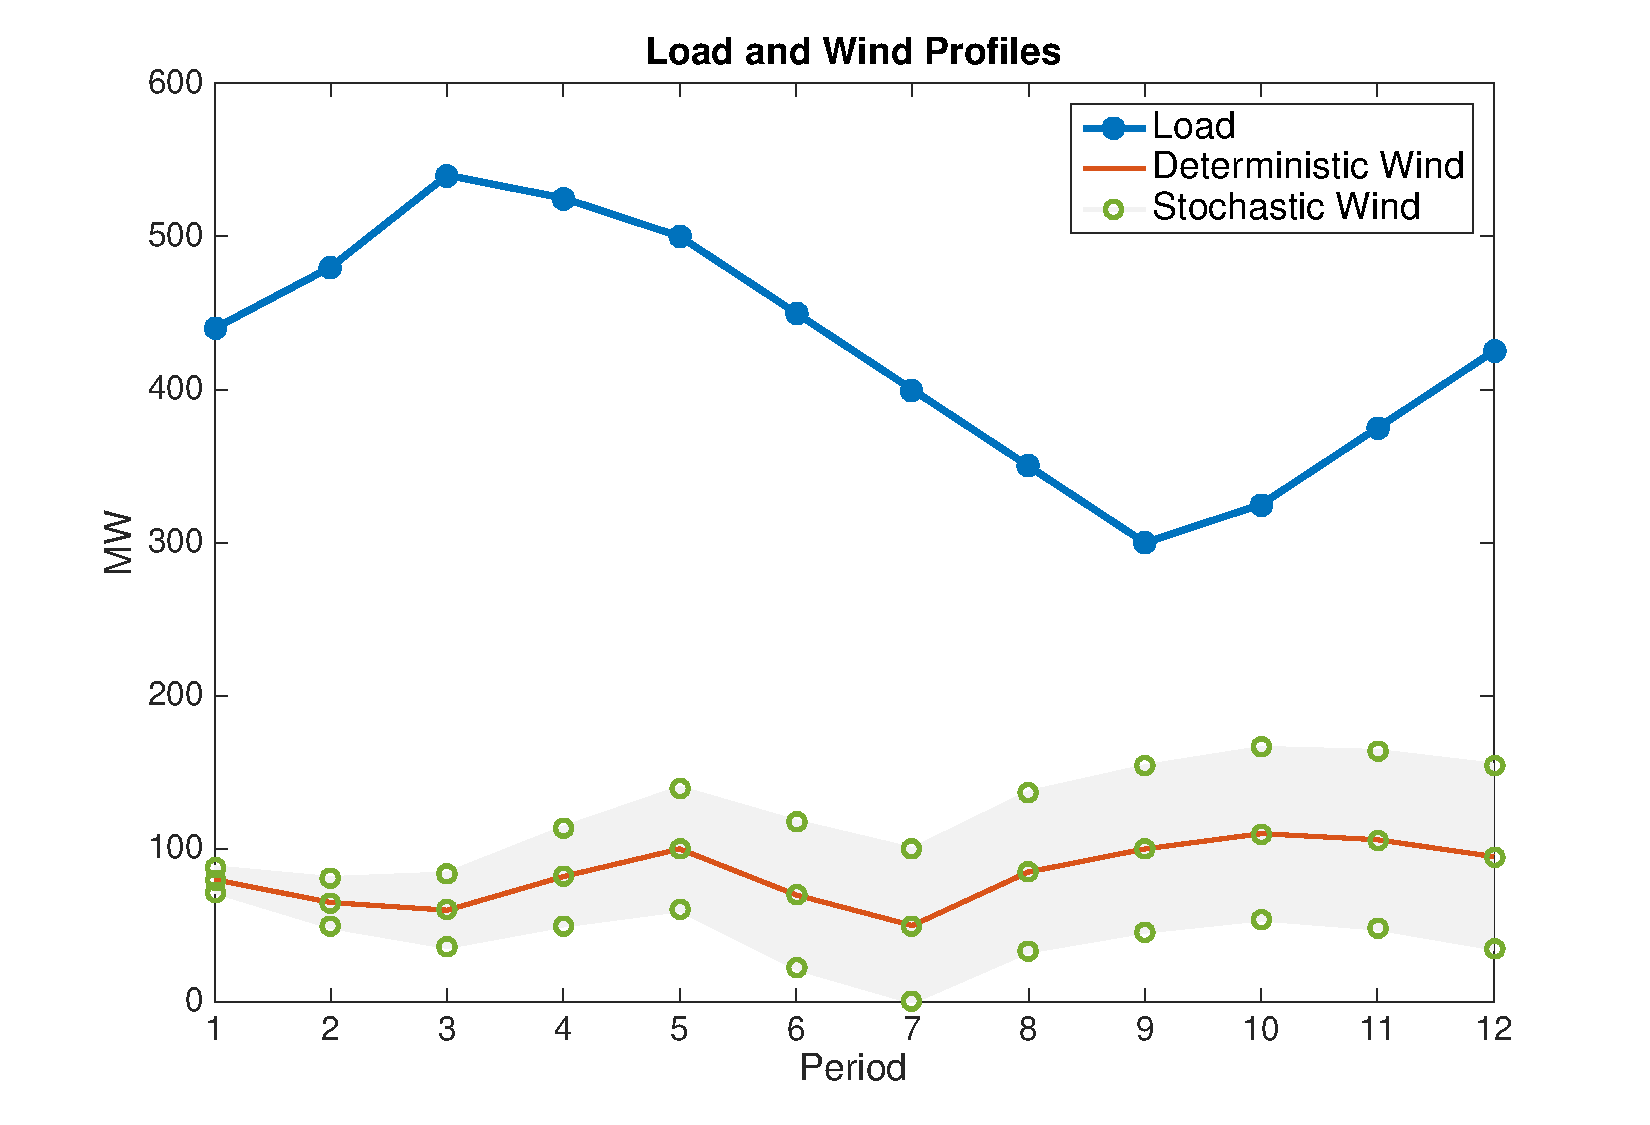
\includegraphics[width=\textwidth]{./figures/load_wind_profiles}
  \caption{Example Load and Wind Profiles}
  \label{fig:load_wind_profiles}
\end{figure}

\subsubsection{Example 5 -- Deterministic Multiperiod OPF}
\label{sec:tutex5}

This example illustrates a simple deterministic multiperiod DC OPF problem, where the dispatches in adjacent periods are linked by ramping constraints and costs.\footnote{The deterministic multiperiod DC OPF examples can be found in \code{most\_ex5\_mpopf.m}.} As described above, the variations to load and wind through the planning horizon are defined using profiles.

The \code{xGenData} is loaded from \code{ex\_xgd\_ramp.m}, which includes a \$10/MW cost on upward and downward ramping of generator~3 from one period to the next.
\begin{Code}
casefile = 'ex_case3b';
mpc = loadcase(casefile);
xgd = loadxgendata('ex_xgd_ramp', mpc);
[iwind, mpc, xgd] = addwind('ex_wind', mpc, xgd);
profiles = getprofiles('ex_wind_profile_d', iwind);
profiles = getprofiles('ex_load_profile', profiles);
nt = size(profiles(1).values, 1);       % number of periods
\end{Code}

The generator dispatches can be found in \code{mdo.flow(t).mpc.gen(:, PG)} for period $t$, or for all periods in the $n_g \times n_t$ matrix \code{mdo.results.ExpectedDispatch}.
\begin{Code}
mdi = loadmd(mpc, nt, xgd, [], [], profiles);
mdo = most(mdi, mpopt);
EPg = mdo.results.ExpectedDispatch;     % active generation
Elam = mdo.results.GenPrices;           % nodal energy price
most_summary(mdo);      % print results, depending on 'verbose' option
\end{Code}

The \code{RampWearCostCoeff} field of \code{xgd} is modified to add the wear and tear ramping costs from \eqref{eq:rampcost}. This can be done directly for an existing \code{xgd}, as shown below, or by adding a \code{RampWearCostCoeff} column in the \code{xGenData} file and defining the parameters there.
\begin{Code}
xgd.RampWearCostCoeff(1:3) = 1;
mdi = loadmd(mpc, nt, xgd, [], [], profiles);
mdo = most(mdi, mpopt);
EPg = mdo.results.ExpectedDispatch;     % active generation
Elam = mdo.results.GenPrices;           % nodal energy price
most_summary(mdo);      % print results, depending on 'verbose' option
\end{Code}

\subsubsection{Example 6 -- Deterministic Unit Commitment}
\label{sec:tutex6}

This example illustrates a deterministic unit commitment problem and how the commitment changes as more features are added.\footnote{The deterministic unit commitment examples can be found in \code{most\_ex6\_uc.m}. These example cases and the code used to produce the plots can also be found in the test file \code{t\_most\_uc.m}. Both files contain additional solver-specific options that you may find useful for these unit commitment examples.} These examples require a mixed-integer solver as described in Section~\ref{sec:sysreq} on System Requirements.

The \matpower{} case and \code{xGenData} for the full-featured example are loaded first and saved for later. Note that the \code{xGenData} here comes from \code{ex\_xgd\_uc.m} which includes \code{CommitKey} and activates the unit commitment formulation.
\begin{Code}
casefile = 'ex_case3b';
mpc = loadcase(casefile);
xgd = loadxgendata('ex_xgd_uc', mpc);
[iwind, mpc, xgd] = addwind('ex_wind_uc', mpc, xgd);
profiles = getprofiles('ex_wind_profile_d', iwind);
profiles = getprofiles('ex_load_profile', profiles);
nt = size(profiles(1).values, 1);       % number of periods
mpc_full = mpc;                         % save for later
xgd_full = xgd;                         % save for later
\end{Code}

\subsubsection*{Base : No Network}
This example begins with a simple sequence of economic dispatch problems, with no network constraints, no startup and shutdown costs, no minimum up or down time constraints, no ramp constraints or ramp reserve costs, and no storage. These features, except for storage, are already in included in the full model data loaded, so the first step is to remove these features to prepare for the first example. They will be added back in one at a time in the subsequent examples.
\begin{Code}
mpc.gencost(:, [STARTUP SHUTDOWN]) = 0; % remove startup/shutdown costs
xgd.MinUp(2) = 1;                       % remove min up-time constraint
xgd.PositiveLoadFollowReserveQuantity(3) = 250; % remove ramp reserve
xgd.PositiveLoadFollowReservePrice(3) = 1e-6;   % constraint and costs
xgd.NegativeLoadFollowReservePrice(3) = 1e-6;
\end{Code}
This model can then be run after turning off the DC network modeling. 
\begin{Code}
mpopt = mpoption(mpopt, 'most.dc_model', 0);    % use model with no network
mdi = loadmd(mpc, nt, xgd, [], [], profiles);
mdo = most(mdi, mpopt);
ms = most_summary(mdo);     % print results, depending on 'verbose' option
\end{Code}
The resulting commitment, dispatch and price schedules are shown in Figure~\ref{fig:uc_ex_1}. Notice that generator~3 only operates during hours 2, 3 and 4 and, as expected, the prices at all three buses are identical, since there is no network model to introduce transmission congestion.
\begin{figure}[hbtp]
  \centering
  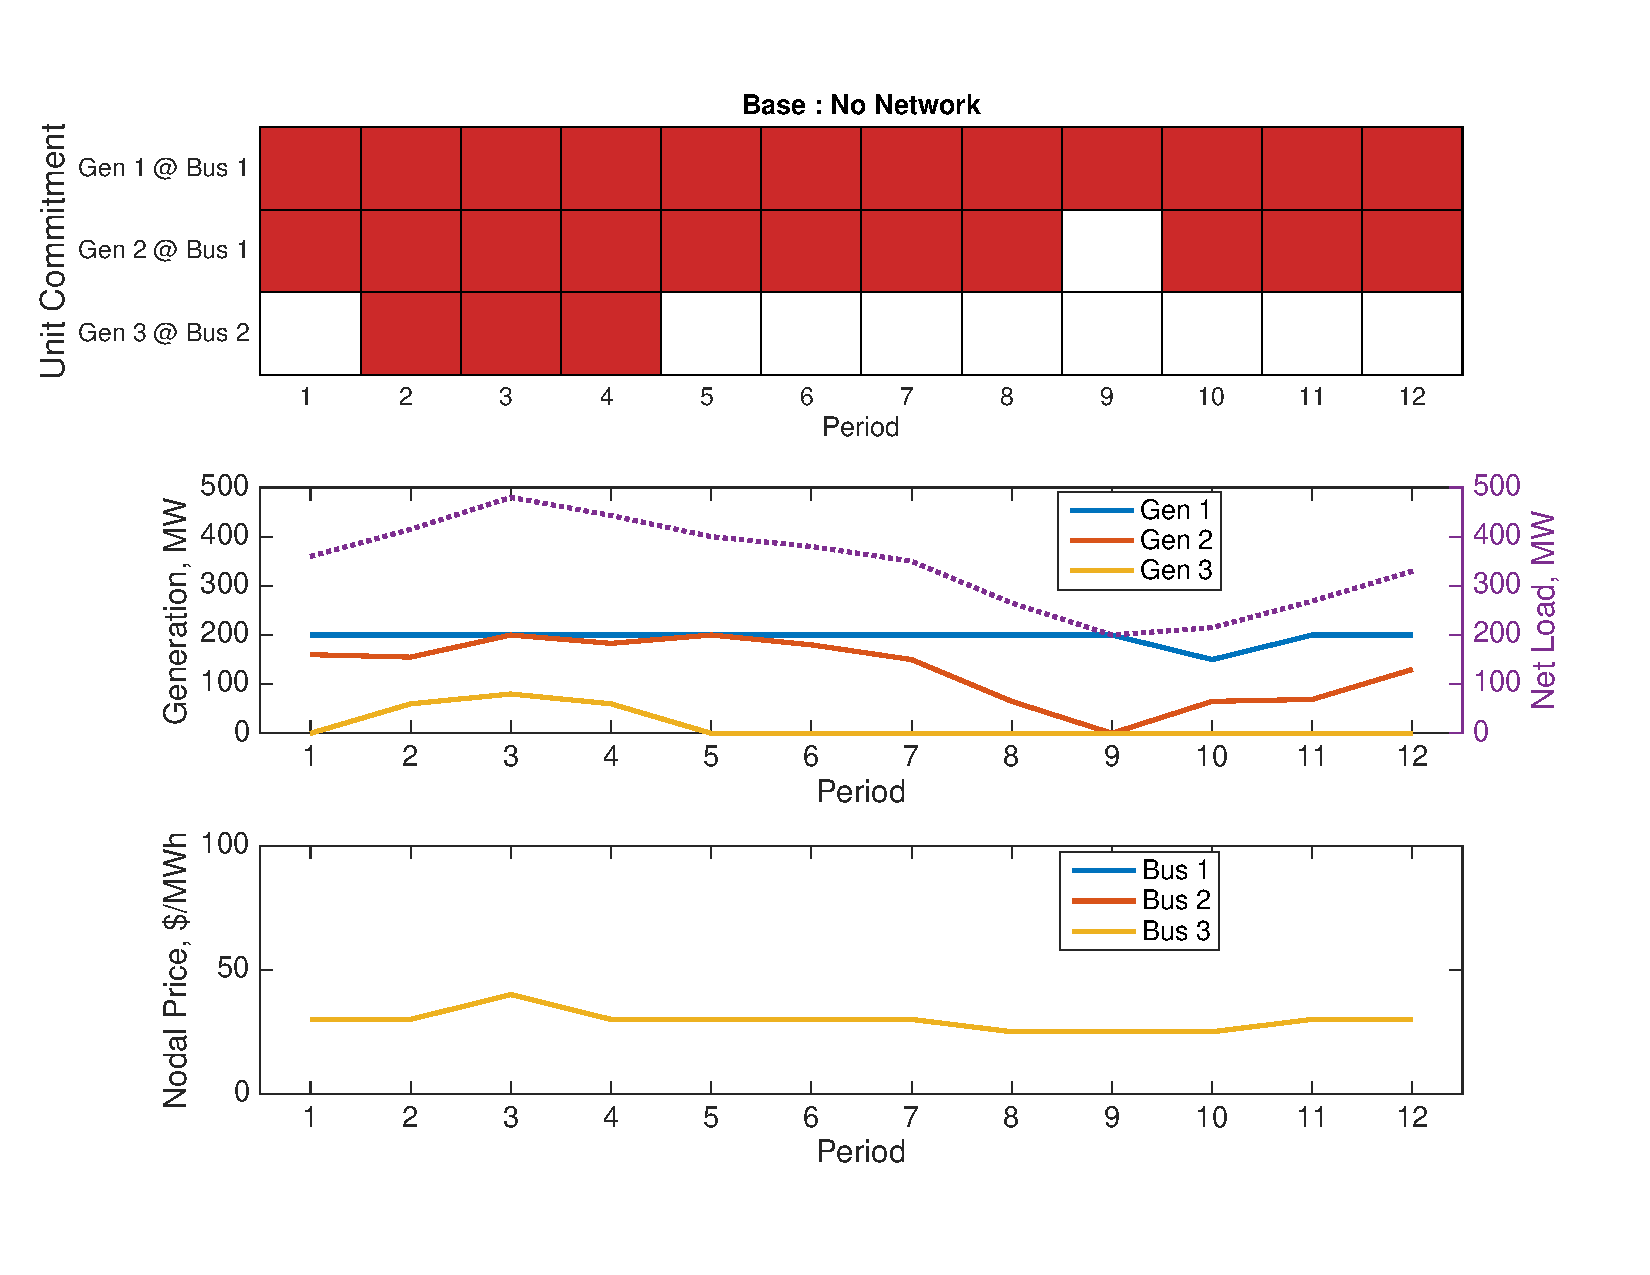
\includegraphics[width=\textwidth]{./figures/uc-ex-1}
  \caption{Deterministic UC : Base Case with No Network}
  \label{fig:uc_ex_1}
\end{figure}

\subsubsection*{Add DC Network Model}
If a DC network model is added, by simply toggling the \codeq{most.dc\_model} option and re-running the same model, the congestion in the line from bus~1 to bus~3 results in the nodal prices separating from one another and generator~3 carrying more of the load during the periods of higher net load, as seen in Figure~\ref{fig:uc_ex_2}.
\begin{Code}
mpopt = mpoption(mpopt, 'most.dc_model', 1);    % use DC network model (default)
mdo = most(mdi, mpopt);
\end{Code}
\begin{figure}[hbtp]
  \centering
  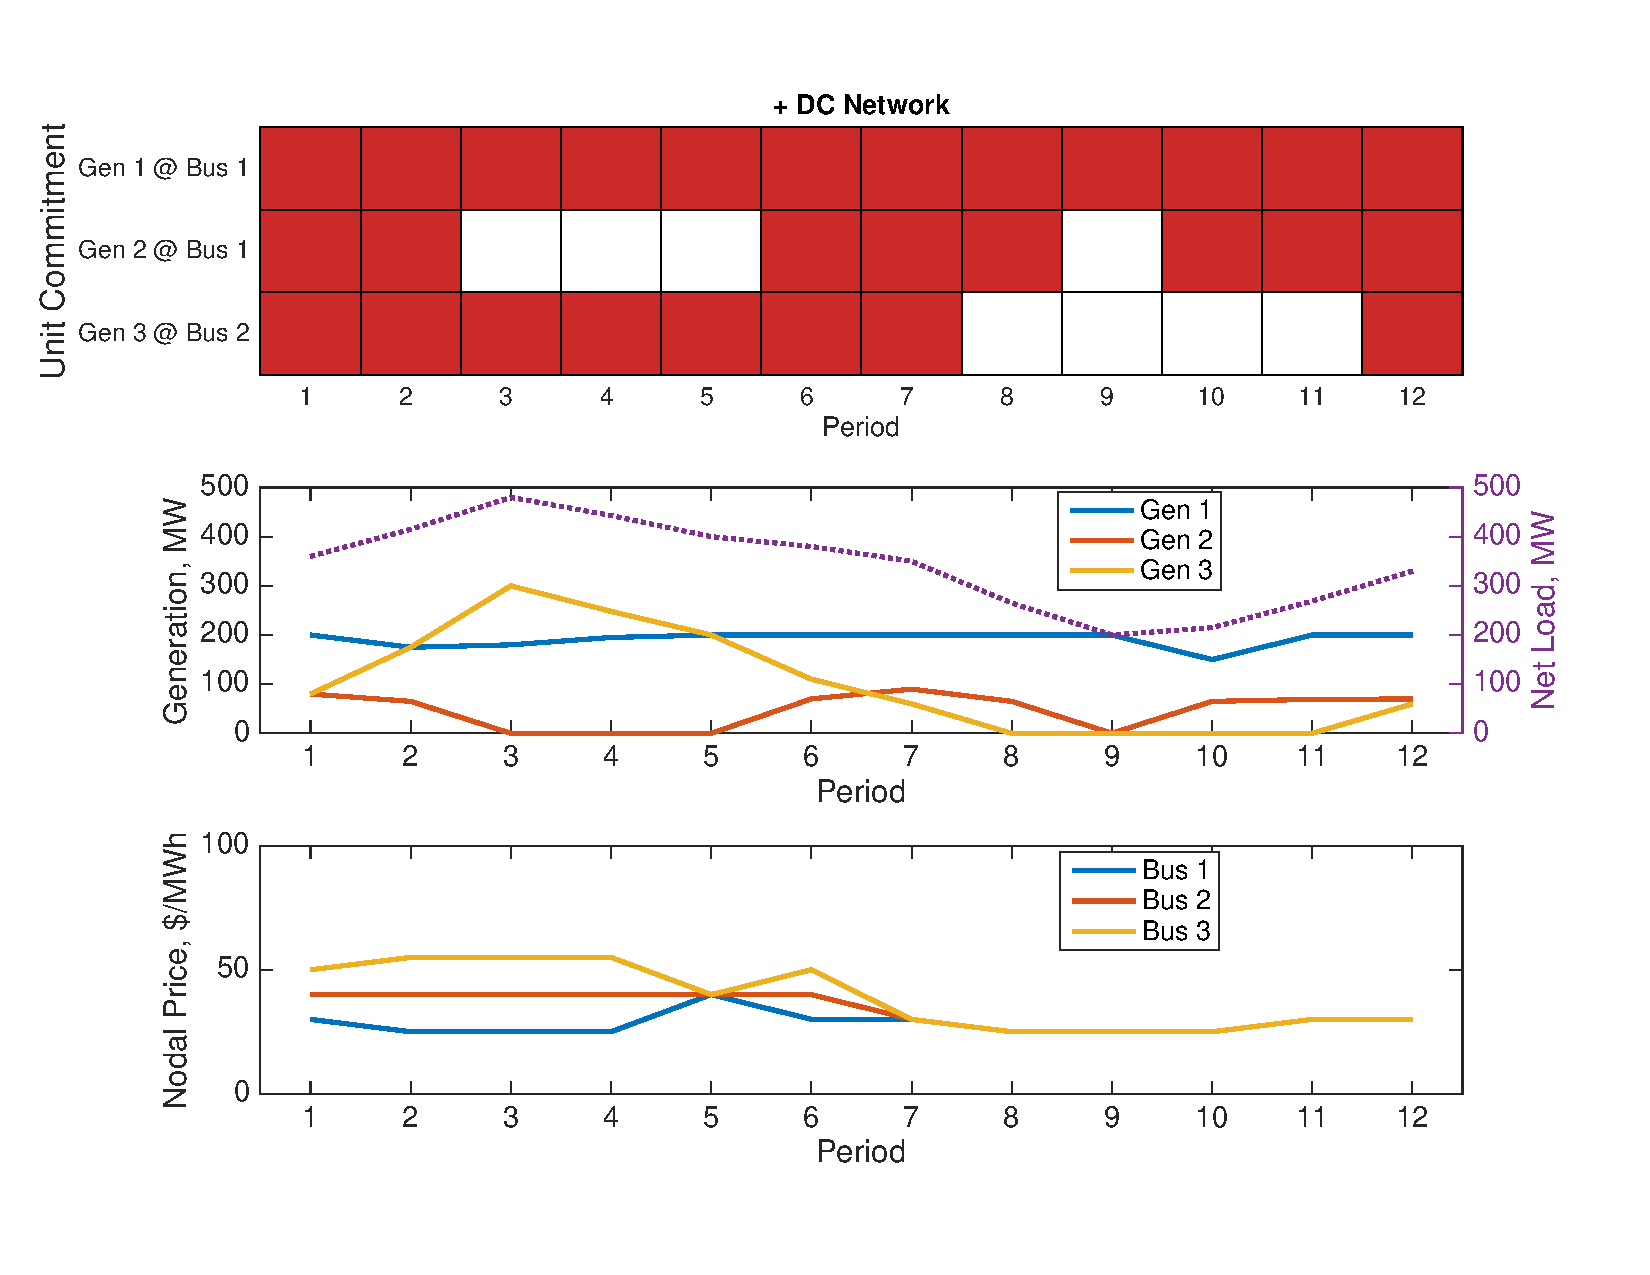
\includegraphics[width=\textwidth]{./figures/uc-ex-2}
  \caption{Deterministic UC : Add DC Network Model}
  \label{fig:uc_ex_2}
\end{figure}

\subsubsection*{Add Startup and Shutdown Costs}
To add startup and shutdown costs, restore the values from the original \matpower{} case and re-run.
\begin{Code}
mpc.gencost(2, [STARTUP SHUTDOWN]) = [ 200 200];
mpc.gencost(3, [STARTUP SHUTDOWN]) = [3000 600];
% equivalent to doing: mpc = mpc_full;
mdi = loadmd(mpc, nt, xgd, [], [], profiles);
mdo = most(mdi, mpopt);
\end{Code}
Notice in Figure~\ref{fig:uc_ex_3} that this results in generator~3 remaining on through the lower load hours, allowing generator~2 to stay off for hours 8--11.
\begin{figure}[hbtp]
  \centering
  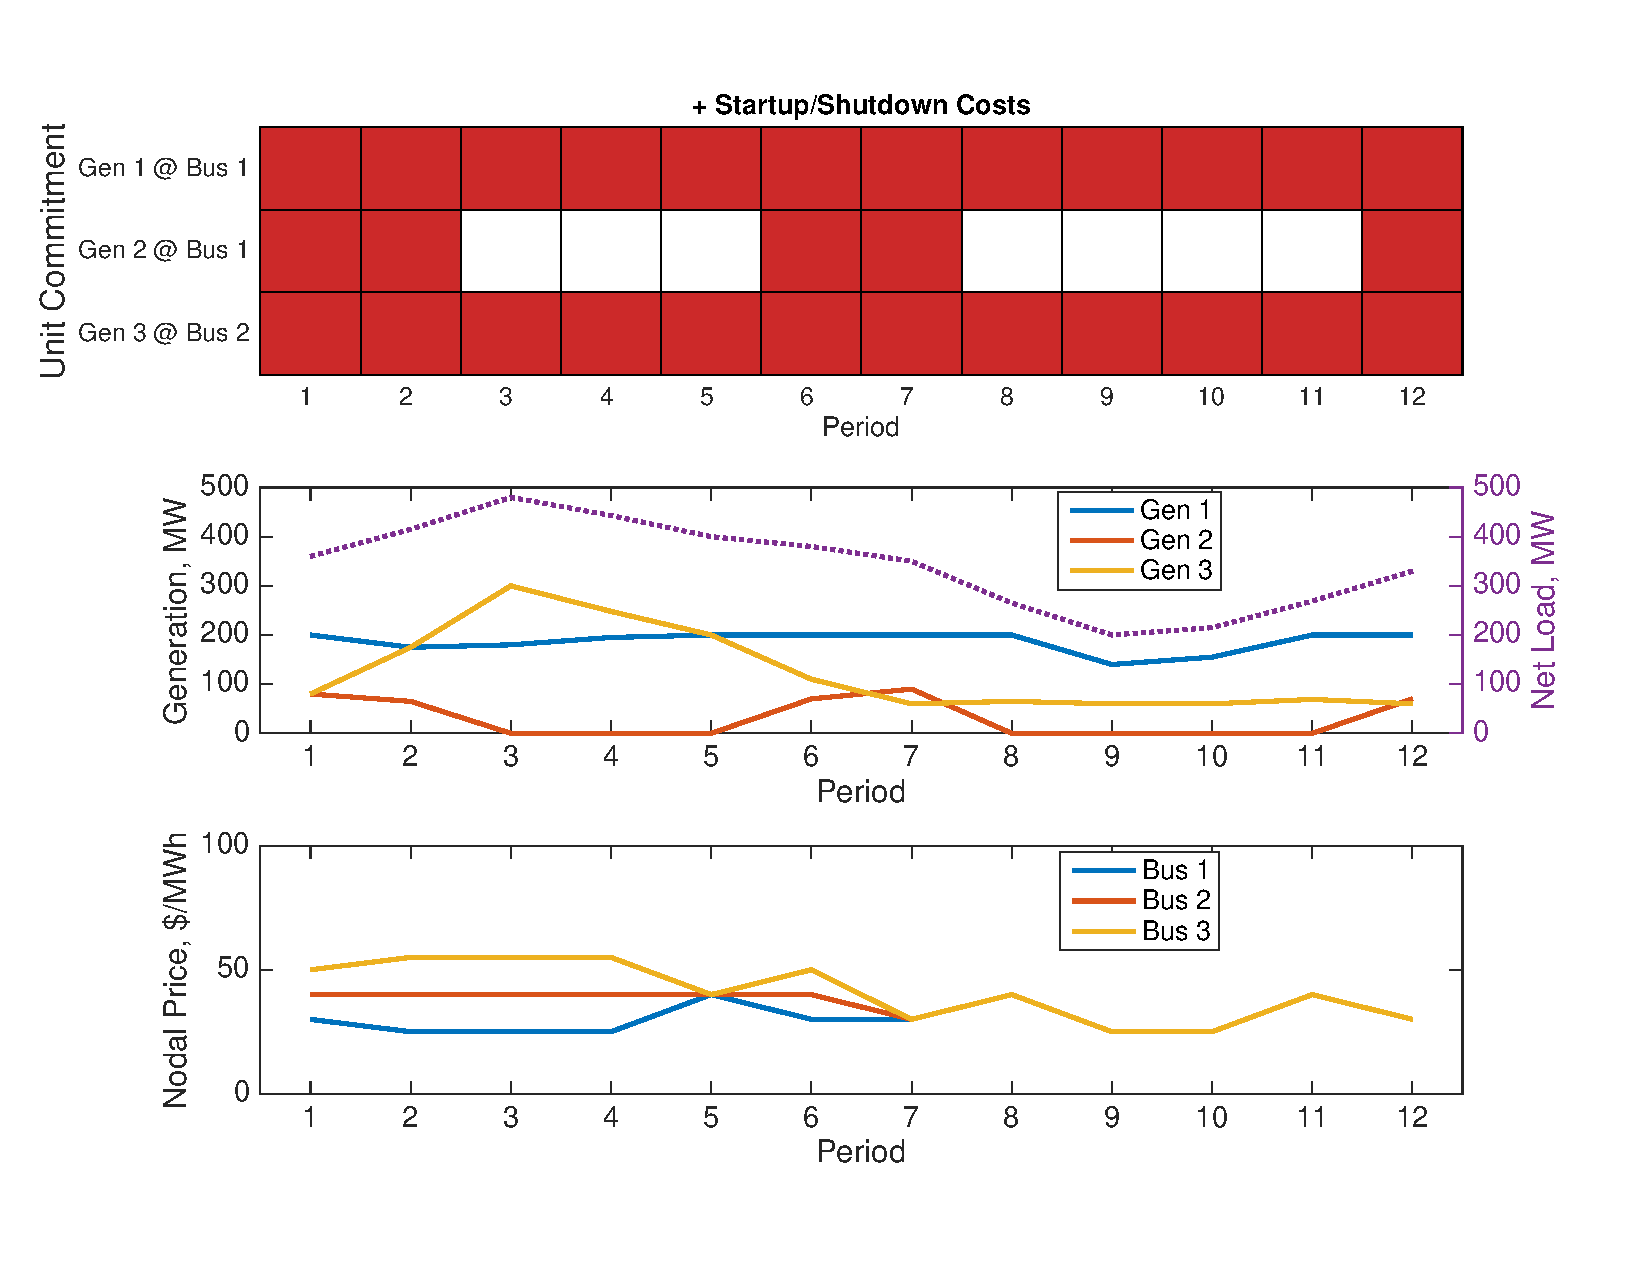
\includegraphics[width=\textwidth]{./figures/uc-ex-3}
  \caption{Deterministic UC : Add Startup and Shutdown Costs}
  \label{fig:uc_ex_3}
\end{figure}

\subsubsection*{Add Minimum Up and Down Time Constraints}
Notice in the previous example that the generator~2 is only running for two hours (6 and 7) in the middle of the planning horizon. Adding back the 3 hour minimum up-time constraint eliminates that solution.
\begin{Code}
xgd.MinUp(2) = 3;
mdi = loadmd(mpc, nt, xgd, [], [], profiles);
mdo = most(mdi, mpopt);
\end{Code}
Figure~\ref{fig:uc_ex_4} shows how this constraint results in starting up generator~2 an hour earlier (in period~5). Notice also that previously there was no network congestion in period~5, but starting generator~2 introduces congestion, causing the nodal prices in that period to separate from one another.
\begin{figure}[hbtp]
  \centering
  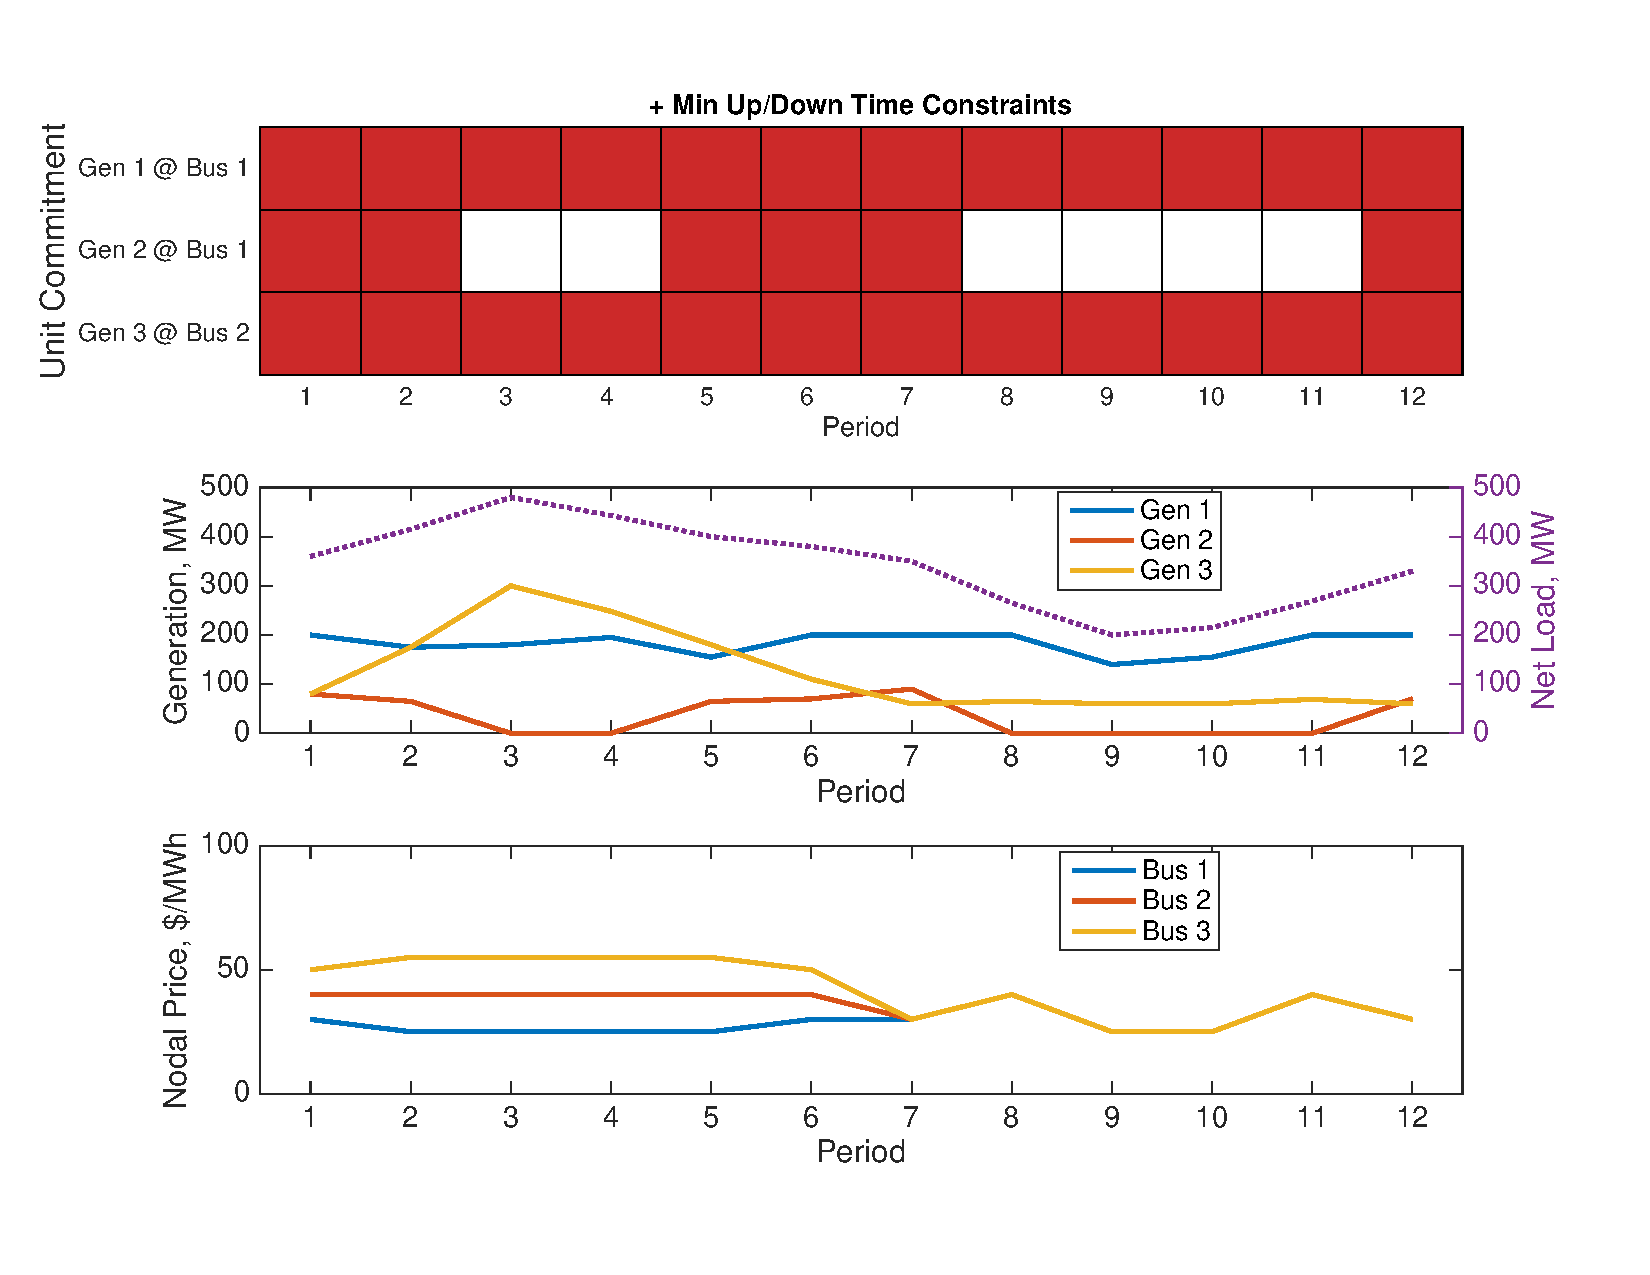
\includegraphics[width=\textwidth]{./figures/uc-ex-4}
  \caption{Deterministic UC : Add Min Up/Down Time Constraints}
  \label{fig:uc_ex_4}
\end{figure}

\subsubsection*{Add Ramping Constraints and Ramp Reserve Costs}
To add back the ramping constraints and ramp reserve costs, restore the values from the original \code{xGenData} and re-run.
\begin{Code}
xgd.PositiveLoadFollowReserveQuantity(3) = 100; % restore ramp reserve
xgd.PositiveLoadFollowReservePrice(3) = 10;     % constraint and costs
xgd.NegativeLoadFollowReservePrice(3) = 10;
% equivalent to doing: xgd = xgd_full;
mdi = loadmd(mpc, nt, xgd, [], [], profiles);
mdo = most(mdi, mpopt);
\end{Code}
Previously, generator~3 was ramping more than 200~MW from hour~1 to hour~3, which the newly added ramp constraint of 100~MW per hour precludes.
Figure~\ref{fig:uc_ex_5} shows that this fast ramp is reduced by shutting down generator~2 during the first two hours and starting generator~3 at a higher output level.
\begin{figure}[hbtp]
  \centering
  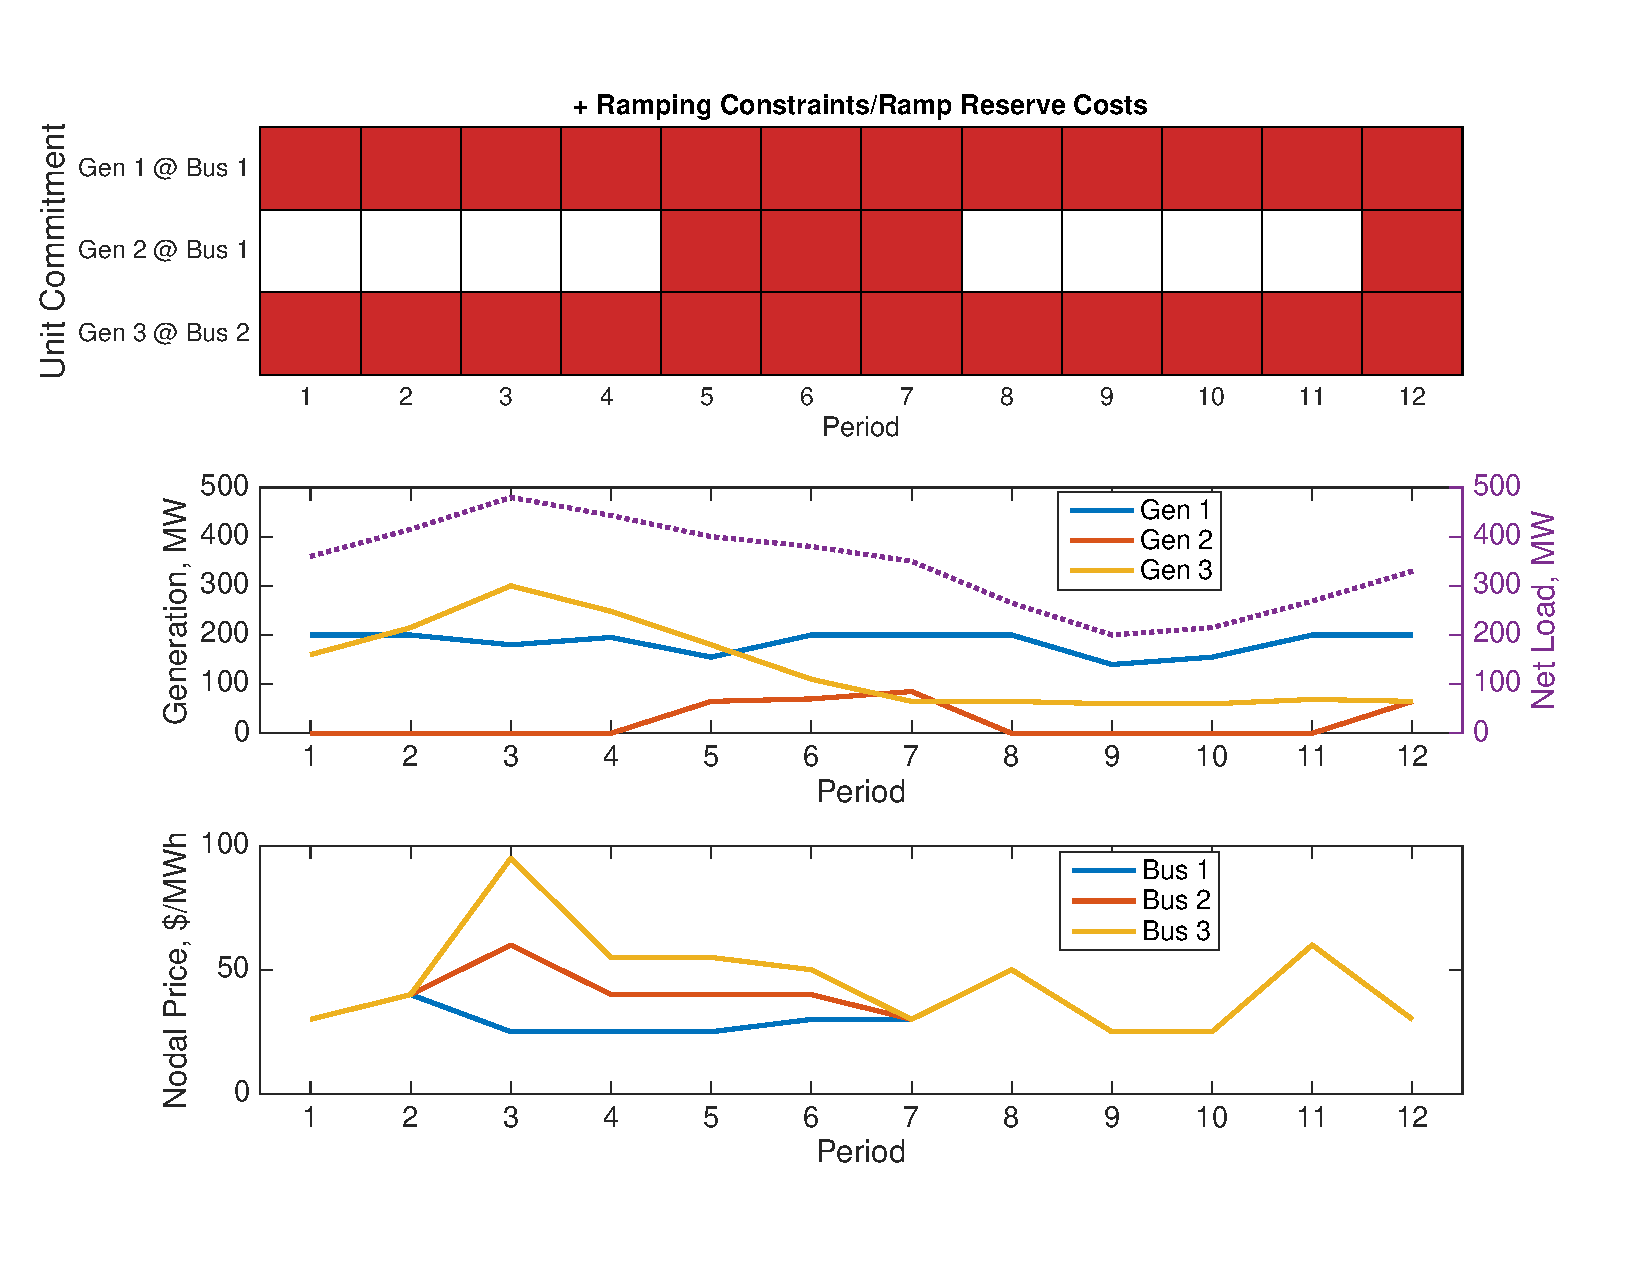
\includegraphics[width=\textwidth]{./figures/uc-ex-5}
  \caption{Deterministic UC : Add Ramp Constraints and Ramp Reserve Costs}
  \label{fig:uc_ex_5}
\end{figure}

\subsubsection*{Add Storage}
Finally, a 200~MWh storage unit is added at bus~3, as shown in the diagram in Figure~\ref{fig:threebus}. The magnitude of the power injection for this storage unit is limited to 80~MW, both for ``charging'' and ``discharging''. The cyclic storage constraint option is used to ensure that the stored energy at the end of the planning horizon is equal to the stored energy at the beginning.
\begin{Code}
mpopt = mpoption(mpopt, 'most.storage.cyclic', 1);
[iess, mpc, xgd, sd] = addstorage('ex_storage', mpc, xgd);
mdi = loadmd(mpc, nt, xgd, sd, [], profiles);
mdo = most(mdi, mpopt);
\end{Code}
Figure~\ref{fig:uc_ex_6} illustrates the effect of adding the storage unit. Since the unit is located at bus~3 with the load, it can reduce the congestion enough in peak hours to allow generator~2 to stay on for the full 12 hours. It also reduces the ramping capability required from the more expensive generator~3. As expected, the storage unit is charged during the periods of lower demand and lower price and discharged during the periods of higher demand and higher price.
\begin{figure}[hbt]
  \centering
  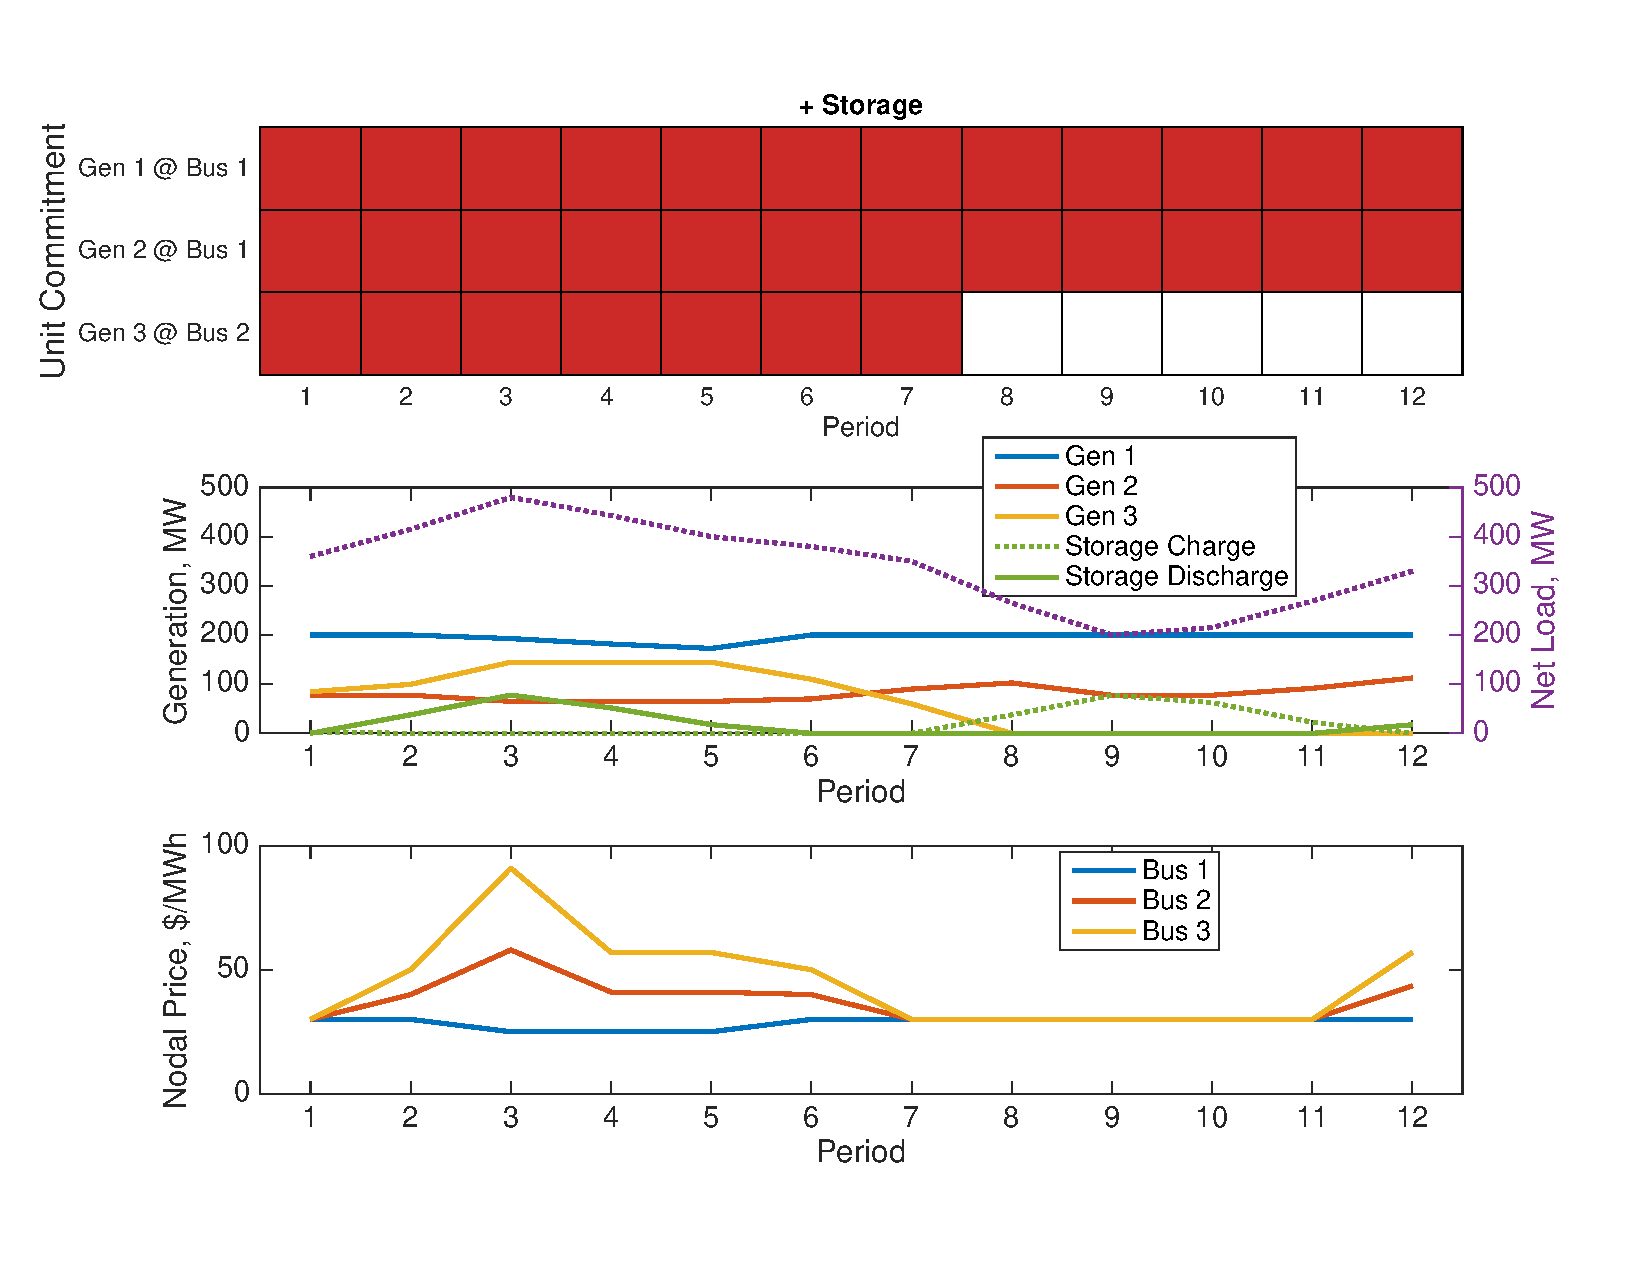
\includegraphics[width=\textwidth]{./figures/uc-ex-6}
  \caption{Deterministic UC : Add Storage}
  \label{fig:uc_ex_6}
\end{figure}


\subsubsection{Example 7 -- Secure Stochastic Unit Commitment}
\label{sec:tutex7}

The following examples are based on example~6 above, with all of the features, except storage, included. Instead of deterministic wind, however, a stochastic model of wind is assumed.\footnote{The secure and stochastic unit commitment examples can be found in \code{most\_ex7\_suc.m}. These example cases and the code used to produce the plots can also be found in the test file \code{t\_most\_suc.m}.} In these examples, three samples of wind availability serve as the base scenarios, representing low, average and high wind realizations. These wind scenarios are defined in \code{ex\_wind\_profile.m}. In this case, since there is a single load profile defined in \code{ex\_load\_profile.m}, it is automatically expanded to apply to all three wind scenarios as well. The examples in this section all use the following setup.
\begin{Code}
mpc = loadcase('ex_case3b');
xgd = loadxgendata('ex_xgd_uc', mpc);
[iwind, mpc, xgd] = addwind('ex_wind_uc', mpc, xgd);
profiles = getprofiles('ex_wind_profile', iwind);
profiles = getprofiles('ex_load_profile', profiles);
nt = size(profiles(1).values, 1);       % number of periods
nj = size(profiles(1).values, 2);       % number of scenarios
\end{Code}

\subsubsection*{Stochastic Unit Commitment -- Individual Trajectories}

The \code{transmat} argument to \code{loadmd} defines the probabilities of transitions from the scenarios in period~$t-1$ to the scenarios in period~$t$. If identity matrices are used for these transition probabilities, this results in the special case in which there are 3 full trajectories through the horizon, each of which can be viewed as a different ``scenario''. That is, if the system is in the high wind state in the first period, it will stay in the high wind state in every subsequent period, and the same with the average and low wind states. Figure~\ref{fig:wind_profile_1} illustrates this special case.
\begin{figure}[hbtp]
  \centering
  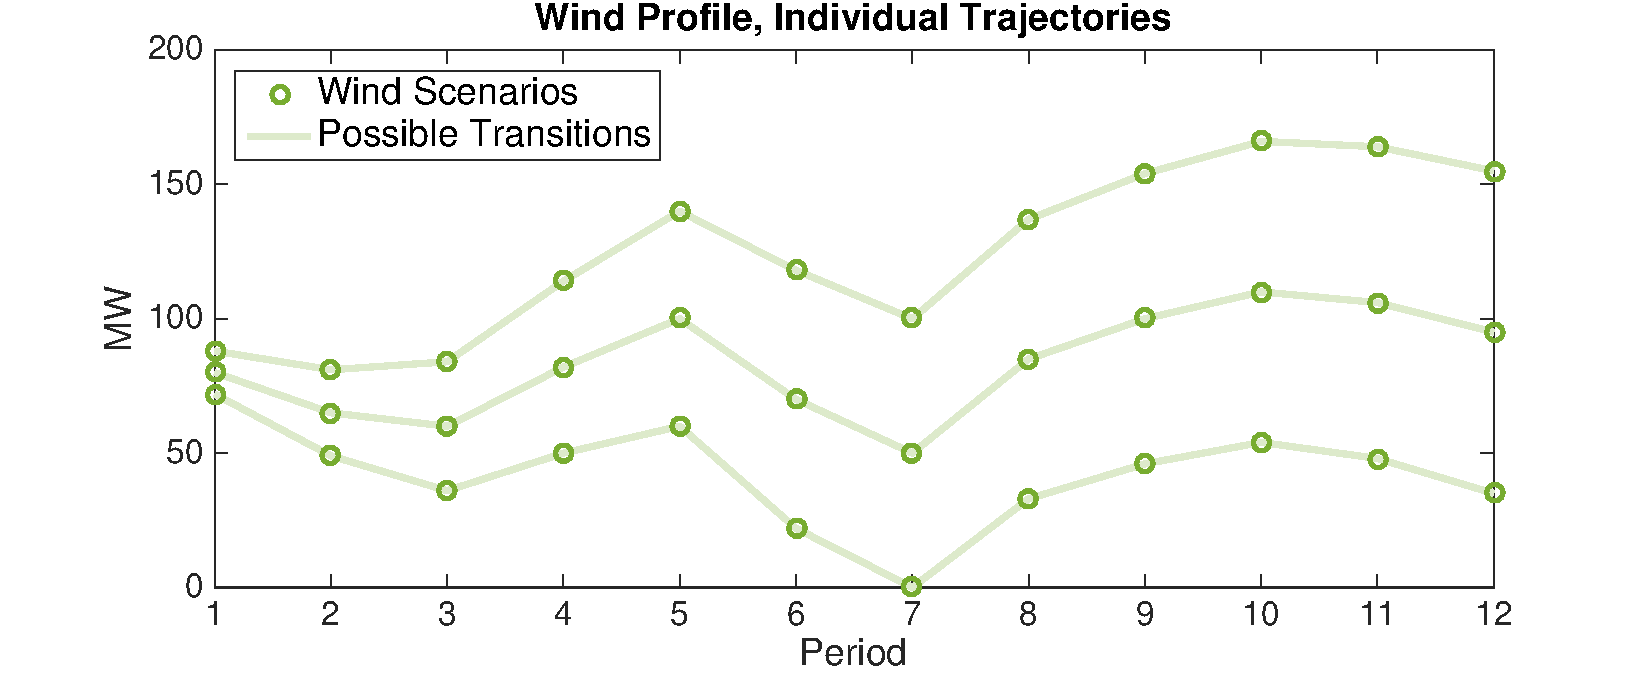
\includegraphics[width=\textwidth]{./figures/wind_profile_1}
  \caption{Example Wind Profiles, Individual Trajectories}
  \label{fig:wind_profile_1}
\end{figure}

In this case, it is also necessary to define the binary valued mask $\zeta^{tj_2j_1}$ in \eqref{eq:rampconstrdef} so that the ramp reserve constraints \eqref{eq:inter1}--\eqref{eq:rampconstr} only include the transitions with non-zero probability. This is done using the \code{filter\_ramp\_transitions} function.\footnote{See Section~\ref{sec:filter_ramp_transitions}.}
\begin{Code}
transmat = cell(1, nt);
I = speye(nj);
[transmat{:}] = deal(I);
transmat{1} = [0.16; 0.68; 0.16];   % period 1 probabilities
mdi = loadmd(mpc, transmat, xgd, [], [], profiles);
mdi = filter_ramp_transitions(mdi, 0.1);
mdo = most(mdi, mpopt);
ms = most_summary(mdo);
\end{Code}
The resulting unit commitment, expected dispatch and price schedules are shown in Figure~\ref{fig:suc_ex_2}.
\begin{figure}[hbtp]
  \centering
  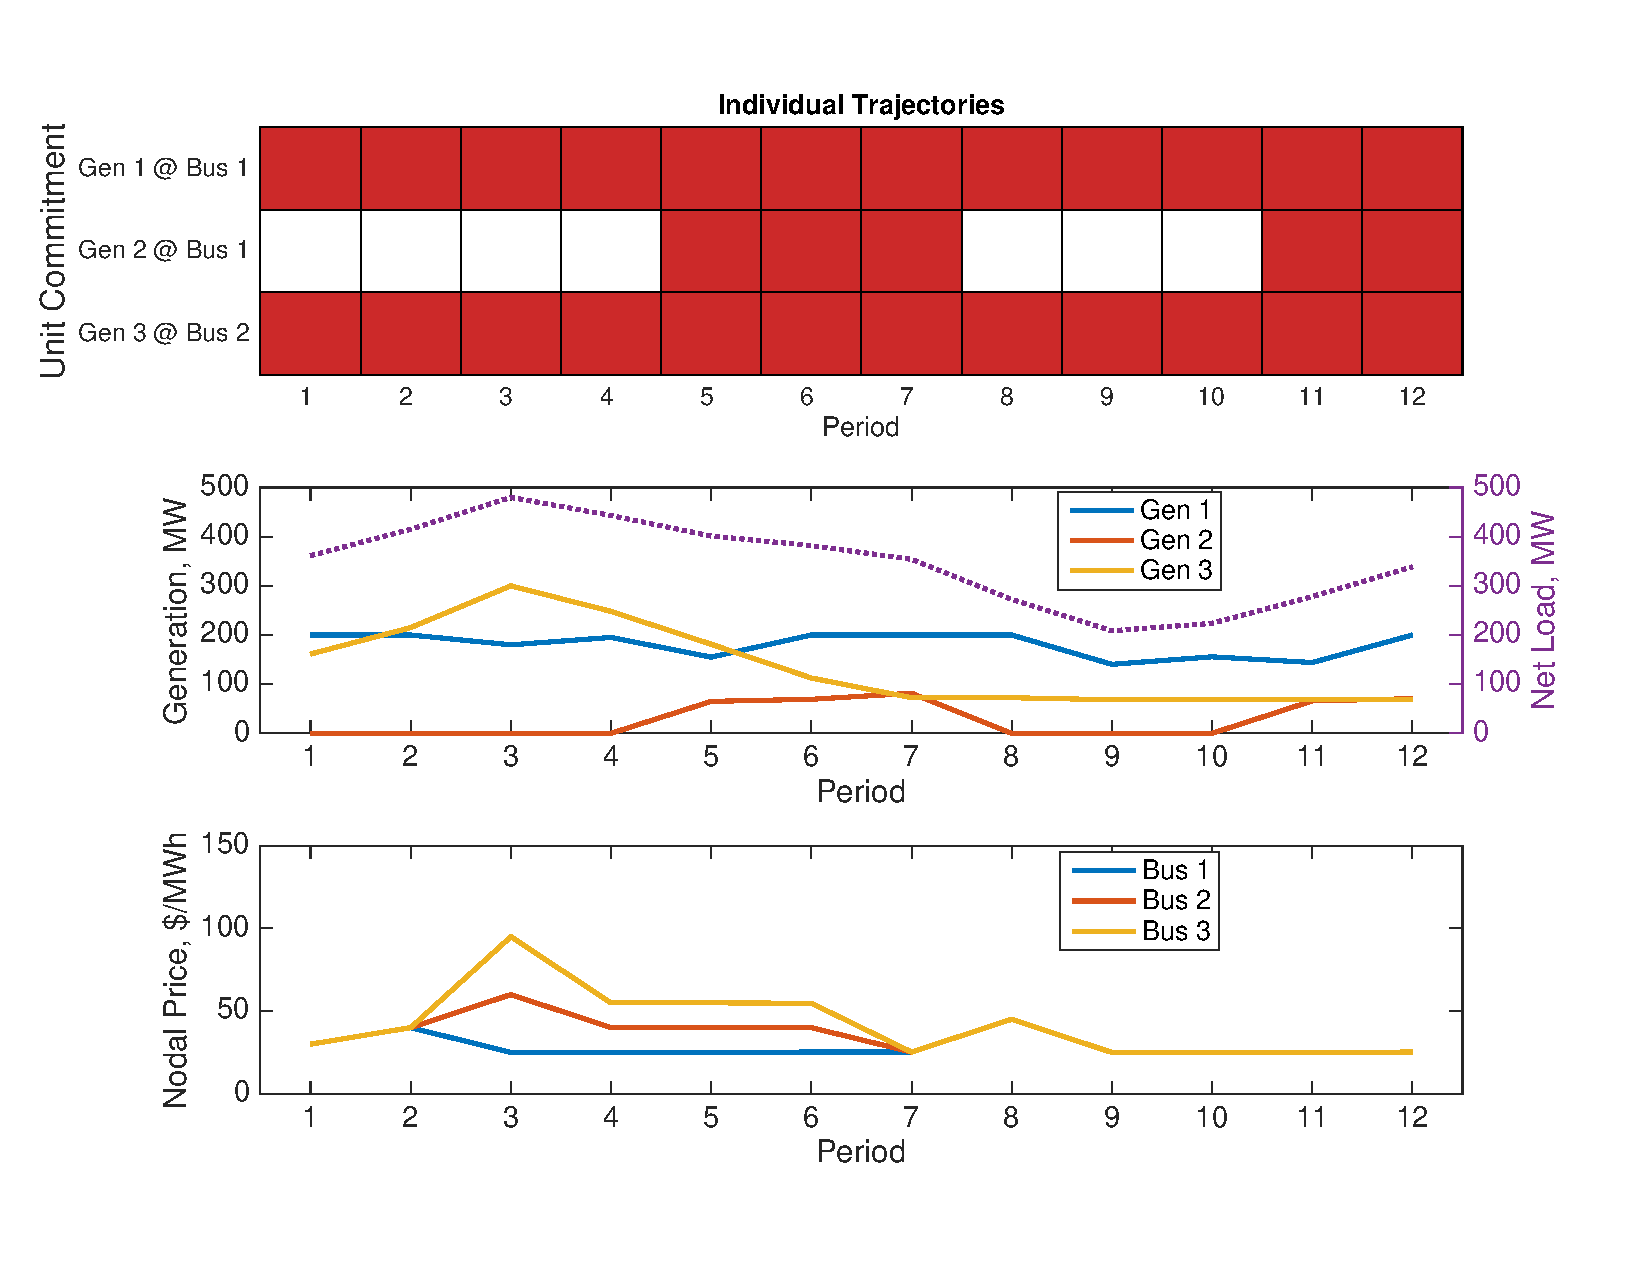
\includegraphics[width=\textwidth]{./figures/suc-ex-2}
  \caption{Stochastic UC : Individual Trajectories}
  \label{fig:suc_ex_2}
\end{figure}

\subsubsection*{Stochastic Unit Commitment -- Full Transition Probabilities}

The more general case of stochastic unit commitment implemented by \most{} uses  full transition probability matrices, where transitions between low, average and high wind scenarios are allowed from period to period as illustrated in Figure~\ref{fig:wind_profile_2}. In this case the binary valued mask $\zeta^{tj_2j_1}$ is left at its default value of all ones, resulting in ramp reserve constraints that encompass the largest period to period ramps.
\begin{figure}[hbtp]
  \centering
  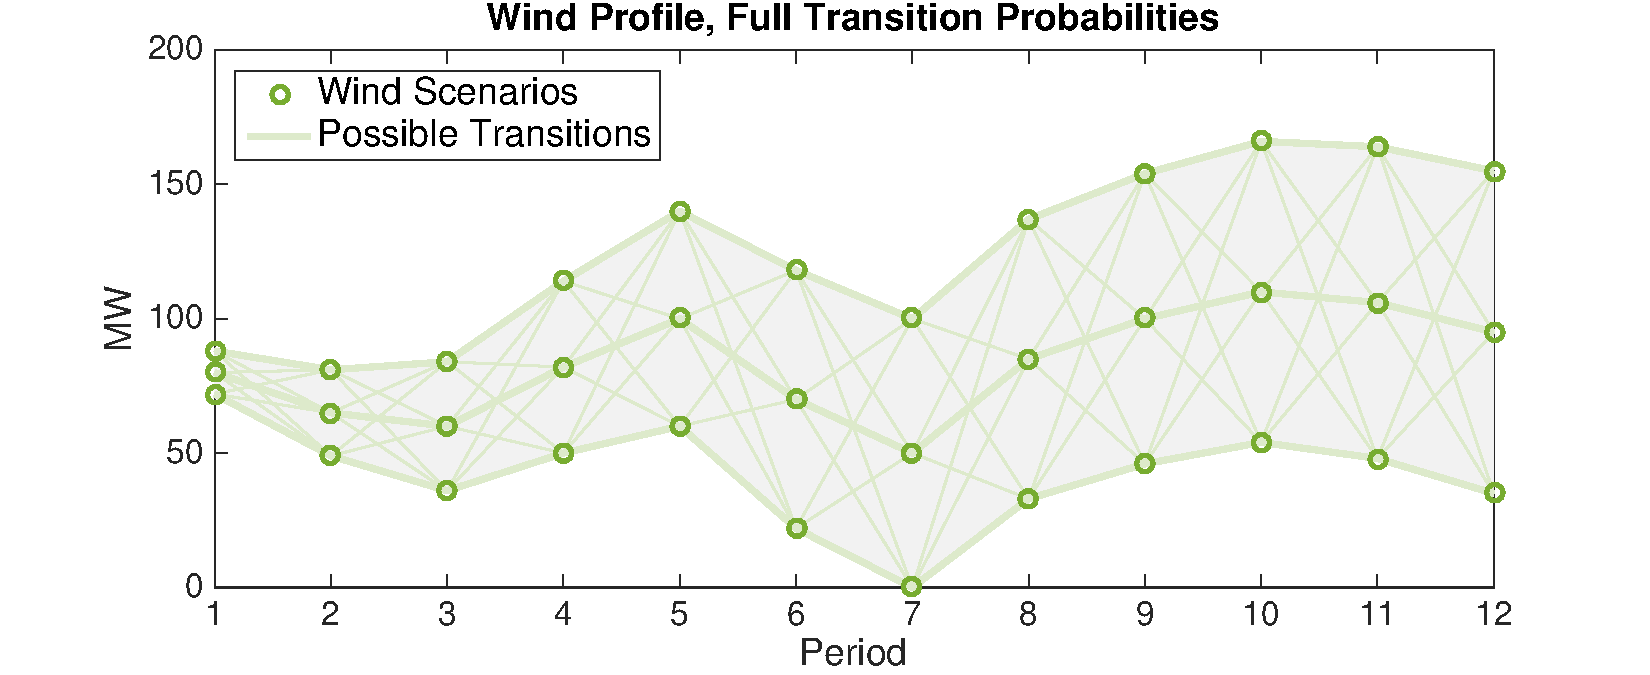
\includegraphics[width=\textwidth]{./figures/wind_profile_2}
  \caption{Example Wind Profiles, Full Transition Probabilities}
  \label{fig:wind_profile_2}
\end{figure}
\begin{Code}
transmat = ex_transmat(nt);
mdi = loadmd(mpc, transmat, xgd, [], [], profiles);
mdo = most(mdi, mpopt);
ms = most_summary(mdo);
\end{Code}
This case results in a different unit commitment as seen in Figure~\ref{fig:suc_ex_3}, where generator~2 remains on throughout the later hours.
\begin{figure}[hbtp]
  \centering
  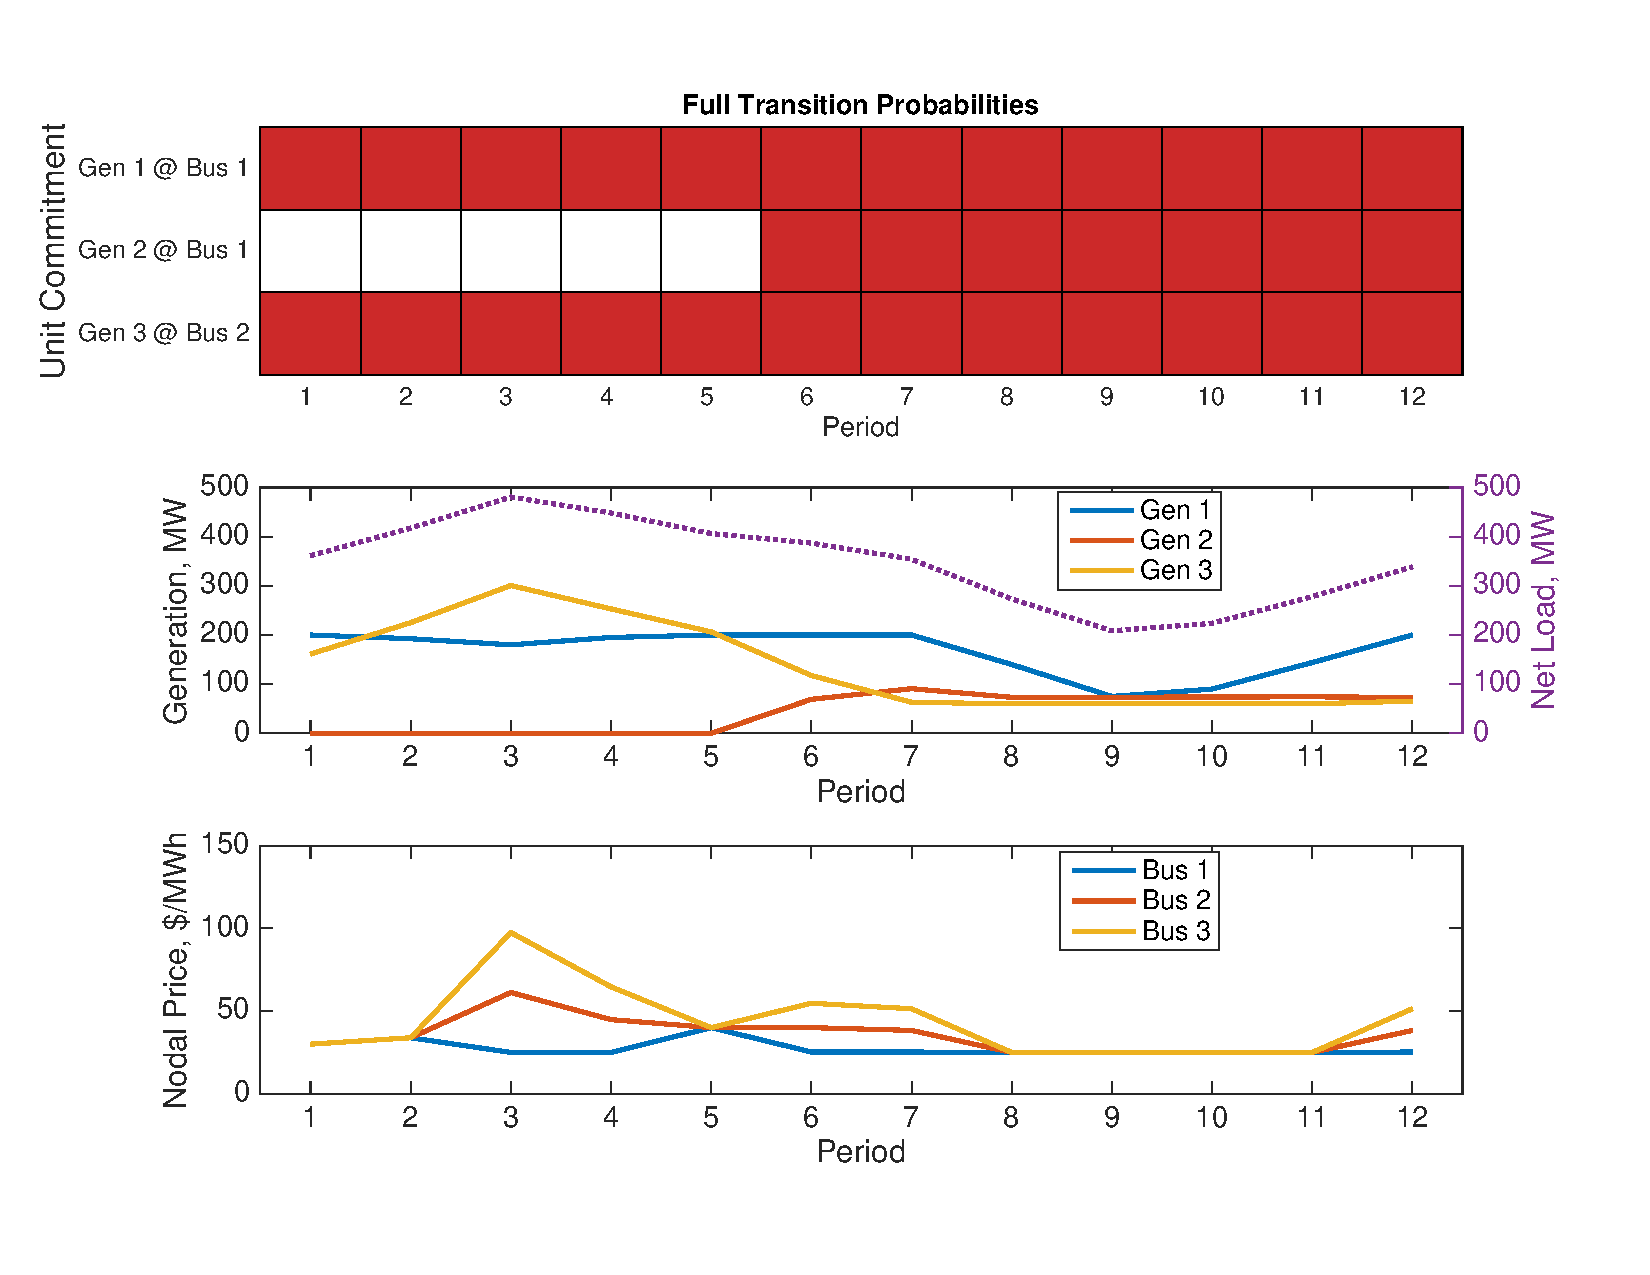
\includegraphics[width=\textwidth]{./figures/suc-ex-3}
  \caption{Stochastic UC : Full Transition Probabilities}
  \label{fig:suc_ex_3}
\end{figure}

\subsubsection*{Secure Stochastic Unit Commitment}

This example uses the general full transition probabilities and also includes contingencies for security in each period.
\begin{Code}
transmat = ex_transmat(nt);
mdi = loadmd(mpc, transmat, xgd, [], 'ex_contab', profiles);
mdo = most(mdi, mpopt);
ms = most_summary(mdo);
\end{Code}
Figure~\ref{fig:suc_ex_4} shows the resulting unit commitment, expected dispatch and pricing scheules.
\begin{figure}[hbtp]
  \centering
  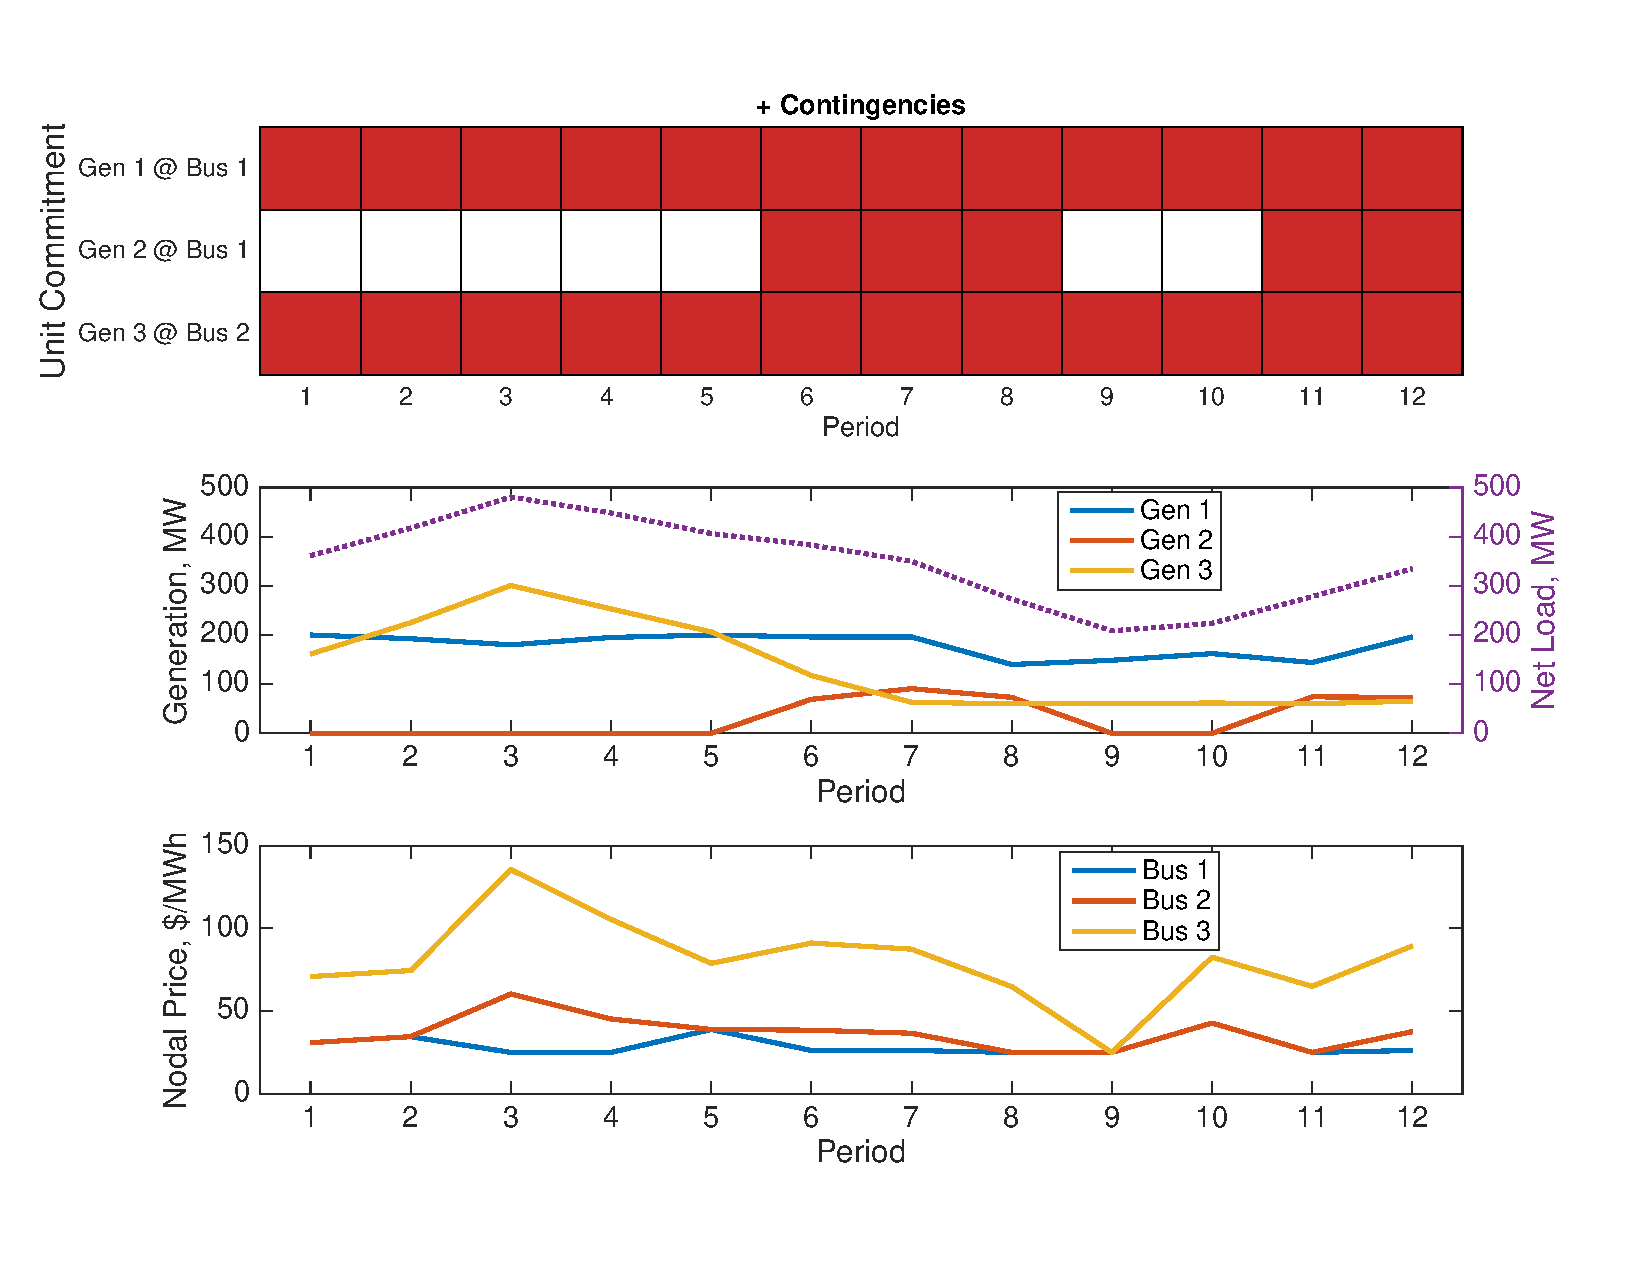
\includegraphics[width=\textwidth]{./figures/suc-ex-4}
  \caption{Secure Stochastic UC : Full Transition Probabilities + Contingencies}
  \label{fig:suc_ex_4}
\end{figure}


\subsubsection*{Secure Stochastic Unit Commitment with Storage}

Finally, a storage unit is added to the system, yielding a case that utilizes the majority of the features of the \most{} formulation.

\begin{Code}
transmat = ex_transmat(nt);
[iess, mpc, xgd, sd] = addstorage('ex_storage', mpc, xgd);
mdi = loadmd(mpc, transmat, xgd, sd, 'ex_contab', profiles);
mdo = most(mdi, mpopt);
ms = most_summary(mdo);
\end{Code}
As seen in Figure~\ref{fig:suc_ex_5}, the storage allows all units to remain on for the entire horizon, avoiding the startup and shutdown costs.
\begin{figure}[hbtp]
  \centering
  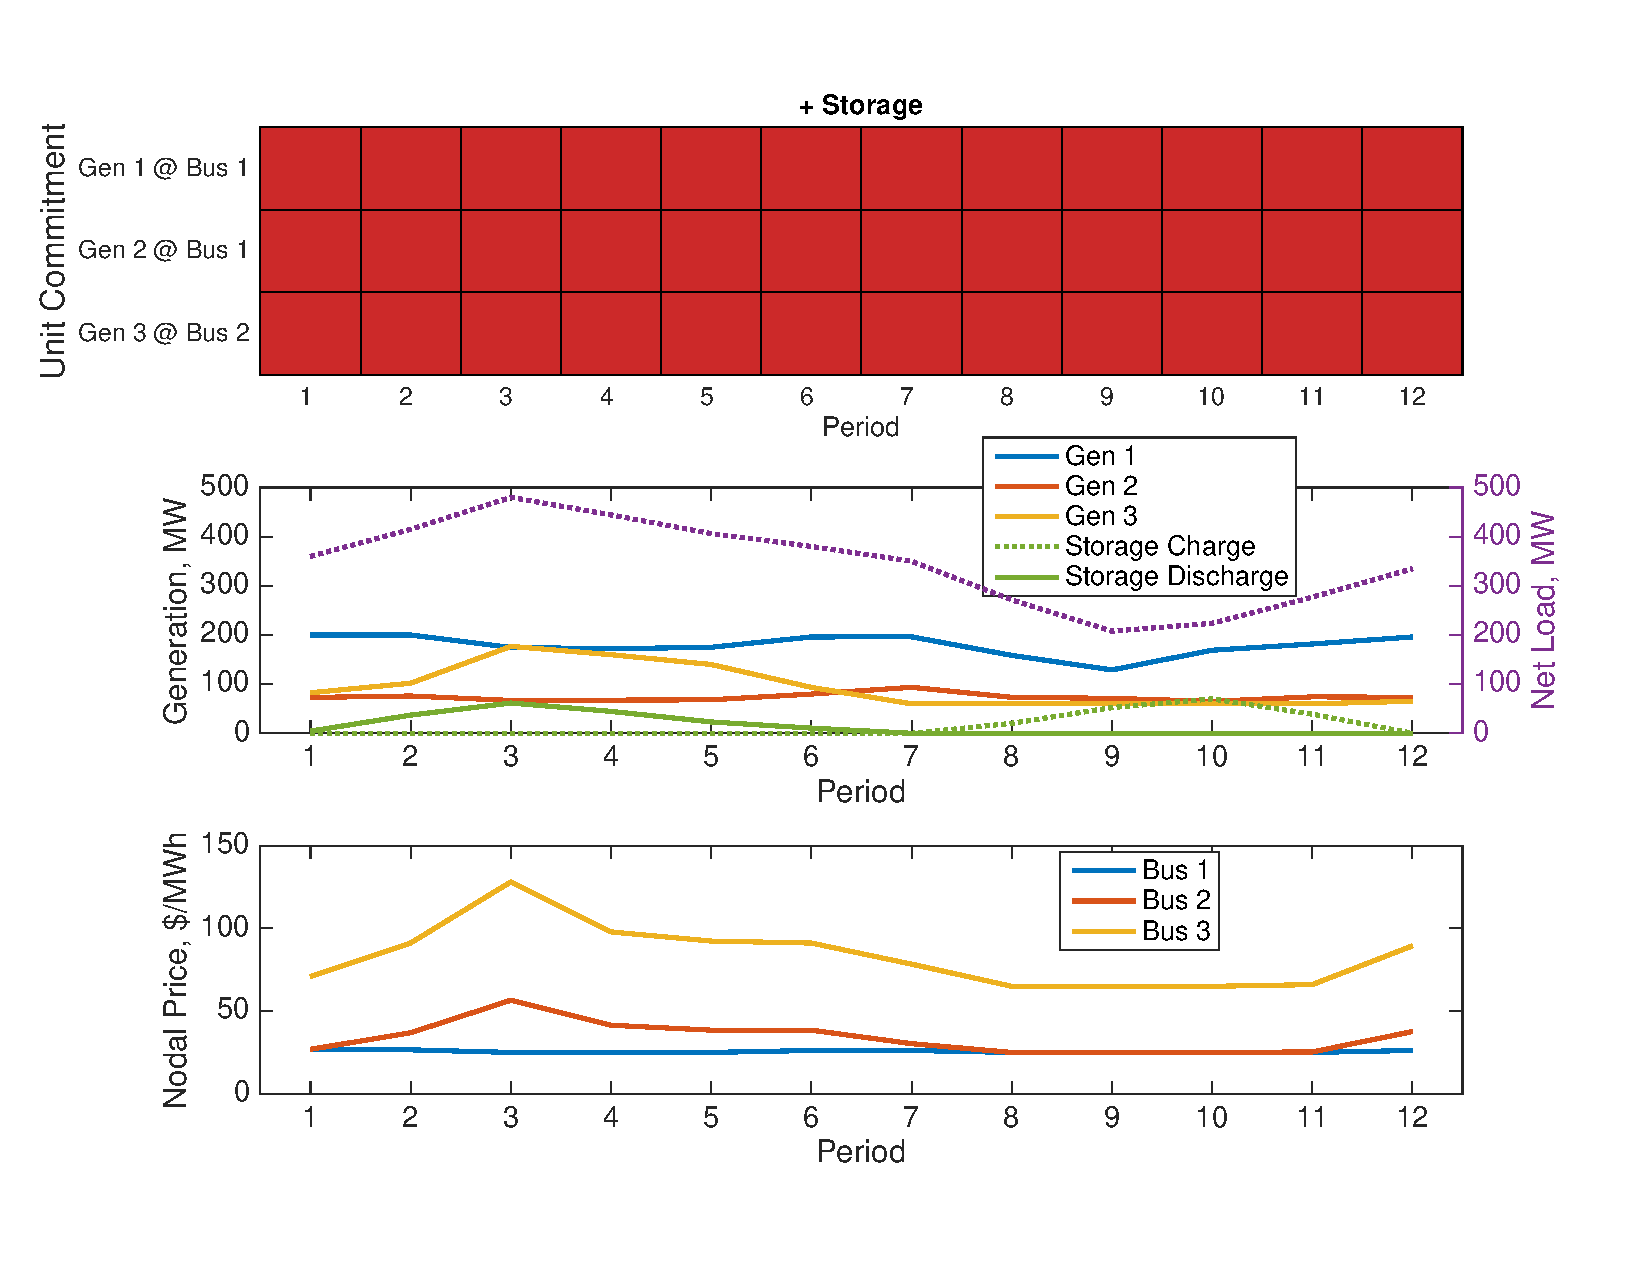
\includegraphics[width=\textwidth]{./figures/suc-ex-5}
  \caption{Secure Stochastic UC with Storage}
  \label{fig:suc_ex_5}
\end{figure}

\subsubsection{Dynamical System Constraint Example}
\label{sec:ds_ex}

An example of using the linear time-varying dynamical system constraints can be found in \code{t\_most\_w\_ds.m}.


%%------------------------------------------
\clearpage
\section{Acknowledgments}

This work was supported in part by the \CERTS{} and the Office of Electricity Delivery and Energy Reliability, Transmission Reliability Program of the U.S. Department of Energy under the National Energy Technology Laboratory Cooperative Agreement No.~DE-FC26-09NT43321.

The authors would like to thank the following people, in no particular order, for their various contributions to \most{} and the SuperOPF project upon which it is based: Robert~J. Thomas, Timothy~D. Mount, C.~Lindsay Anderson, Alberto Lamadrid, Daniel Mu\~noz-\'Alvarez, James~S. Thorp, William~D. Schulze, Jie Chen, Hongye Wang, Wooyoung Jeon and Surin Maneevitjit.

%\appendix
%\appendixpage
%\addappheadtotoc

\begin{appendices}

% %%------------------------------------------
% \clearpage
% \section{\most{} Options}
% \label{app:options}


%%------------------------------------------
\clearpage
\section{\most{} Files and Functions}
\label{app:functions}

This appendix lists all of the files and functions that \most{} provides. In most cases, the function is found in a \matlab{} M-file of the same name in the \code{lib} directory of the \most{} distribution\footnote{That is, in the \mostpath{/lib} directory.}, where the \code{.m} extension is omitted from this listing. For more information on each, at the \matlab{} prompt, simply type \code{help} followed by the name of the function. For documentation and data files, the filename extensions are included.


\subsection{\most{} Documentation Files}

\begin{table}[!ht]
%\renewcommand{\arraystretch}{1.2}
\centering
\begin{threeparttable}
\caption{\most{} Documentation Files}
\label{tab:mostdocfiles}
\footnotesize
\begin{tabular}{lp{0.6\textwidth}}
\toprule
name & description \\
\midrule
\code{docs/}	& \most{} documentation	\\
\code{~~MOST-manual.pdf}	& \mostman{}	\\
\code{~~src/}	& \LaTeX{} source for \mostman{}	\\
\code{lib/}	& \most{} software (see Table~\ref{tab:mostsw})	\\
\code{~~t/}	& \most{} tests and examples (see Tables~\ref{tab:mosttestdata} and \ref{tab:mosttests})	\\
\code{AUTHORS}	& list of \most{} authors	\\
\code{CHANGES.md}	& \most{} change history	\\
\code{CONTRIBUTING.md}	& \most{} Contributors Guide	\\
\code{LICENSE}	& license file	\\
\code{README.md}	& basic introduction to \most{}	\\
\bottomrule
\end{tabular}
\end{threeparttable}
\end{table}

\clearpage
\subsection{\most{} Functions}

\begin{table}[!ht]
%\renewcommand{\arraystretch}{1.2}
\centering
\begin{threeparttable}
\caption{\most{} Functions}
\label{tab:mostsw}
\footnotesize
\begin{tabular}{lp{0.6\textwidth}}
\toprule
name & description \\
\midrule
\code{lib/}	& 	\\
\code{~~addgen2mpc}	& appends generators to existing case, see Section~\ref{sec:addgen2mpc}	\\
\code{~~addstorage}	& appends storage units to existing case, see Section~\ref{sec:addstorage}	\\
\code{~~addwind}	& appends wind generators to existing case, see Section~\ref{sec:addwind}	\\
\code{~~apply\_profile}	& applies a single profile to the specified data, see Section~\ref{sec:apply_profile}	\\
\code{~~filter\_ramp\_transitions}	& creates binary valued transition mask $\zeta^{tj_2j_1}$ for ramping reserves based on a probability threshold, see Section~\ref{sec:filter_ramp_transitions}	\\
\code{~~getprofiles}	& loads profiles from a struct or file, see Section~\ref{sec:getprofiles}	\\
\code{~~idx\_profile}	& defines constants for use with profiles, see Section~\ref{sec:idx_profile}	\\
\code{~~loadgenericdata}	& loads data from a variable, M-file or MAT-file and checks that it matches a specified type, see Section~\ref{sec:loadgenericdata}	\\
\code{~~loadmd}	& loads a \md{}, see Section~\ref{sec:loadmd}	\\
\code{~~loadstoragedata}	& loads parameters for storage units, see Section~\ref{sec:loadstoragedata}	\\
\code{~~loadxgendata}	& loads extra generator data, see Section~\ref{sec:loadxgendata}	\\
\code{~~md\_init}	& data structure initialization	\\
\code{~~most}	& top-level solver, see Chapter~\ref{sec:mostfcn}	\\
\code{~~most\_summary}	& summarizes some output data, returned in a struct and optionally prints to console, see Section~\ref{sec:most_summary}	\\
\code{~~mostver}	& prints/returns version info for \most{}, see Section~\ref{sec:mostver}	\\
\code{~~mpoption\_info\_most}	& option information for \most{}	\\
\code{~~plot\_gen}	& create plots of generator results	\\
\code{~~plot\_storage}	& create plots of storage unit results	\\
\code{~~plot\_uc\_data}	& plot generator commitment summary from raw data	\\
\code{~~plot\_uc}	& plot generator commitment summary from \code{md}	\\
\bottomrule
\end{tabular}
% \begin{tablenotes}
%  \scriptsize
%  \item [*] {While the \most{} User's Manual is listed here with other documentation, it is actually located in \mppath{/docs}, not \mostpath{/docs}.}
% \end{tablenotes}
\end{threeparttable}
\end{table}

\clearpage
\subsection{Automated Test Suite}

\begin{table}[!ht]
%\renewcommand{\arraystretch}{1.2}
\centering
\begin{threeparttable}
\caption{\most{} Test and Example Data}
\label{tab:mosttestdata}
\footnotesize
\begin{tabular}{ll}
\toprule
name & description \\
\midrule
\code{lib/t/}	& 	\\
\code{~~c118swf}	& 118-bus test case, used by \code{t\_most\_w\_ds}	\\
\code{~~ex\_case3a}	& sample 3-bus \matpower{} case (version $a$)	\\
\code{~~ex\_case3b}	& sample 3-bus \matpower{} case (version $b$)	\\
\code{~~ex\_contab}	& sample contingency table	\\
\code{~~ex\_load\_profile}	& sample deterministic load profile	\\
\code{~~ex\_storage}	& sample \code{StorageUnitData}	\\
\code{~~ex\_transmat}	& sample transition probability data	\\
\code{~~ex\_wind\_profile}	& sample stochastic wind profile	\\
\code{~~ex\_wind\_profile\_d}	& sample deterministic wind profile	\\
\code{~~ex\_wind}	& sample \code{WindUnitData}	\\
\code{~~ex\_wind\_uc}	& sample \code{WindUnitData} for UC problem	\\
\code{~~ex\_xgd}	& sample \code{xGenData}	\\
\code{~~ex\_xgd\_ramp}	& sample \code{xGenData} with reserve and ramping costs	\\
\code{~~ex\_xgd\_res}	& sample \code{xGenData} with reserve costs	\\
\code{~~ex\_xgd\_uc}	& sample \code{xGenData} for UC problem	\\
\code{~~most\_ex1\_ed}	&  Tutorial Example 1, see Section~\ref{sec:tutex1} 	\\
\code{~~most\_ex2\_dcopf}	&  Tutorial Example 2, see Section~\ref{sec:tutex2} 	\\
\code{~~most\_ex3\_dcopf\_w\_uc}	&  Tutorial Example 3, see Section~\ref{sec:tutex3} 	\\
\code{~~most\_ex4\_dcopf\_ss}	& Tutorial Example 4, see Section~\ref{sec:tutex4} 	\\
\code{~~most\_ex5\_mpopf}	& Tutorial Example 5, see Section~\ref{sec:tutex5} 	\\
\code{~~most\_ex6\_uc}	& Tutorial Example 6, see Section~\ref{sec:tutex6} 	\\
\code{~~most\_ex7\_suc}	& Tutorial Example 7, see Section~\ref{sec:tutex7} 	\\
\code{~~t\_case3\_most}	& 3-bus \matpower{} test case	\\
\code{~~t\_case30\_most}	& 30-bus \matpower{} test case	\\
\code{~~t\_most\_mpopf\_soln.mat}	& solution data for \code{t\_most\_mpopf}	\\
\code{~~t\_most\_suc\_soln.mat}	& solution data for \code{t\_most\_suc}	\\
\code{~~t\_most\_uc\_soln.mat}	& solution data for \code{t\_most\_uc}	\\
\code{~~t\_most\_w\_ds\_z.mat}	& solution data for \code{t\_most\_w\_ds}	\\
\bottomrule
\end{tabular}
\end{threeparttable}
\end{table}


\begin{table}[!ht]
%\renewcommand{\arraystretch}{1.2}
\centering
\begin{threeparttable}
\caption{\most{} Tests}
\label{tab:mosttests}
\footnotesize
\begin{tabular}{lp{0.6\textwidth}}
\toprule
name & description \\
\midrule
\code{lib/t/}	& 	\\
\code{~~test\_most}	& runs full \most{} test suite	\\
\code{~~t\_most\_3b\_1\_1\_0}	& 3-bus, single period, no contingencies	\\
\code{~~t\_most\_3b\_1\_1\_2}	& 3-bus, single period, 2 contingencies	\\
\code{~~t\_most\_3b\_3\_1\_0}	& 3-bus, 3 periods, no contingencies	\\
\code{~~t\_most\_3b\_3\_1\_2}	& 3-bus, 3 periods, 2 contingencies	\\
\code{~~t\_most\_30b\_1\_1\_0\_uc}	& 30-bus, single period, no contingencies, w/unit commitment	\\
\code{~~t\_most\_30b\_1\_1\_0}	& 30-bus, single period, no contingencies	\\
\code{~~t\_most\_30b\_1\_1\_17}	& 30-bus, single period, 17 contingencies	\\
\code{~~t\_most\_30b\_3\_1\_0}	& 30-bus, 3 periods, no contingencies	\\
\code{~~t\_most\_30b\_3\_1\_17}	& 30-bus, 3 periods, 17 contingencies	\\
\code{~~t\_most\_fixed\_res}	& with fixed zonal reserve requirements	\\
\code{~~t\_most\_mpopf}	& multiperiod DC OPF problems \& build/solve options	\\
\code{~~t\_most\_sp}	& single period continuous problems	\\
\code{~~t\_most\_spuc}	& single period mixed-integer problems, i.e. w/UC	\\
\code{~~t\_most\_suc}	& multiperiod with stochastic unit commitment	\\
\code{~~t\_most\_uc}	& multiperiod with deterministic unit commitment	\\
\code{~~t\_most\_w\_ds}	& with linear dynamical system constraints	\\
\code{~~uniformwindprofile}	& creates a wind profile with evenly spaced capacity values	\\
\bottomrule
\end{tabular}
\end{threeparttable}
\end{table}

%%------------------------------------------
\clearpage
\section{Release History}
\label{app:release_history}

The full release history can be found in \mostpath{/docs/CHANGES}.

\subsection{Version 1.0 -- released Dec 16, 2016}
\label{app:v10}

The \href{https://matpower.org/docs/MOST-manual-1.0.pdf}{\most{} 1.0 User's Manual} is available online.\footnote{\url{https://matpower.org/docs/MOST-manual-1.0.pdf}}

\subsubsection*{New Open Development Model}
\begin{itemize}
% \item \hl{Fill in details from announcement or ``What's New'' section of index.html or README.}
\item \most{} development has moved to GitHub! The code repository is now publicly available to clone and submit pull requests.\footnote{\url{https://github.com/MATPOWER/most}}
\item Public issue tracker for reporting bugs, submitting patches, etc.\footnote{\url{https://github.com/MATPOWER/most/issues}}
\item Separate repositories for \matpower{}, \most{}, \mips{}, \mptest{}, all available from \url{https://github.com/MATPOWER/}.
\item New developer e-mail list (MATPOWER-DEV-L) to facilitate communication between those collaborating on \matpower{}-related development. Sign up at:\\
\url{https://matpower.org/mailing-lists/#devlist}.
\end{itemize}

\subsubsection*{Other Changes}
\begin{itemize}
\item No significant changes since first public beta release.\footnote{Version 1.0b1 was released on Jun 1, 2016 and 1.0b2 on Nov 1, 2016}
\end{itemize}

\subsection{Version 1.0.1 -- released Oct 30, 2018}
\label{app:v101}

The \href{https://matpower.org/docs/MOST-manual-1.0.1.pdf}{\most{} 1.0.1 User's Manual} is available online.\footnote{\url{https://matpower.org/docs/MOST-manual-1.0.1.pdf}}

\subsubsection*{Bugs Fixed}
\begin{itemize}
\item Fix bugs in \code{plot\_uc\_data()} resulting in incorrect legends.
\item Fix bug \#1 in \code{loadmd()} where profiles that modify xGenData or StorageData resulted in a fatal error.
\item Fix dimension of \code{RampWear} cost indexing if \code{mdi.OpenEnded} is true.
\item Add missing constant term to objective function value reported by \code{most\_summary}.
\end{itemize}

\subsubsection*{Other Changes}
\begin{itemize}
\item \LaTeX{} source code for \mostman{} included in \code{docs/src}.
\item Updated to use OOP notation for \code{opt\_model} object, and avoid calls to deprecated methods, using \code{init\_indexed\_name()} and \code{add\_lin\_constraint()} instead.
\item Updated to use \matpower{}'s new quadratic costs in \code{opt\_model} in place of the legacy cost model.
\item Add \code{success} flag to \code{md.results} output \md{} to indicate success or failure of optimization.
\end{itemize}

\subsubsection*{Incompatible Changes}
\begin{itemize}
\item Failure of the optimization no longer halts execution and jumps to the debugger.
\item Requires \matpower{} 7.x or later.
\end{itemize}

\subsection{Version 1.0.2 -- released Jun 20, 2019}
\label{app:v102}

The \href{https://matpower.org/docs/MOST-manual-1.0.2.pdf}{\most{} 1.0.2 User's Manual} is available online.\footnote{\url{https://matpower.org/docs/MOST-manual-1.0.2.pdf}}

\subsubsection*{Bugs Fixed}
\begin{itemize}
\item Fix default solver selection issue in \code{t\_most\_w\_ds} test.
\end{itemize}

\subsubsection*{Other Changes}
\begin{itemize}
\item Add \code{CITATION} file.
\item Other miscellaneous documentation updates, e.g. \matpower{} website links updated to \url{https://matpower.org}, separate references for \matpower{} software and User's Manual, with DOIs.
\end{itemize}

\subsection{Version 1.0.3 -- released ??? ??, 20??}
\label{app:v103}

The \href{https://matpower.org/docs/MOST-manual-1.0.3.pdf}{\most{} 1.0.3 User's Manual} is available online.\footnote{\url{https://matpower.org/docs/MOST-manual-1.0.3.pdf}}

\subsubsection*{Bugs Fixed}
\begin{itemize}
\item Fix bug \#6 where building a model without solving it, or solving a
previously built model resulted in a fatal error. \emph{Thanks to Baraa Mohandes.}
\item Fix bug \#11 where storage constraints were not correct for $t=1$ and \code{rho} not equal to 1. \emph{Thanks to Baraa Mohandes.}
\item Fix issue \#16, where the \code{om} field of the output MOST data struct (\code{mdo}) was a handle to the same object as as the \code{om} field of the input MOST data struct (\code{mdi}), meaning that changing one would modify the other. \emph{Thanks to Baraa Mohandes.}
\end{itemize}

\subsubsection*{Other Changes}
\begin{itemize}
\item Update \code{most\_summary()} to include sections for fixed loads
and storage expected stored energy.
\item Convert to using \code{@opt\_model/solve()} method rather than calling \code{miqps\_matpower()} or \code{qps\_matpower()} directly. Requires \matpower{} \hl{7.1} or later.
\end{itemize}

\subsubsection*{Incompatible Changes}
\begin{itemize}
\item Objective function value returned in \code{mdo.QP.f} updated to include the previously missing constant term.
\end{itemize}

\end{appendices}


%%------------------------------------------
\clearpage
%\addcontentsline{toc}{section}{References}
\begin{thebibliography}{99}
\bibitem{zimmerman2011}
R.~D. Zimmerman, C.~E. Murillo-S{\'a}nchez, and R.~J. Thomas,
  ``\matpower{}: Steady-State Operations, Planning and Analysis Tools for Power Systems Research and Education,'' \emph{Power Systems, IEEE Transactions on}, vol.~26, no.~1, pp.~12--19, Feb.~2011.
\doi{10.1109/TPWRS.2010.2051168}

\bibitem{matpower}
R.~D. Zimmerman, C.~E. Murillo-S{\'a}nchez (2019). \matpower{}\\~
[Software]. Available: \url{https://matpower.org}\\
\doi{10.5281/zenodo.3236535}

\bibitem{matpower_manual}
R.~D. Zimmerman, C.~E. Murillo-S{\'a}nchez. \matpower{} User's Manual. 2019.\\~
[Online]. Available: \url{https://matpower.org/docs/MATPOWER-manual.pdf}\\
\doi{10.5281/zenodo.3236519}

\bibitem{murillo-sanchez2013a}
C.~E. Murillo-S{\'a}nchez, R.~D. Zimmerman, C.~L. Anderson, and R.~J. Thomas, ``Secure Planning and Operations of Systems with Stochastic Sources, Energy Storage and Active Demand,'' \emph{Smart Grid, IEEE Transactions on}, vol.~4, no.~4, pp.~2220--2229, Dec.~2013.
\doi{10.1109/TSG.2013.2281001}

\bibitem{lamadrid2018}
A.~J. Lamadrid, D. Mu{\~n}oz-{\'A}lvarez, C.~E. Murillo-S{\'a}nchez, R.~D. Zimmerman, H.~D. Shin and R.~J. Thomas, ``Using the \matpower{} Optimal Scheduling Tool to Test Power System Operation Methodologies Under Uncertainty,'' \emph{Sustainable Energy, IEEE Transactions on}, vol.~10, no.~3, pp.~1280--1289, July 2019.
\doi{10.1109/TSTE.2018.2865454}

\bibitem{zimmerman2009}
R.~D. Zimmerman, C.~E. Murillo-S{\'a}nchez, and R.~J. Thomas, ``\matpower{}'s
Extensible Optimal Power Flow Architecture,'' \emph{Power and Energy Society
General Meeting, 2009 IEEE}, pp. 1--7, July 26--30 2009.
\doi{10.1109/PES.2009.5275967}

\bibitem{bsd}
The BSD 3-Clause License. [Online]. Available: \url{https://opensource.org/licenses/BSD-3-Clause}.

\bibitem{most_manual}
R.~D. Zimmerman, C.~E. Murillo-S{\'a}nchez. \mostname{} (\most{}) User's Manual. 2019. [Online]. Available: \url{https://matpower.org/docs/MOST-manual.pdf}\\
\doi{10.5281/zenodo.3236531}

\bibitem{superopf2008}
A.~J.~Lamadrid, S.~Maneevitjit, T.~D.~Mount, C.~E.~Murillo-S{\'a}nchez,
  R.~J.~Thomas, R.~D.~Zimmerman, ``A `SuperOPF' Framework'', \emph{CERTS
  Report}, December 2008.
  [Online]. Available: \url{https://certs.lbl.gov/publications/superopf-framework}

\bibitem{murillo-sanchez2013}
C.~E. Murillo-S{\'a}nchez, R.~D. Zimmerman, C.~L. Anderson, and R.~J. Thomas, ``A Stochastic, Contingency-Based Security-Constrained Optimal Power Flow for the Procurement of Energy and Distributed Reserve,'' \emph{Decision Support Systems}, Vol.~56, pp.~1-10, Dec.~2013, ISSN 0167-9236.
\doi{10.1016/j.dss.2013.04.006}

\end{thebibliography}


\end{document}
